\documentclass[a4paper,12pt,twoside]{book}

% nivel de numeração de titulos
\setcounter{secnumdepth}{3}
% nivel de leitura de titulos do indice
\setcounter{tocdepth}{3}

\usepackage{lesi/lesi}
\usepackage{color}
\usepackage{tabularray}
\usepackage{longtable}


\title{App Install \& Go}
\author{Roberto Filipe Manso Barreto}
\nrAluno{21123}
\regimeDiurno         % ou \regimePosLaboral
\LESI
\date{2022/2023}

% Caso tenham mais que um orientador, colocar
% \orientador{Nome professor \AND Nome professor}
\orientador{Luís Gonzaga Martins Ferreira}

% comentar estas três linhas para projectos
\empresa{Motorline Eletrocelos S.A}
\enderecoEmpresa{Travessa do Sobreiro, 29 Rio Côvo (Sta. Eugénia) 4755-474 Barcelos}
\supervisor{Eng. Helder Remelhe}

% comentar se não for para usar glossários
%\makeglossaries

\begin{document}

\frontmatter

\maketitle


\begin{resumo}
Este documento trata o processo de análise, especificação e implementação da solução Install\&Go. Esta vem resolver o problema de comunicação entre a empresa Motorline e os seus técnicos, dado que, na eventualidade de um problema estes deverão telefonar para a empresa, o que gera sobrecarga do sistema.

Para a resolução deste problema foi desenvolvido uma plataforma de fórum, onde as empresas podem registar os seus técnicos. Aqui, podem expor questões, onde técnicos externos de outras empresas, e/ou técnicos Motorline poderão prestar auxílio. Se um técnico possuir um problema já resolvido, este poderá pesquisar pela solução dada no fórum.

O desenvolvimento desta solução proveu a aquisição de novas capacidades tecnológicas como o desenvolvimento \textit{cross-platform} e as suas \textit{frameworks}, sendo que destas foi explorado o \textit{flutter}. Através da elaboração desta aplicação foi possível, para além das competências mencionadas anteriormente, assimilar capacidades como análise, especificação de projetos e comunicação com clientes. Por fim, foi desenvolvida completamente a solução conforme as necessidades e expectativas do cliente.

% Resumo do trabalho realizado. Deve ser sucinto, e cobrir todo o relatório: uma introdução ao problema que se pretendeu resolver, um pequeno resumo da abordagem realizada, e algumas conclusões do trabalho atingido.

% Poderão ser criados vários parágrafos, até para que cada um corresponda às três fases de introdução, desenvolvimento e conclusão.

% Não é relevante colocar no resumo o local de estágio ou a referência ao curso. Essa informação já consta da capa.
\end{resumo}

\begin{abstract}
This document describes the analysis, specification and development process of the Install\&Go solution. This solution solves the comunication problem between Motorline and their professionals, since that, in the event of a problem, they must call the company, which generates an overload.

To solve this problem a forum platforma was developed, where companies can register their professionals. Here they can submit questions, so that other professionals from other companies and/or Motorline can provide assistance. If a professional has a problem that has already neem solved, he can search for the solution in the forum

The development of this solution provided the acquisition of new technological skills such as cross-plataform development and its frameworks, of which flutter was explored.Through the elaboration of this application it was possible, besides the competences previously mentioned, to assimilate skills such as analysis, project specification and comunication with clients. At the end, the solution was completely developed according to the client's needs and expectations.

% This is the translation of the previous text. It should say the exact same thing. Please do not use directly Google Translator.
\end{abstract}

% Comment the following part if you are not acknowledging anybody
\begin{agradecimentos}
% [A secção de agradecimentos é a parte pessoal do documento, e o único sítio onde o aluno pode escrever de forma menos formal, usando o tipo de linguagem que lhe parecer adequado para as pessoas a quem agradece.]

Em primeiro lugar, gostaria de agradecer à minha família, com destaque à minha mãe, ao meu padrinho, aos meus avós e à minha namorada, que com todo o carinho orientaram-me nesta caminhada.

Também, gostaria de salientar um caloroso agradecimento à empresa Motorline, uma vez que, fizeram-me sempre sentir um membro da equipa, com destaque ao supervisor Helder Remelhe que sempre esteve disponível para eventuais dúvidas que surgissem no desenvolvimento do projeto.

Por fim, mas não menos importante, gostaria de enfatizar toda a orientação, disponibilidade, conversa e ensinamentos proporcionados pelo professor doutor Luís Ferreira e também aos meus colegas de curso Henrique Cartucho e João Castro que mais que colegas, são amigos para a vida.
\end{agradecimentos}


\tableofcontents

% comentar se nao tiver figuraIs
%\listoffigures

% comentar se nao tiver tabelas
%\listoftables

% comentar se nao se quiser lista de listagens
%\lstlistoflistings

% Commentar proximas duas linhas se nao for para usar acronimos
%



 \newacronym{ftp}{FTP}{File Transfer Protocol (Protocolo de Transferência de Ficheiros) }
 
 \newacronym{tcp}{TCP}{Transmission Control Protocol}
 
 \newacronym{http}{HTTP}{HyperText Transfer Protocol (Protocolo de Transferência de Hipertexto)}
%\printglossary[type=\acronymtype,title={Siglas \& Acrónimos}]

% Commentar proximas duas linhas se nao for para usar glossarios
%


 \newglossaryentry{lematizador}
 { 
  name=lematizador,
  description={Com semelhanças com o Stemmer, também reduz uma palavra ao seu lema, que corresponde ao verbo no infinitivo no caso dos verbos, e ao masculino singular, no caso de nomes ou adjetivos. }
 }
 
\newglossaryentry{stemmer} 
{
  name=stemmer,
  description={Ferramenta capaz de reduzir uma palavra à sua raiz. Por exemplo, para a palavra ``correria'', a sua raiz seria ``corre''. }
 }
 

%\printglossary


%\printglossary

 
\mainmatter


% novos capitulos em paginas impares
% 
\chapter{Introdução}
Este projeto intitulado \textit{Install \& Go}, trata-se uma aplicação para \textit{smartphone} dedicada a todos os clientes e 
técnicos Motorline, com o propósito de agilizar todo o processo de resolução de problemas e de acesso 
aos produtos. Para alcançar estes objetivos a aplicação conta com um catálogo para todos os utilizadores 
e assim como também um fórum para os clientes e técnicos Motorline.

%Visto que o projeto a desenvolver seria de grande dimensão este foi particionado em diferentes etapas 
%sendo que a cada etapa o objetivo seria acrescentar novas funções e melhorar a etapa anterior até se 
%alcançar o produto final desejado.

Visto que este projeto é dividido com mais uma colega, esta ficou encarregue de desenvolver 
o \textit{frontend} do catálogo de produtos. Sendo assim este projeto e as suas tarefas são partilhadas entre os dois elementos, 
mas com uma clara divisão de encargos entre os dois.

% Acrescentar mais conforme as etapas%

O fórum da aplicação é uma plataforma que permite aos clientes e técnicos criar tópicos que podem conter 
perguntas e/ou problemas para a comunidade. Estes tópicos podem então 
ser comentados, sendo também possível realizar uma comunicação através desta secção do tópico.

O suporte da aplicação foi realizado através de uma \textit{api backend}, sendo inicialmente apenas 
necessário para fórum, mas necessitando também posteriormente de dar suporte para o catálogo de produtos.



 %[A introdução deve, tal como o próprio nome indica, introduzir o tema do trabalho. Não deve haver pressa em falar da empresa onde foi realizado o estágio ou o curso a que se refere o trabalho. Deve fazer-se uma introdução à área, Os Sistemas Informáticos ou as Ciências da Computação são áreas bastante grandes, pelo que não se deve supor que o leitor está a par das necessidades ou das tecnologias usadas em determinada área. No entanto, não devem ser explicados conceitos básicos, que qualquer licenciado numa engenharia de sistemas informáticos ou em ciências da computação tenham obrigação de conhecer.

 %Na formatação do texto tente-se que não existam demasiadas zonas em branco. Não é pelo número de páginas que se mede a qualidade de um relatório. E, uma vez que os documentos são impressos, poupar algumas folhas é económico e ecológico. 

 %Relembra-se que todo o conteúdo do documento deve ser original. Quaisquer citações retiradas de algum livro ou sítio da Internet devem ser devidamente formatadas, e a referência bibliográfica adicionada \citep{knuth1973}:
 
 %\emph{By understanding a machine-oriented language, the programmer will tend to use a much more efficient method; it is much closer to reality. }

 %Do mesmo modo, se algum texto, embora usando palavras do autor do documento, refira alguma ideia defendida por um outro autor, num outro documento, então também deverá aparecer a respetiva referência bibliográfica (PennState University Libraries, 2017). 
 
 

 %O uso de citações é especialmente útil para defender ideias que outros autores também defendem, e que o autor do documento não tem com provar.] 

\newpage

\section{Objetivos}
% criação de tópicos, titulo, descrição, anexos, categorias, subcategorias e produtos
A plataforma de fórum do aplicativo deverá permitir que a comunidade partilhe os seus tópicos, para 
isso o utilizador deverá conseguir criar tópicos indicando o problema e uma descrição do mesmo, 
com a possibilidade de anexar imagens, assim como também referenciar 
o produto, facilitando a identificação e resolução do problema.

% tópicos, comentários,visibilidade, finalização e melhor resposta, likes
A comunidade deverá também conseguir responder aos tópicos e comunicar na secção de comentários do tópico. 
O dono do tópico deverá conseguir colocar o seu tópico privado caso deseje que apenas técnicos Motorline 
respondam ao mesmo. Este deverá também conseguir indicar quando um tópico se encontra finalizado e qual a 
melhor resposta que obteve. A comunidade também deverá conseguir gostar de tópicos e comentários para 
destacar os mesmos perante a restante comunidade.

% Pesquisa de tópicos
A comunidade deverá conseguir ver os tópicos em destaque, os mais recentes, os seus tópicos, os tópicos 
que não estão finalizados e os técnicos Motorline conseguirão também ver os tópicos privados existentes. 
A comunidade poderá também pesquisar por tópicos com assuntos específicos ou rapidamente através de 
um código QR, ou pesquisa por nome, poderá pesquisar por tópicos referentes a um produto. Para filtragem 
de pesquisa a comunidade deverá também conseguir selecionar o tipo de tópico.

%[Numa pequena secção da introdução liste, cuidadosamente, os objetivos do trabalho. Não confundir com os requisitos do software. Apenas o que se pretendia atingir originalmente.] 

%A aplicação tem 3 atores principais o utilizador sem sessão que consegue apenas visualizar o catálogo, o cliente que pode realizar o mesmo que um utilizador sem sessão, mas tem acesso ao fórum, já os técnicos podem realizar o mesmo que os clientes, mas têm acesso aos tópicos privados.

\section{Contexto}
O projeto foi desenvolvido na empresa Motorline Eletrocelos S.A daqui em diante designada Motorline, 
esta empresa é especializada na produção e comercialização de automatismos para portas e portões, 
sistemas de controlo de acessos, sistemas de segurança, entre outros produtos relacionados com o setor 
da automação.

Este projeto vem por este meio resolver o problema de comunicação com o cliente, que atualmente para 
solucionar as suas questões tem de contactar a assistência técnica que por vezes pode estar sobrelotada, 
pelo que deverão preencher um formulário para expor a sua questão.

Com esta solução os clientes e técnicos Motorline poderão procurar ou expor os seus problemas com a 
comunidade onde têm a possibilidade de ser respondidos, agilizando assim o processo de resolução de problemas.

Esta plataforma de fórum enquadra-se numa aplicação móvel desenvolvida em conjunto com uma 
colega que estará encarregue de desenvolver a área de catálogo da aplicação.
 %[No caso de um estágio, é nesta secção que se deverá falar da empresa em que o estágio foi realizado. Se o projeto desenvolvido faz parte de um projeto mais amplo, faz sentido que se documente os objetivos do projeto com um todo, de modo que o leitor consiga perceber onde o trabalho realizado encaixa.] 

\newpage
\section{Estrutura do documento}

Este documento contém a descrição de todo o processo de engenharia de \textit{software}, desenvolvimento e pensamento sobre o problema em mãos, sendo estes pontos divididos sobre diversos tópicos:
\begin{enumerate}
    \item Estado da Arte, onde é abordado as ferramentas utilizadas, tecnologias exploradas e planificação de trabalho.
    \item Análise e especificação, onde é abordado o estado da arte, descrito o modelo de negócio e apresentada toda a engenharia de \textit{software}
    \item Trabalho desenvolvido, onde é descrito todo o processo de desenvolvimento do projeto.
    \item Analise de resultados, onde é discutido os resultados obtidos.
    \item Conclusão e trabalho futuro, onde é abordada a conclusão sobre o projeto e também futuras implementações que poderiam ser realizadas.
\end{enumerate}
% [A última secção da introdução deve explicar a estrutura do documento: quais são só capítulos existentes (para além do primeiro) e o que será discutido em cada um desses capítulos. A estrutura típica de um relatório de desenvolvimento de software é: 

 %Introdução, com um breve resumo do que se pretende atingir, e uma descrição clara dos objetivos;

%\begin{enumerate}
%    \item Análise ao problema, que poderá incluir uma análise ao estado da arte ou ao modelo de negócio onde se pretende intervir;
%    \item Análise e modelação do sistema, em que sejam levantados sistematicamente os requisitos, descritos diagramas de caso de uso e de atividade (que descrevam/formalizem o modelo de negócio). 
%    \item Implementação, em que se descrevam as tecnologias escolhidas (e se justifiquem), e se refira detalhes sobre a implementação.
%    \item Análise de resultados e testes, seja uma análise/avaliação aos resultados obtidos, sejam testes de usabilidade ou unitários ao trabalho desenvolvido. 
%    \item Conclusão.]
%\end{enumerate}{}

% 
\chapter{Estado da arte}
Para a organização de todo o trabalho a desenvolver, visto que este é dividido com mais uma colega, foi utilizada a técnica de desenvolvimento ágil, através da qual foi possível organizar todas as tarefas entre os elementos de desenvolvimento do projeto.

\section{Ferramentas de trabalho utilizadas}

A organização de todas as tarefas, foi realizada na ferramenta \textit{Github Projetcs}. Esta dispõe de funções que permitem ligar um projeto a um repositório de \textit{Github}, onde se consegue personalizar completamente todo o projeto e parâmetros das tarefas que resulta numa organização minuciosa.

O \textit{Microsoft Excel} foi utilizado para a engenharia de \textit{software} onde foram descritos os requisitos do projeto, \textit{user stories} e também a especificação de casos de uso. Esta ferramenta também foi utilizada para a organização de reuniões com o cliente e redação de tópicos a abordar.

Para o desenvolvimento do \textit{design} do \textit{software} foi utilizada a ferramenta \textit{figma}, que permite o \textit{design} de todas as componentes tendo em conta as reais dimensões de um dispositivo. Esta ferramenta dispõe de funções para criar apresentações interativas que conseguem demonstrar o comportamento da aplicação como resultado final, dando também suporte à implementação.

O \textit{draw.io} foi utilizado para os desenhos das arquiteturas do projeto tendo revelado grande auxílio, uma vez que, permite uma grande liberdade ilustrativa. Esta ferramenta permite conectar com o \textit{github} o que proporciona a facilidade de guardar projetos e ter acesso a partir de qualquer dispositivo.

A engenharia de \textit{software} foi realizada através da utilização \textit{Visual Studio Paradigm}, esta é uma ferramenta muito completa que contém modelos e regras para a engenharia de \textit{software}. Esta tornou-se um grande recurso no desenvolvimento da base de dados, dado que é possível desenhar o modelo e exportar para um ficheiro de criação de base de dados.

\newpage

\section{Plataforma Tecnológica}

\subsection{Web Scraper}
\textit{Web scraping} é terminologia dada à "\emph{construction of an agent to download, parse, and organize data from the web in an automated manner}"\citep{web_scraping}. O grande problema com \textit{web scraping} é que poderá ser considerado ilegal e é facilmente detetado. Tendo em conta este problema surgiram duas grandes formas de realizar \textit{web scraping}. A forma mais comum de \textit{web scraping} é realizar um pedido para obter uma página web e ler esta, sendo assim um processo rápido e simples.

A segunda forma de realizar \textit{web scraping} é através da simulação da ação humana com da abertura do navegador programáticamente, pesquisa pela página desejada, descarregar e daí ler os dados. Este torna-se um processo lento e complexo. 

A grande diferença entre estas duas formas é a velocidade, visto que a segunda forma tem de esperar que o navegador inicie, de seguida terá de esperar que a página carregue e apenas após este processo se poderá ler os dados.

\subsubsection{Selenium}

O \emph{Selenium} é uma ferramenta "\emph{for a range of tools and libraries that enable and support the automation of web browsers}"\citep{selenium}, esta provém "\emph{extensions to emulate user interaction with browsers}"\citep{selenium}. Na sua base esta "\emph{is WebDriver, an interface to write instruction sets that can be run interchangeably in many browsers}"\citep{selenium}. Esta ferramenta provém também a possibilidade de escalar com \textit{multi threading}, o que permite abrir diversas janelas do navegador simultaneamente e obter dados destas o que diminui drasticamente o tempo de execução, esta funcionalidade não foi explorada devido a limitações de \textit{hardware}, mas seria uma importante implementação futura.

\newpage


\subsection{Serviços Backend}

Para a realização da integração entre a aplicação \emph{frontend} e os dados, foi necessário desenvolver uma API para dar suporte a todos os serviços necessários para a aplicação.
API sigla para "\emph{Application Programming Interface} \emph{exposes a set of data and functions to facilitate interactions between computer programs and allow them to exchange information.}" ~\citep{rest_cookbook}.
Estas ferramentas apesar de serem "\emph{designed  to  work  with  other  programs,  they’re  mostly intended to be understood and used by humans writing those other programs}"\citep{api_design}".

\newpage

\subsubsection{Serviços RestFull e SOAP}
Os seviços RestFull "\emph{expose data as resources  and  use  standard  HTTP  methods  to  represent  Create,  Read,Update,  and  Delete  (CRUD)  transactions  against  these  resources}
\citep{api_design}", sendo que a resposta é no formato JSON "\emph{due  to  its  simplicity  and  ease  of  use  with  JavaScript,  JSON  has become the standard for modern APIs}"\citep{api_design}.

Já SOAP é "\emph{nothing  more  than  a  simple  XML-based  envelope  for  the  information  being  transferred,  and  a  set  of  rules  for  translating  application and platform-specific data types into XML representations}"\citep{Snell2002} sendo que a resposta é realizada em XML leva a que "\emph{It relies heavily on XML  standards  like  XML  Schema  and  XML  Namespaces  for  its  definition  and  function}"\citep{Snell2002}. A utilização de XML permite que "\emph{two  applications,  regardless  of  operating  system,  programming  language,  or  any  other  technical  implementation  detail,  may  openly  share  information  using  nothing  more  than  a  simple  message  encoded  in  a  way  that  both  applications  understand}"\citep{Snell2002}.

Por fim foi decidido utilizar Rest devido a ser \emph{much lighter compared to SOAP. It does not require formats like headers to be included in the message, like it is required in SOAP architecture}". Outra maior valia é que "\emph{ it parses JSON, a human readable language designed to allow data exchange and making it easier to parse and use by the computer. It is estimated to be at around one hundred times faster than XML}"\citep{Halili2018}.

\subsubsection{NodeJS}

Para o desenvolvimento do projeto backend foi escolhido \textit{NodeJS}, este surgiu quando "\emph{the original developers took JavaScript, something you could usually only run inside the browser, and they let it run on your machine as a standalone process}"\citep{design_node} isto significa que "\emph{applications using JavaScript outside the context of the browser}"\citep{design_node} .

Para correr \textit{JavaScript} a nível de servidor web e a nível de computador pessoal é utilizado o mesmo motor, "\emph{it's called the V8 JavaScript runtime engine}"\citep{design_node} , este é "\emph{it's an opensource engine that takes JavaScript code and compiles it into much faster machine code.And that's a big part of what makes Node.js so fast}"\citep{design_node} .

\textit{NodeJs} permite a utilização de bibliotecas externas "\emph{by providing the Node Package Manager}"\citep{design_node} , este permite ao desenvolvedor "\emph{to easily install, manage, and even provide  your own modules for a rapidly grown and well-maintained open source repository}"\citep{design_node} .

\textit{NodeJS} foi escolhido para o desenvolvimento \textit{backend}, uma vez que, permite a utilização de \textit{Typescript} para desenvolvimento e por ser vastamente utilizado, o que permite acesso a diversas fontes de informação para resolução de problemas, assim como auxílio ao desenvolvimento.

\newpage

\subsubsection{Typescript}
O typescript "\emph{is  a  bit  unusual  as  a  language  in  that  it  neither  runs  in  an  interpreter  (asPython  and  Ruby  do)  nor  compiles  down  to  a  lower-level  language  (as  Java  and  Cdo).}"\citep{typescript} isto porque este "\emph{compiles  to  another  high-level  language,  JavaScript.}"\citep{typescript}, isto faz com que o Typescript seja visto como "\emph{a  superset  of  JavaScript  in  a  syntactic  sense}"\citep{typescript}.

Todos os programas JavaScript" \emph{are  TypeScript  programs,  but  the  converse  is  not  true... This  is  because  TypeScript adds additional syntax for specifying types}". O sistema de tipagens do TypeScript tem como objetivo "\emph{to  detect  code  that  will  throw  anexception  at  runtime,  without  having  to  run  your  code. ... The  type  checker  cannot always spot code that will throw exceptions, but it will try}"\citep{typescript}.

Esta linguagem de programação foi escolhida para o \textit{backend} devido à capacidade de assegurar as tipagens, o que leva a um maior nível de segurança em termos de lidar com dados recebidos, assim como também a agilização do processo de programação devido à capacidade de prever a maioria dos erros de código.

\subsection{PostgreSQL}
\emph{PostgreSQL} "is an open source object relational database management system"\citep{Juba2015}. Esta "emphasizes extensibility"\citep{Juba2015} o que permite a utilização de extensões desenvolvidas pela comunidade para novas funcionalidades, mas "Also, there are several extensions to access, manage, and monitor PostgreSQL clusters, such as pgAdmin III"\citep{Juba2015}. Esta ferramenta é de aprendizagem simples devido ao facto de "it complies with ANSI SQL standards"\citep{Juba2015}, o que leva a que, qualquer individuo com conhecimentos prévios em \emph{SQL} consiga facilmente aprender esta tecnologia.

\emph{PostgreSQL} foi escolhido visto que a empresa já utiliza vastamente esta tecnologia, mas também porque que é \emph{open source} e não existirem custos associados para este tipo de utilização. A funcionalidade de extensões do mesmo foi utilizada para implementar \emph{id's} que utilizam a estrutura \emph{uuid} para assim dificultar o ataque aos dados visto que é difícil de prever os valores de \emph{id's} dos dados.

\subsubsection{Logging}
Logging é um processo que permite guardar informação(logs) sobre um evento. Neste contexto logging poderá ser utilizado para realizar a monitorização de pedidos e erros. Estas informações poderão até auxiliar na toma de decisões sobre o software e em quais funcionalidades deste software colocar mais atenção.

\subsubsection{Morgan}

Morgan é uma ferramenta que permite extrair dados de um pedido, assim como também a criação de logs, este atua como um middleware do servidor, recebendo qual o tipo de log a ser escrito, sendo estes tipos definidos pela ferramenta. Os principais dados obtidos pela ferramenta são a data e hora do pedido, o tipo de pedido, o serviço pedido, os dados recebidos, a resposta devolvida e também a descrição do sistema utilizado para realizar o pedido. Com estes dados é possível saber que plataforma é mais utilizada no software, quais as horas de maior utilização e quais os serviços mais executados, estes dados permitem direcionar mais recursos para uma indicada plataforma e/ou serviço, assim como também escolher os melhores horários de manutenção dos servidores.

\subsubsection{Gestão de \textit{emails}}\label{sec:emails_send}
O envio de \textit{emails} para os utilizadores, foi desenvolvido através da biblioteca \textit{Nodemailer}, que permite a utilização de um servidor de \textit{SMTP}. Esta ferramenta foi escolhida devido a ser uma das mais utilizadas para este tipo de necessidade, o que permite que exista mais informação sobre a mesma que auxilia a resolução e identificação de erros. 

Para desenvolver o conteúdo dos \textit{emails} foi utilizada a ferramenta \textit{Tabular Email}, esta permite realizar o \textit{design} do conteúdo de um \textit{email}, sendo possível exportar para \textit{html}. A maior dificuldade desta ferramenta é que não permite a utilização de acentuação, e visto que o \textit{html} é gerado por uma máquina este torna-se complicado de navegar e traduzir.

\subsubsection{Agendamento de tarefas}

Um requisito deste projeto foi o envio diário de \textit{emails} com o relatório de notificações ao final do dia. Primeiramente, para realizar o agendamento de tarefas, foi feita uma análise das ferramentas existentes para a realização deste tipo de ações. Deste modo, foram encontradas o \textit{cronetab} e o \textit{node-cron}. A grande diferença entre estas duas ferramentas é que o \textit{cronetab} funciona a nível de servidor, sendo que, o funcionamento tem por base "\emph{run this command at this time
on this date}"\citep{crontab}, este comando poderá por exemplo executar um código para enviar \textit{emails}. Já o \textit{node-cron} trata-se de uma biblioteca de \textit{NodeJs} "\emph{in pure JavaScript for node.js based on GNU crontab}"\citep{node_cron}, este permite o fácil agendamento de tarefas de forma programática, assim como a indicação do código a ser executado sem necessidade de criar comandos.

A hora de execução do código de envio de \textit{emails} poderá variar e necessitar de reprogramação, pelo que, foi optada a utilização do \textit{node-cron}, uma vez que, facilita a utilização e agilizando o processo de reprogramação de horas de envio do relatório de notificações.

\input{sections/chap2/tecnologias_utilizadas/backend/5.segurança.tex}

\subsubsection{Firebase}
Firebase é uma solução que foi comprada pela \textit{Google} em 2014. O seu objetivo é "\emph{to provide the tools and infrastructure that you need to build great apps}"\citep{Moroney2017}, esta alcança este objetivo através da oferta de serviços pré configurados, sendo que "\emph{many of the technologies are available at no cost}"\citep{Moroney2017}.

\textit{Firestorage} também conhecida como \textit{cloud storage}, é um serviço que dispõe "\emph{a simple API that is backed up by Google Cloud Storage}"\citep{Moroney2017}, que permite guardar e transmitir até 1\textit{GB} de ficheiros de forma gratuita.

\textit{Cloud messaging} é também um serviço do \textit{Firebase} que permite "\emph{to reliably deliver messages at no cost}"\citep{Moroney2017}. Este garante que" \emph{Over 98\% of connected devices receive these messages in less than 500ms}"\citep{Moroney2017}. \textit{Cloud messaging} permite a utilização de diversas formas de envio de notificações como "\emph{driven by analytics to pick audiences, or using topics or other methods}"\citep{Moroney2017}.

\textit{Dynamic links} é um serviço do \textit{Firebase} que permite a criação de "\emph{links to an app that contain context about what you want the end user to see in the app}"\citep{Moroney2017}.

Esta ferramenta foi escolhida devido à sua capacidade de fornecer serviços pré configurados de forma gratuita, o que evita o gasto monetário e a alocação de tempo para a configuração de servidores durante o desenvolvimento.

\subsection{Axios}

Para ser possível realizar pedidos a outros serviços externos como \textit{Firebase}, é necessário utilizar uma biblioteca capaz do mesmo. Para isso foi optado por utilizar \textit{Axios}. Esta é "(...)\emph{a promise-based HTTP Client for node.js}(...)"\citep{axios} que "(...)\emph{uses the native node.js http module}(...)"\citep{axios}. Esta disponibiliza um conjunto de métodos para a realização de pedidos a serviços externos, assim como a configuração total dos mesmos.

\newpage

\subsection{\textit{Frontend}}
Um dos requisitos do projeto é o desenvolvimento do \textit{frontend} com a utilização de \textit{Flutter}, visto que a empresa no seu trabalho diário já utiliza esta ferramenta. Deste modo, foi fulcral a aprendizagem desta ferramenta e da sua linguagem de programação o Dart.

\subsubsection{Desenvolvimento cross-platform}
O desenvolvimento de aplicações \textit{cross-platform} ou multi-plataforma, consiste no desenvolvimento de uma aplicação para diversas plataformas e este pode ser realizado de diversas formas, mas as principais formas conhecidas são WebView, nativo e outras abordagens.

As \emph{frameworks} nativas são "(...)\emph{the most stable choice for mobile application development}(...)"\citep{flutter} e dispõem de uma grande comunidade e leque de aplicações desenvolvidas. O que torna estas \textit{frameworks} estáveis é o facto de "(...)\emph{the app in this framework talks directly to the system}(...)"\citep{flutter}. Todo o desenho no ecrã é realizado através de o que é chamado de \emph{OEM components} que são disponibilizados pela \emph{framework} mas não permitem customização total. A grande desvantagem desta abordagem é o facto de se o objetivo do projeto é o desenvolvimento para \textit{iOS} e \textit{Android}, então "(...)\emph{you need to learn two different languages}(...)"\citep{flutter}, porque estas são utilizadas para "(...)\emph{write two different apps with the same functionalities}(...)"\citep{flutter} o que significa que "(...)\emph{every modification must be duplicated on both platforms}(...)"\citep{flutter}.

Uma outra abordagem para o desenvolvimento para diversas plataformas é através de uma única base de código como o \textit{WebView}. "(...)\emph{Cordova-, Ionic-, PhoneGap-, and WebView-based frameworks in general are good examples of cross-platform frameworks}(...)"\citep{flutter}, mas o grande problema desta abordagem é a "(...)\emph{lack in performance}(...)"\citep{flutter} pois esta é composta por um processo intermédio chamado \textit{WebView} que renderiza código \textit{HTML}, isto significa que "(...)\emph{the app is basically a website}(...)"\citep{flutter}.
Esta abordagem acrescenta também o componente de ponte que realiza o "(...)\emph{switch between JavaScript to the native system}(...)"\citep{flutter} para obter acesso aos serviços nativos.

Um concorrente à tecnologia mencionada na secção (\ref{flutter_explaining}) é o \textit{React Native}, este assim como as \textit{frameworks} nativas "(...)\emph{heavily relies on OEM components}(...)"\citep{flutter} e "(...)\emph{expands the bridge concept in the WebView systems, and uses it not only for services, but also to build widgets}(...)"\citep{flutter}, isto leva a grandes problemas em termos de performance devido a que "(...)\emph{a component may be built hundreds of times during an animation, but due to the expanded concept of the bridge, this component may slow down to a great extent}(...)"\citep{flutter}.

\subsubsection{Flutter}\label{flutter_explaining}
\textit{Flutter} é uma \textit{framework} desenvolvida pela \textit{Google}, de inicio "(...)\emph{was an experiment, as the developers at Google were trying to remove a few compatibility supports from Chrome, to try to make it run smoother}(...)"\citep{flutter}, por fim, acabaram por descobrir que "(...)\emph{they had something that rendered 20 times faster than Chrome did and saw that it had the potential to be something great}(...)"\citep{flutter}. Em suma, \textit{Google} desenvolveu "(...)\emph{a layered framework that communicated directly with the CPU and the GPU in order to allow the developer to customize the applications as much as possible}(...)"\citep{flutter}.

Para o \textit{Flutter} tudo é um \textit{widget}, "(...)\emph{Orientation, layout, opacity,animation... everything is just a widget}(...)"\citep{flutter}, isto permite que os utilizadores "(...)\emph{choose composition over inheritance, making the construction of an app as simple as building a Lego tower}(...)"\citep{flutter}. Todos estes \textit{widgets} oficiais estão identificados no catálogo de widgets do \textit{Flutter}. Como tudo no \textit{Flutter} é composto por \textit{widgets} "(...)\emph{the more you learn how to use, create, and compose them,the better and faster you become at using Flutter}(...)"\citep{flutter}.

A abordagem ao \textit{cross-platform} realizada pelo \textit{Flutter} é baseada em "(...)\emph{AOT (Ahead Of Time) instead of JIT (Just In Time) like the JavaScript solutions}(...)"\citep{flutter} mostradas anteriormente. Esta também permite a conversação direta com o cpu sem necessidade de ponte e "(...)\emph{does not rely on the OEM platform}(...)"\citep{flutter}. Esta faculta que "(...)\emph{custom components to use all the pixels in the screen}(...)"\citep{flutter}, o que significa que "(...)\emph{the app displays the same on every version of Android and iOS}(...)"\citep{flutter}. Esta também utiliza "(...)\emph{Platform Channels to use the services}(...)"\citep{flutter}, o que leva a que "(...)\emph{if you need to use a specific Android or iOS feature, you can do it easily}(...)"\citep{flutter}.
\subsubsection{Dart}
\textit{Dart} é a linguagem de programação utilizada pela \textit{framework Flutter}, esta é "(...)\emph{a general purpose programming language}(...)"\citep{dart_pg_lang} que foi desenhada para ser "(...)\emph{familiar to the vast majority of programmers}(...)"\citep{dart_pg_lang}. Esta linguagem é "(...)\emph{purely object-oriented}(...)" o que significa que "(...)\emph{all values a Dart program manipulates at run time are objects}(...)"\citep{dart_pg_lang}, até tipos básicos como números e booleanos, esta é também "(...)\emph{class-based, optionally typed}(...)"\citep{dart_pg_lang}. Esta é opcionalmente tipada, o que significa que a decisão de utilizar tipagens cai sobre o programador, mas no caso de \textit{Flutter}, na sua versão mais recente é recomendado a utilização de tipagens de variáveis. Por fim, esta "(...)\emph{supports mixin-based inheritance and actor-style concurrency}(...)"\citep{dart_pg_lang}.
\subsection{Links de aplicações}

Existem diferentes tipos de \textit{links} sendo que para \textit{mobile} é utilizado os \textit{app links}, \textit{deep links} e os \textit{dynamic links}.

Os \emph{app links} são "(...)\emph{web links that use the HTTP and HTTPS schemes}(...)"\citep{linking}, estes possuem também um atributo extra chamado \textit{autoVerify}. Este atributo permite a uma aplicação "(...)\emph{to designate itself as the default handler of a given type of link}(...)"\citep{linking}, isto permite que "(...)\emph{app opens immediately if it's installed}(...)"\citep{linking}. O grande problema é que estes \textit{links} não permitem o redirecionamento do utilizador para uma parte específica da aplicação e é necessário dispor de um domínio próprio.


Os \textit{deep links} são "(...)\emph{URIs of any scheme that take users directly to a specific part of your app}(...)"\citep{linking}, o grande problema deste tipo de \textit{links} é que se os utilizadores não dispuserem da aplicação instalada no dispositivo, este irá falhar e não permite a customização de comportamento.

Já os \textit{dynamic links}, desenvolvidos pela \textit{Firebase}, assim como os \textit{deep links} "(...)\emph{if a user opens a Dynamic Link on iOS or Android, they can be taken directly to the linked content in your native app}(...)"\citep{dynamic_linking}, mas para além disto, este permite que "(...)\emph{if a user opens the same Dynamic Link in a desktop browser, they can be taken to the equivalent content on your website}(...)"\citep{dynamic_linking}, ou seja, este permite a customização de comportamento de \textit{links} para diversas situações e em caso do utilizador não dispor da aplicação instalada, este permite que "(...)\emph{the user can be prompted to install it; then, after installation, your app starts and can access the link}(...)"\citep{dynamic_linking}. Visto que este é o comportamento desejado pelo cliente da aplicação, então foi decidido utilizar esta abordagem.

\begin{figure}[htb]
  \centering
  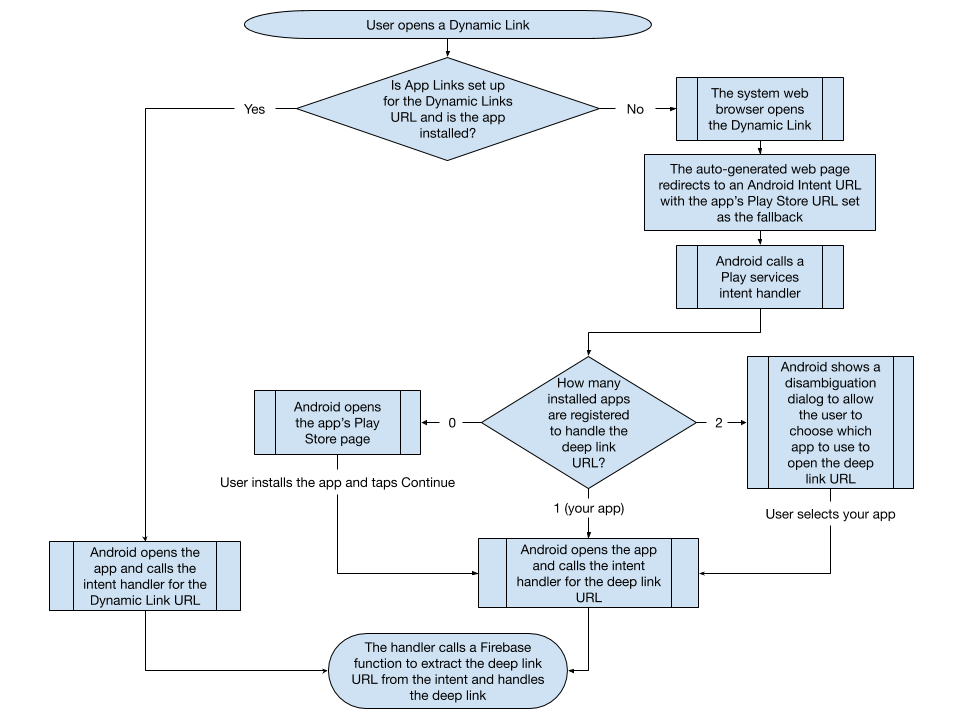
\includegraphics[width=0.83\textwidth]{images/diagramas/fdl-android-integration.png}
  \caption{Funcionamento dos dynamic links \citep{linking_firebase}}
  \label{fig:23}
\end{figure}




\newpage

\subsection{Qualidade de código}

\newpage






%  
\chapter{Analise e especificação}

Na proposta de sistema está contido a descrição do modelo de negócio, onde serão identificados os principais
 problemas do modelo atual e será indicada a necessidade de implementação do software. Nesta proposta 
 estará também identificado os objetivos de negócio, conseguindo identificar o principal impacto deste 
 software neste modelo de negócio. Nesta proposta estará também contida a engenharia de software com toda 
 a especificação do projeto em mãos.


 \section{Modelo de negócio}

Este projeto surgiu com a necessidade da Motorline melhorar a comunicação e a experiência das 
empresas clientes e técnicos. 
Atualmente sempre que um técnico possui uma questão este deverá contactar o suporte técnico o que pode 
levar a sobrecarga deste, ou então este deverá se juntar ao grupo do Facebook de técnicos e colocar 
neste esta questão. Sempre que é necessário um manual de produto ou sempre que o utilizador pretender ver 
o catalogo este deverá se deslocar ao site da Motorline e procurar o produto no catálogo não possuindo um
acesso rápido a estes.
Visto que este processo acaba por não ser prático para o utilizador, foi então 
decidido suprir este problema com o projeto Install \& Go. Tendo estas questões em mente surgiu então 
a ideia de implementar um fórum de resolução de problemas.


 \section{Objetivos de negócio}

Este software visa minimizar o problema acima descrito. Visto que acontece que muitas das 
questões dos técnicos são comuns, então surgiu a ideia de implementar um fórum onde o técnico poderá 
pesquisar por questões semelhantes à sua, encontrando solução sem necessidade de contactar o suporte 
técnico. O técnico poderá também expor a sua questão anexando imagens, facilitando o processo de 
resolução da sua questão. Para existir partilha de conhecimento o técnico poderá também responder 
a tópicos, pois caso encontre alguma questão que já tenha resolvido poderá ajudar outro técnico. O técnico 
também poderá alterar a visibilidade do seu tópico caso deseje que apenas técnicos visualizem a sua questão.

A empresa poderá realizar as mesmas ações que o técnico, mas esta poderá também criar contas para os seus 
técnicos e realizar a gestão destas sendo importante permitir apagar e impedir acesso à conta em caso de 
necessidade.


 \section{Estudo de Soluções existentes}
 Para ser possível entender todo o negócio onde o projeto se encaixa foi realizado um estudo
 que engloba outras soluções do mesmo ramo. Estas soluções investigadas foram indicações do supervisor de estágio, pois este já tinha realizado um estudo da situação do negócio préviamente. As soluções investigadas foram, \textit{FixAndGo}, \textit{My VDS} e \textit{Ultimate Cardin}. A solução \textit{FixAndGo} foi indicada devido à capacidade de calcular a possibilidade de instalar um motor com base em medidas indicadas pelo utilizador. Já a solução \textit{My VDS} foi mencionada devido ao facto de dispor de documentação sobre os seus produtos como manuais, vídeos e uma forma de comunicação com a equipa de suporte. Por fim, a solução \textit{Ultimate Cardin} foi utilizada como exemplo de \textit{design} a não seguir, devido a ser confuso, esta foi também utilizada como exemplo de organização de design do ecrã de detalhes de produto.

 \section{Domínio de aplicação do sistema}

Com o diagrama da Figura~\ref{fig:2} é possível visualizar todos os atores do \textit{software} e as suas ações, assim como os sistemas envolvidos na aplicação e as funções.
Destes é possível identificar que este \textit{software} contém três atores principais, o Utilizador que é um utilizador sem sessão iniciada, o Técnico, um utilizador com sessão iniciada, já a Empresa é uma empresa cliente da Motorline. Também é possível visualizar os diferentes sistemas integrados no projeto, como Servidor Motorline onde serão obtidas informações do catálogo de produtos, Servidor \textit{Install \& Go} onde estão todas as funções de suporte ao \textit{software}, o Servidor de Imagens onde serão guardadas todas as imagens da aplicação e por fim o Servidor de \textit{Email} que enviará \textit{email} com o código de validação de conta para os clientes assim que se registarem no \textit{software}.

\begin{figure}[htb]
  \centering
  
  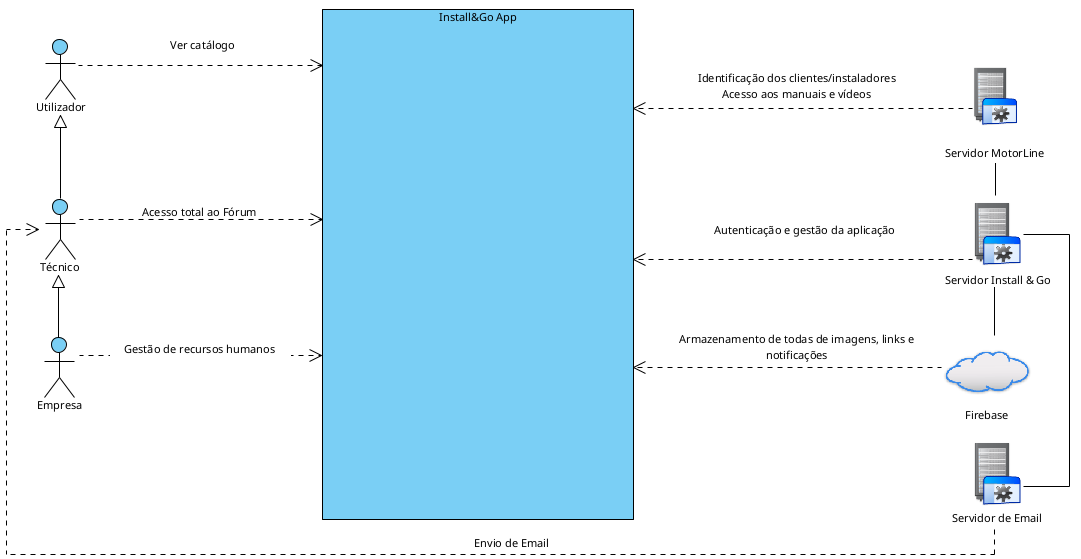
\includegraphics[width=\textwidth]{images/diagramas/diagrama_contexto.png}
  \caption{Diagrama de contexto da aplicação}
  \label{fig:2}
\end{figure}

 \newpage

 \section{Operações a realizar no sistema}
A primeira tarefa a realizar no desenvolvimento desta etapa do projeto foi o levantamento dos requisitos funcionais(Tabela~\ref{tab:1}) e não funcionais, tendo sido posteriormente validados com cliente. 

\definecolor{Mercury}{rgb}{0.905,0.901,0.901}
\begin{longtblr}
[
caption={Tabela de requisitos funcionais},
label={tab:1},
]
{
  width = \linewidth,
  colspec = {Q[75]Q[400]Q[160]Q[120]},
  row{1} = {Mercury},
  row{2} = {Mercury,c},
  row{10} = {Mercury,c},
  row{20} = {Mercury,c},
  row{26} = {Mercury,c},
  row{31} = {Mercury,c},
  row{35} = {Mercury,c},
  row{40} = {Mercury,c},
  row{45} = {Mercury,c},
  row{50} = {Mercury,c},
  cell{1}{1} = {c},
  cell{1}{3} = {c},
  cell{1}{4} = {c},
  cell{3}{1} = {c},
  cell{3}{3} = {c},
  cell{3}{4} = {c},
  cell{4}{1} = {c},
  cell{4}{3} = {c},
  cell{4}{4} = {c},
  cell{5}{1} = {c},
  cell{5}{3} = {c},
  cell{5}{4} = {c},
  cell{6}{1} = {c},
  cell{6}{3} = {c},
  cell{6}{4} = {c},
  cell{7}{1} = {c},
  cell{7}{3} = {c},
  cell{7}{4} = {c},
  cell{8}{1} = {c},
  cell{8}{3} = {c},
  cell{8}{4} = {c},
  cell{9}{1} = {c},
  cell{9}{3} = {c},
  cell{9}{4} = {c},
  cell{11}{1} = {c},
  cell{11}{3} = {c},
  cell{11}{4} = {c},
  cell{12}{1} = {c},
  cell{12}{3} = {c},
  cell{12}{4} = {c},
  cell{13}{1} = {c},
  cell{13}{3} = {c},
  cell{13}{4} = {c},
  cell{14}{1} = {c},
  cell{14}{3} = {c},
  cell{14}{4} = {c},
  cell{15}{1} = {c},
  cell{15}{3} = {c},
  cell{15}{4} = {c},
  cell{16}{1} = {c},
  cell{16}{3} = {c},
  cell{16}{4} = {c},
  cell{17}{1} = {c},
  cell{17}{3} = {c},
  cell{17}{4} = {c},
  cell{18}{1} = {c},
  cell{18}{3} = {c},
  cell{18}{4} = {c},
  cell{19}{1} = {c},
  cell{19}{3} = {c},
  cell{19}{4} = {c},
  cell{21}{1} = {c},
  cell{21}{3} = {c},
  cell{21}{4} = {c},
  cell{22}{1} = {c},
  cell{22}{3} = {c},
  cell{22}{4} = {c},
  cell{23}{1} = {c},
  cell{23}{3} = {c},
  cell{23}{4} = {c},
  cell{24}{1} = {c},
  cell{24}{3} = {c},
  cell{24}{4} = {c},
  cell{25}{1} = {c},
  cell{25}{3} = {c},
  cell{25}{4} = {c},
  cell{27}{1} = {c},
  cell{27}{3} = {c},
  cell{27}{4} = {c},
  cell{28}{1} = {c},
  cell{28}{3} = {c},
  cell{28}{4} = {c},
  cell{29}{1} = {c},
  cell{29}{3} = {c},
  cell{29}{4} = {c},
  cell{30}{1} = {c},
  cell{30}{3} = {c},
  cell{30}{4} = {c},
  cell{32}{1} = {c},
  cell{32}{3} = {c},
  cell{32}{4} = {c},
  cell{33}{1} = {c},
  cell{33}{3} = {c},
  cell{33}{4} = {c},
  cell{34}{1} = {c},
  cell{34}{3} = {c},
  cell{34}{4} = {c},
  cell{36}{1} = {c},
  cell{36}{3} = {c},
  cell{36}{4} = {c},
  cell{37}{1} = {c},
  cell{37}{3} = {c},
  cell{37}{4} = {c},
  cell{38}{1} = {c},
  cell{38}{3} = {c},
  cell{38}{4} = {c},
  cell{39}{1} = {c},
  cell{39}{3} = {c},
  cell{39}{4} = {c},
  cell{41}{1} = {c},
  cell{41}{3} = {c},
  cell{41}{4} = {c},
  cell{42}{1} = {c},
  cell{42}{3} = {c},
  cell{42}{4} = {c},
  cell{43}{1} = {c},
  cell{43}{3} = {c},
  cell{43}{4} = {c},
  cell{44}{1} = {c},
  cell{44}{3} = {c},
  cell{44}{4} = {c},
  cell{46}{1} = {c},
  cell{46}{3} = {c},
  cell{46}{4} = {c},
  cell{47}{1} = {c},
  cell{47}{3} = {c},
  cell{47}{4} = {c},
  cell{48}{1} = {c},
  cell{48}{3} = {c},
  cell{48}{4} = {c},
  cell{49}{1} = {c},
  cell{49}{3} = {c},
  cell{49}{4} = {c},
  cell{51}{1} = {c},
  cell{51}{3} = {c},
  cell{51}{4} = {c},
  cell{52}{1} = {c},
  cell{52}{3} = {c},
  cell{52}{4} = {c},
  cell{53}{1} = {c},
  cell{53}{3} = {c},
  cell{53}{4} = {c},
  cell{54}{1} = {c},
  cell{54}{3} = {c},
  cell{54}{4} = {c},
  hlines,
  vlines,
}
\#   & Descrição                                                                                                                                                           & Fonte          & Data      \\
     & Autenticação                                                                                                                                                        &                &           \\
RF01 & O Utilizador deverá conseguir visualizar o catálogo e ver as questões públicas do fórum, mas não deverá conseguir realizar operações sem realizar o login           & Helder Remelhe & 2/13/2023 \\
RF02 & A Empresa deverá conseguir realizar o registo na aplicação                                                                                                          & Helder Remelhe & 2/13/2023 \\
RF03 & O Técnico deverá conseguir realizar o login na aplicação                                                                                                            & Helder Remelhe & 2/13/2023 \\
RF04 & O login deverá ser realizado utilizando número de contribuinte e password                                                                                           & Helder Remelhe & 2/13/2023 \\
RF05 & Assim que o registo é realizado, a motorline deverá validar a conta sendo posteriormente enviado um email para a empresa ativar e utilizar a conta                  & Rafael Viana   & 2/13/2023 \\
RF06 & O Técnico deverá conseguir pedir reenvio de código de verificação de conta                                                                                          & Rafael Viana   & 2/27/2023 \\
RF07 & Os Técnicos deverão ser identificados como técnicos certificados ou técnicos oficiais                                                                               & Helder Remelhe & 2/27/2023 \\
     & Fórum                                                                                                                                                               &                &           \\
RF08 & O Técnico deverá conseguir aceder ao fórum e realizar operações                                                                                                     & Helder Remelhe & 2/13/2023 \\
RF09 & O Utilizador deverá conseguir visualizar os tópicos mais recentes                                                                                                      & Brainstorming  & 2/14/2023 \\
RF10 & O Utilizador deverá conseguir visualizar os tópicos em destaque                                                                                                        & Brainstorming  & 2/14/2023 \\
RF11 & O Utilizador deverá conseguir visualizar os tópicos por responder                                                                                                      & Brainstorming  & 2/14/2023 \\
RF12 & O Técnico deverá conseguir acessar aos tópicos privados do fórum                                                                                                    & Helder Remelhe & 2/13/2023 \\
RF13 & O Utilizador deverá conseguir pesquisar por tópicos referentes a um assunto desejado                                                                                   & Brainstorming  & 2/14/2023 \\
RF14 & O Utilizador deverá conseguir pesquisar por tópicos referentes a um produto desejado                                                                                   & Brainstorming  & 2/14/2023 \\
RF15 & O Utilizador deverá conseguir pesquisar por tópicos referentes a um produto por código QR                                                                              & Brainstorming  & 2/14/2023 \\
RF16 & O Técnico deverá conseguir visualizar os seus tópicos                                                                                                               & Brainstorming  & 2/14/2023 \\
     & Criar Tópico                                                                                                                                                        &                &           \\
RF17 & O Técnico deverá conseguir criar tópicos para expor a sua questão                                                                                                   & Helder Remelhe & 2/13/2023 \\
RF18 & O Técnico deverá conseguir colocar o seu tópico público ou privado para assim apenas outras empresas conseguirem ver                                                & Helder Remelhe & 2/13/2023 \\
RF19 & O Técnico deverá conseguir indicar tipo de tópico para agilizar a identificação do mesmo                                                                           & Helder Remelhe & 2/14/2023 \\
RF20 & O Técnico deverá conseguir indicar o produto referente ao tópico para agilizar a identificação da sua questão                                                      & Brainstorming  & 2/14/2023 \\
RF21 & O Técnico deverá conseguir anexar imagens ou vídeos ao tópico em questão para agilizar a comunicação e identificação do seu problema                               & Helder Remelhe & 2/13/2023 \\
     & Gestão de tópico                                                                                                                                                    &                &           \\
RF22 & O Técnico deverá conseguir indicar qual a melhor resposta ao seu tópico para assim facilitar a pesquisa por resposta a outras empresas que possuam o mesmo problema & Helder Remelhe & 2/14/2023 \\
RF23 & O Técnico deverá conseguir indicar que o tópico se encontra finalizado quando o seu problema se encontrar resolvido                                                 & Helder Remelhe & 2/13/2023 \\
RF24 & O Técnico deverá conseguir remover o seu tópico                                                                                                                     & Brainstorming  & 2/14/2023 \\
RF25 & O Técnico deverá conseguir alterar a visibilidade do seu tópico                                                                                                     & Helder Remelhe & 2/13/2023 \\
     & Tópicos                                                                                                                                                             &                &           \\*
RF26 & O Utilizador deverá conseguir ver todas as respostas ao tópico                                                                                                         & Helder Remelhe & 2/13/2023 \\
RF27 & O Técnico deverá conseguir gostar do tópico para dar destaque ao mesmo                                                                                              & Brainstorming  & 2/14/2023 \\
RF28 & O Técnico deverá conseguir remover uma resposta que colocou em um tópico                                                                                            & Brainstorming  & 2/14/2023 \\
     & Respostas a Tópicos                                                                                                                                                 &                &           \\
RF29 & O Técnico deverá conseguir comentar tópicos                                                                                                                         & Helder Remelhe & 2/13/2023 \\
RF30 & O Técnico deverá conseguir responder a comentários de tópicos                                                                                                       & Helder Remelhe & 2/13/2023 \\
RF31 & O Técnico deverá conseguir anexar imagens e videos à sua resposta                                                                                                   & Helder Remelhe & 2/13/2023 \\
RF32 & O Técnico deverá conseguir gostar de alguma resposta para dar destaque a esta resposta                                                                              & Helder Remelhe & 2/13/2023 \\
     & Perfil                                                                                                                                                              &                &           \\
RF33 & O Técnico deverá conseguir alterar o seu email                                                                                                                      & Helder Remelhe & 2/27/2023 \\
RF34 & O Técnico deverá conseguir alterar imagem de perfil                                                                                                                 & Brainstorming  & 2/27/2023 \\
RF35 & O Técnico deverá conseguir alterar nome                                                                                                                             & Brainstorming  & 2/27/2023 \\
RF36 & O Técnico deverá ser identificado como Técnico oficial ou certificado                                                                                                & Helder Remelhe & 2/28/2023 \\
     & Notificações                                                                                                                                                        &                &           \\
RF37 & O Técnico deverá conseguir receber notificações por email e/ou push                                                                                                 & Rafael Viana   & 2/27/2023 \\
RF38 & O Técnico deverá conseguir alterar o tipo de notificação ente relatório diário e notificação direta para ambos os tipos                                             & Rafael Viana   & 2/27/2023 \\
RF39 & O Técnico deverá conseguir ver as suas notificações                                                                                                                 & Helder Remelhe & 2/27/2023 \\
RF40 & O Técnico deverá conseguir apagar as suas notificações                                                                                                              & Helder Remelhe & 2/27/2023 \\
     & Gestão de recursos humanos                                                                                                                                          &                &           \\*
RF41 & A Empresa deverá conseguir criar contas para os seus técnicos                                                                                                       & Brainstorming  & 2/13/2023 \\*
RF42 & Assim que a conta de técnico for criada, este deverá receber um email para registar as restantes informações e ativar a conta                                       & Helder Remelhe & 2/27/2023 \\
RF43 & A Empresa deverá conseguir impedir acesso a uma conta de técnico                                                                                                    & Helder Remelhe & 2/27/2023 \\
RF44 & A Empresa deverá conseguir remover uma conta de técnico da empresa                                                                                                  & Helder Remelhe & 2/27/2023 
\end{longtblr}

 \section{Descrição dos intervenientes}
O projeto envolve um conjunto de intervenientes, sendo estes, o utilizador, a empresa e o técnico. Estes desempenham um papel fundamental e podem realizar diferentes ações.

O utilizador, sem sessão iniciada terá um fácil e rápido acesso ao catálogo de produtos, o que irá facilitar quando este desejar realizar a consulta do mesmo.

O técnico conseguirá realizar as mesmas ações que o utilizador, mas este ator conseguirá também ter acesso total ao fórum e se for técnico oficial tem também acesso a questões privadas. O fórum permite expor questões, com auxílio de imagens, a ligação da questão a uma categoria de questões e um produto em específico para facilitar a resolução da questão. As questões poderão ser públicas para qualquer um, ou então estas podem ser privadas para apenas técnicos oficiais conseguirem ver. Assim que o técnico estiver satisfeito com a questão poderá indicar a melhor resposta obtida ao problema sendo esta destacada e a publicação finalizada.

O técnico pode realizar pesquisas por questões, onde evita um telefonema ou o preenchimento de um formulário para contactar um técnico oficial. Com estas pesquisas poderá responder a outras questões, pode pesquisar por questões em categoria. As respostas podem conter imagens anexadas e podem responder a outras respostas para manter uma comunicação continua. O técnico poderá destacar publicações e respostas de publicações com um \textit{like}.

A empresa pode realizar a gestão de contas de técnicos, onde cria, impede acesso e 
eliminar em caso de necessidade.


 \section{Partes Interessadas}

Este projeto foi proposto pelo supervisor de estágio, sendo então este com a empresa Motorline representada 
por, Rafael Viana e André Viana, as partes interessadas.

 \newpage
\section{Condições Específicas}

Os requisitos não funcionais são caraterísticas do software que não interferem diretamente com o 
funcionamento normal do software, estes podem referir-se a caraterísticas como segurança e culta. 
Na Tabela~\ref{tab:2} é possível visualizar os requisitos não funcionais levantados.

\definecolor{Alto}{rgb}{0.85,0.85,0.85}
\begin{table}[htb]
\centering
\caption{Tabela de requisitos não funcionais}
\label{tab:2}
\begin{tblr}{
  width = \linewidth,
  colspec = {Q[77]Q[215]Q[638]},
  row{1} = {Alto},
  hlines,
  vlines,
  vline{3} = {-}{black},
}
\#    & Tipo            & Descrição                                                                        \\
RNF01 & Cultural        & O software tem de suportar vários idiomas (prioritariamente, português e inglês) \\
RNF02 & Configuração    & A falha dos servidores, implica a inutilidade total da aplicação                 \\
RNF03 & Conexão         & Necessário o uso de dados móveis ou WIFI                                         \\
RNF04 & Segurança       & O software tem de ser seguro para proteger os dados do consumidor          \\
RNF05 & Desenvolvimento & A aplicação deverá ser desenvolvida utilizando a tecnologia flutter              
\end{tblr}
\end{table}

 
 \newpage

 \section{Esquematização do conteúdo das páginas}

Para ser possibilitar a perceção dos dados necessários para alimentar o \textit{software}, o que apresentar em cada página e também como navegar entre os ecrãs da aplicação foi então desenhado um esquema 
(Figura~\ref{fig:3}).

\begin{figure}[htb]
  \centering
  
  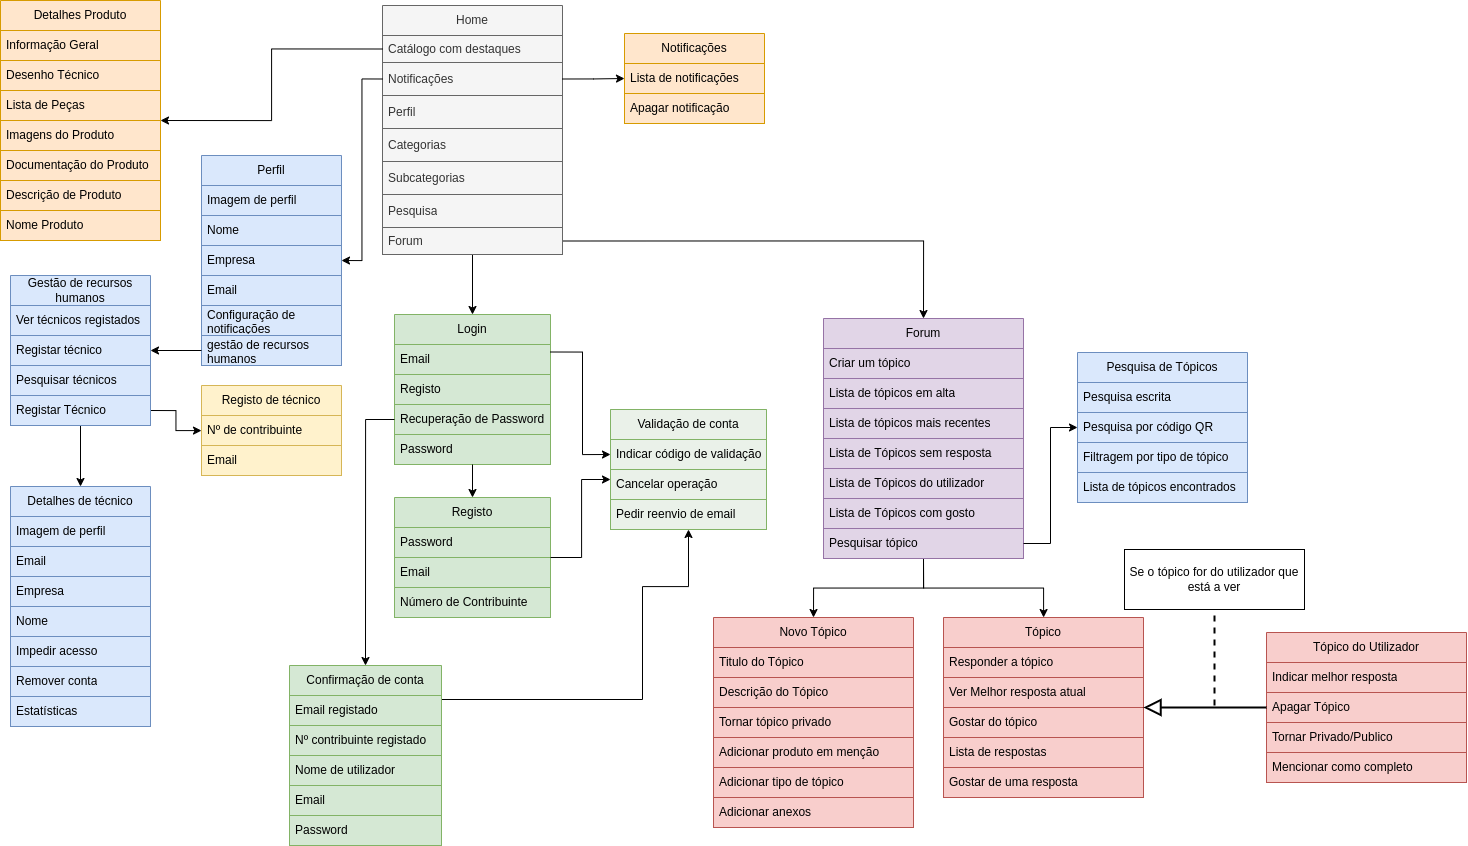
\includegraphics[width=\textwidth]{images/Arquiteturas/diagrama_superficial_de_aplicacao.png}
  \caption{Esquema de organização de páginas do \textit{software}}
  \label{fig:3}
\end{figure}

\newpage

\subsection{Autenticação e página Inicial}

Através deste esquema é possível perceber que do ecrã principal, o utilizador tem acesso ao 
catálogo de produtos e ao fórum, neste pode também realizar o \textit{login} e o \textit{logout} que redirecionam para os respetivos ecrãs.

No ecrã de \textit{login} é necessário o utilizador indicar o número de contribuinte e a \textit{\textit{password}}, neste ele pode também pedir recuperação de \textit{\textit{password}} e/ou redirecionar para o registo onde necessitará de número de contribuinte, \textit{\textit{password}} e \textit{email} para o realizar.

Em caso de o utilizador não possuir a conta ativa, este será encaminhado para o ecrã de validação conta em que deverá indicar o código de validação, cancelar a operação e pedir o reenvio do código de validação.

Em caso de se tratar de um técnico que necessita de confirmar a sua conta, este conseguirá ver as informações registadas, introduzir o seu nome, alterar o seu \textit{email} e \textit{password}.

\begin{figure}[htb]
  \centering
  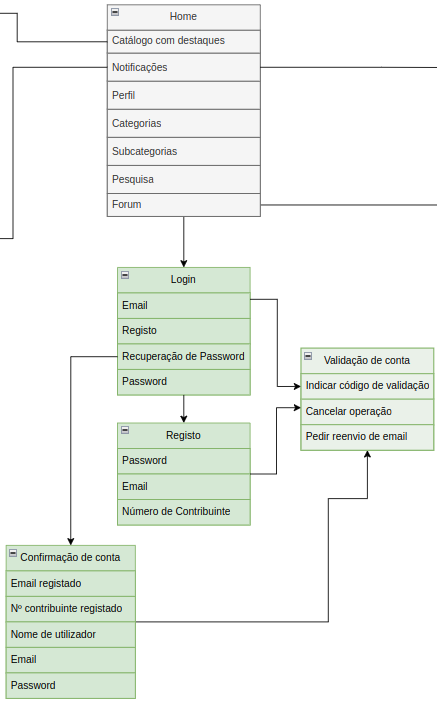
\includegraphics[height=0.9\textwidth]{images/Arquiteturas/superficial_de_app/home_auth.png}
  \caption{Esquema de organização das páginas de autenticação e página inicial}
  \label{fig:4}
\end{figure}

\newpage

\subsection{Fórum}

Através do ecrã inicial o utilizador pode direcionar-se para o ecrã do fórum. Neste ecrã, poderá pesquisar por tópicos, ou então aceder a tópicos em alta, mais recentes ou sem resposta.
O técnico consegue também criar e ver as suos tópicos.

\begin{figure}[htb]
  \centering
  
  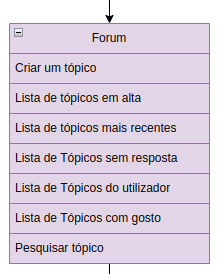
\includegraphics[height=0.4\textwidth]{images/Arquiteturas/superficial_de_app/forum.png}
  \caption{Esquema de organização da página de fórum}
  \label{fig:5}
\end{figure}

\subsection{Criar nova tópico}

Quando o técnico decide criar uma tópico, este tem de indicar o título e a descrição, de seguida poderá indicar se é privado ou não, o tipo de tópico, o produto referente e adicionar anexos.

\begin{figure}[htb]
  \centering
  
  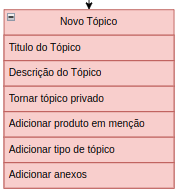
\includegraphics[height=0.3\textwidth]{images/Arquiteturas/superficial_de_app/criar_topico.png}
  \caption{Esquema de organização da página de criação de tópicos}
  \label{fig:6}
\end{figure}

\newpage

\subsection{Detalhes de tópicos}

O técnico pode também ver os detalhes da tópico, responder, 
gostar e gostar de uma resposta.
Caso esta seja do mesmo, este pode indicar a melhor resposta, apagar a tópico, tornar pública ou privada e indicar como completa.

\begin{figure}[htb]
  \centering
  
  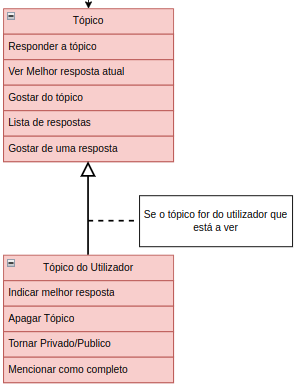
\includegraphics[height=0.55\textwidth]{images/Arquiteturas/superficial_de_app/detalhes_topico.png}
  \caption{Esquema de organização da página de detalhes de tópico}
  \label{fig:7}
\end{figure}

\subsection{Pesquisa de tópicos}

A página de pesquisa permite ao técnico procurar por tópicos específicos tanto por nome como por produto. Para além da pesquisa o utilizador pode também realizar a filtragem dos 
tópicos por tipo e categoria.
\begin{figure}[htb]
  \centering
  
  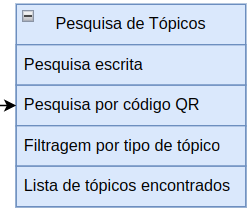
\includegraphics[height=0.3\textwidth]{images/Arquiteturas/superficial_de_app/pesquisa_forum.png}
  \caption{Esquema de organização da página de pesquisa de tópicos}
  \label{fig:8}
\end{figure}

\subsection{Notificações}

A página de notificações permite ao técnico visualizar as suas notificações, assim como também apagar.
\begin{figure}[htb]
  \centering
  
  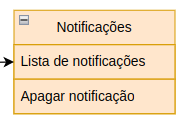
\includegraphics[height=0.2\textwidth]{images/Arquiteturas/superficial_de_app/notificacoes.png}
  \caption{Esquema de organização da página de notificações}
  \label{fig:9}
\end{figure}

\subsection{Perfil}

A página de perfil de técnico permite visualizar as suas informações, assim como alterar 
o seu \textit{email} e configurar as notificações. Caso se trate de uma empresa a visualizar o seu perfil, esta poderá ter acesso à gestão de recursos humanos, para gerir os seus técnicos.
\begin{figure}[htb]
  \centering
  
  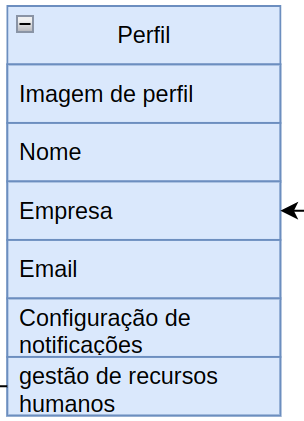
\includegraphics[height=0.35\textwidth]{images/Arquiteturas/superficial_de_app/perfil.png}
  \caption{Esquema de organização da página de perfil}
  \label{fig:10}
\end{figure}

\newpage

\subsection{Gestão de recursos humanos}

A página de gestão de recursos humanos permite à empresa gerir todos os seus técnicos registados e criar contas. Assim que a empresa seleciona um técnico, esta vê o seu perfil, 
com estatísticas.
\begin{figure}[htb]
  \centering
  
  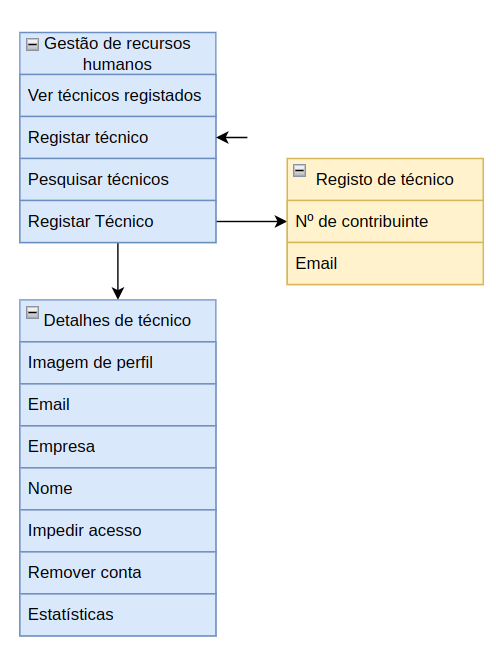
\includegraphics[height=0.7\textwidth]{images/Arquiteturas/superficial_de_app/gestao_recursos_humanos.png}
  \caption{Esquema de organização da página de gestão de recursos humanos}
  \label{fig:11}
\end{figure}

 \newpage

 \section{Histórias de Utilizador}
Antes de desenvolver os casos de uso foram criadas histórias de utilizador para ser possível descrever os objetivos ao realizar uma ação.

% \usepackage{color}
% \usepackage{tabularray}
\definecolor{Concrete}{rgb}{0.952,0.952,0.952}
\begin{longtblr}
[
caption={Tabela de histórias de utilizador},
label={tab:3},
]{
     width = \linewidth,
     colspec = {Q[75]Q[110]Q[700]},
     row{1} = {Concrete},
  row{2} = {Concrete},
  row{8} = {Concrete},
  row{19} = {Concrete},
  row{25} = {Concrete},
  row{30} = {Concrete},
  row{34} = {Concrete},
  row{39} = {Concrete},
  row{43} = {Concrete},
  row{47} = {Concrete},
  column{2} = {c},
  cell{1}{1} = {c},
  cell{2}{2} = {c=2}{0.891\linewidth},
  cell{3}{1} = {c},
  cell{4}{1} = {c},
  cell{5}{1} = {c},
  cell{8}{2} = {c=2}{0.891\linewidth},
  cell{9}{1} = {c},
  cell{10}{1} = {c},
  cell{11}{1} = {c},
  cell{12}{1} = {c},
  cell{13}{1} = {c},
  cell{14}{1} = {c},
  cell{15}{1} = {c},
  cell{16}{1} = {c},
  cell{17}{1} = {c},
  cell{18}{1} = {c},
  cell{19}{2} = {c=2}{0.891\linewidth},
  cell{20}{1} = {c},
  cell{21}{1} = {c},
  cell{22}{1} = {c},
  cell{23}{1} = {c},
  cell{24}{1} = {c},
  cell{25}{2} = {c=2}{0.891\linewidth},
  cell{26}{1} = {c},
  cell{27}{1} = {c},
  cell{28}{1} = {c},
  cell{29}{1} = {c},
  cell{30}{2} = {c=2}{0.891\linewidth},
  cell{31}{1} = {c},
  cell{32}{1} = {c},
  cell{33}{1} = {c},
  cell{34}{2} = {c=2}{0.891\linewidth},
  cell{35}{1} = {c},
  cell{36}{1} = {c},
  cell{37}{1} = {c},
  cell{38}{1} = {c},
  cell{39}{2} = {c=2}{0.891\linewidth},
  cell{40}{1} = {c},
  cell{41}{1} = {c},
  cell{42}{1} = {c},
  cell{43}{2} = {c=2}{0.891\linewidth},
  cell{44}{1} = {c},
  cell{45}{1} = {c},
  cell{46}{1} = {c},
  cell{47}{2} = {c=2}{0.891\linewidth},
  cell{48}{1} = {c},
  cell{49}{1} = {c},
  cell{50}{1} = {c},
  hlines,
  vlines,
}
\#   & Ator                       & Descrição                                                                                                                                                                              \\
     & Autenticação               &                                                                                                                                                                                        \\
US01 & Utilizador                 & Eu como Utilizador, quero conseguir utilizar a aplicação sem realizar o login                                                                                                          \\
US02 & Empresa                    & Eu como Empresa, quero conseguir realizar o registo na aplicação                                                                                                                       \\
US03 & Técnico                    & Eu como Técnico, quero conseguir realizar o login na aplicação utilizando o número de contribuinte e \textit{password}                                                                          \\
US04 & Técnico                    & Eu como Técnico, quero conseguir pedir reenvio de código de ativação de conta caso eu não receba o código                                                                              \\
US05 & Técnico                    & Eu como Técnico, quero conseguir ser identificado como tal na aplicação                                                                                                                \\
     & Fórum                      &                                                                                                                                                                                        \\*
US06 & Técnico                    & Eu como Técnico, quero conseguir acessar ao fórum                                                                                                                                      \\*
US07 & Técnico                    & Eu como Técnico, quero conseguir visualizar os tópicos mais recentes, de forma a conseguir ver os mais falados no dia atual                                                            \\
US08 & Técnico                    & Eu como Técnico, quero conseguir visualizar os tópicos em destaque, de forma a ver quais são mais falados                                                                      \\
US09 & Técnico                    & Eu como Técnico, quero conseguir ver os meus tópicos de forma a conseguir aceder a estes facilmente                                                                                    \\
US10 & Técnico                    & Eu como Técnico, quero conseguir visualizar os tópicos por responder, de forma a conseguir ajudar alguém com maior facilidade                                                          \\
US11 & Técnico                    & Eu como Técnico, quero conseguir visualizar os tópicos privados                                                                                                                        \\
US12 & Técnico                    & Eu como Técnico, quero conseguir realizar filtragem de tópicos por tipo                                                                                \\
US13 & Técnico                    & Eu como Técnico, quero conseguir pesquisar por um tópico relativo a um assunto de forma a obter a solução                                                                              \\
US14 & Técnico                    & Eu como Técnico, quero conseguir pesquisar por um tópico relativo a um produto de forma a encontrar questões comuns a este                                                             \\
US15 & Técnico                    & Eu como Técnico, quero conseguir pesquisar por código QR de um produto de forma a encontrar tópicos referentes ao mesmo mais facilmente                                                 \\
     & Criar Tópico               &                                                                                                                                                                                        \\*
US16 & Técnico                    & Eu como Técnico, quero conseguir criar tópicos de forma a conseguir expor questões                                                                                                     \\*
US17 & Técnico                    & Eu como Técnico, quero conseguir indicar se o meu tópico é publico ou privado, de forma a conseguir respostas de qualquer cliente, ou apenas de técnicos                               \\*
US18 & Técnico                    & Eu como Técnico, quero conseguir indicar o tipo de tópico em que o este se enquadra de forma a facilitar a sua identificação                                                          \\*
US19 & Técnico                    & Eu como Técnico, quero conseguir indicar o produto referente ao tópico para facilitar a identificação do mesmo                                                                         \\*
US20 & Técnico                    & Eu como Técnico, quero conseguir anexar imagens ao tópico de forma a facilitar a comunicação e identificação do problema                                                               \\*
     & Gestão de Tópico           &                                                                                                                                                                                        \\*
US21 & Técnico                    & Eu como Técnico quero conseguir indicar qual a melhor resposta ao meu tópico de forma a facilitar o encontro da solução do problema a outros clientes ou técnicos com o mesmo problema \\*
US22 & Técnico                    & Eu como Técnico quero conseguir indicar que o tópico se encontra finalizado quando o problema está resolvido                                                                           \\
US23 & Técnico                    & Eu como Técnico quero conseguir remover o meu tópico                                                                                                                                   \\
US24 & Técnico                    & Eu como Técnico quero conseguir alterar a visibilidade do meu tópico                                                                                                                   \\
     & Tópicos                    &                                                                                                                                                                                        \\
US25 & Técnico                    & Eu como Técnico, quero conseguir ver todas as respostas a um tópico                                                                                                                    \\
US26 & Técnico                    & Eu como Técnico, quero conseguir gostar de um tópico caso o ache relevante                                                                                                             \\
US27 & Técnico                    & Eu como Técnico, quero conseguir apagar uma resposta minha                                                                                                                             \\
     & Respostas a Tópicos        &                                                                                                                                                                                        \\
US28 & Técnico                    & Eu como Técnico, quero conseguir comentar um tópico de forma a dar a minha resposta                                                                                                    \\
US29 & Técnico                    & Eu como Técnico, quero conseguir responder a um comentário de forma a comunicar                                                                                                        \\
US30 & Técnico                    & Eu como Técnico, quero conseguir anexar imagens ao meu comentário                                                                                                                      \\
US31 & Técnico                    & Eu como Técnico, quero conseguir gostar de um comentário caso ache este relevante                                                                                                      \\
     & Perfil                     &                                                                                                                                                                                        \\*
US32 & Técnico                    & Eu como Técnico quero conseguir alterar o meu \textit{email}                                                                                                                                    \\*
US33 & Técnico                    & Eu como Técnico quero conseguir alterar a minha imagem de perfil                                                                                                                       \\*
US34 & Técnico                    & Eu como Técnico quero conseguir alterar o meu nome                                                                                                                                     \\*
     & Notificações               &                                                                                                                                                                                        \\
US35 & Técnico                    & Eu como Técnico quero conseguir receber notificações por \textit{email} e/ou push de forma a manter-me atualizado das minhas questões                                                           \\
US36 & Técnico                    & Eu como Técnico quero conseguir alterar o tipo de notificação que recebo entre relatório diário e tempo real                                                                           \\
US37 & Técnico                    & Eu como Técnico quero conseguir apagar as minhas notificações de forma a evitar aglomeração                                                                                            \\
     & Gestão de recursos humanos &                                                                                                                                                                                        \\*
US38 & Empresa                    & Eu como Empresa quero conseguir criar conta para os meus técnicos utilizarem o fórum                                                                                                   \\
US39 & Empresa                    & Eu como Empresa quero conseguir impedir acesso a uma conta de técnico                                                                                                                  \\
US40 & Empresa                    & Eu como Empresa quero conseguir remover uma conta de técnico em caso de este já não pertencer à empresa                                                                                
\end{longtblr}

  \newpage

 \section{Casos de uso}
Para transformar as histórias de utilizador em ações e especificar todas as reações do sistema com o qual o ator interage foram desenvolvidos casos de uso.

% \usepackage{color}
% \usepackage{tabularray}
\definecolor{Concrete}{rgb}{0.952,0.952,0.952}
\definecolor{Gallery}{rgb}{0.937,0.937,0.937}
\begin{longtblr}
[
caption={Tabela de casos de uso},
label={tab:4},
]
{
  width = \linewidth,
  colspec = {Q[130]Q[81]Q[120]Q[242]Q[375]},
  row{1} = {Concrete},
  row{2} = {Concrete,c},
  row{4} = {Concrete,c},
  row{8} = {Concrete,c},
  row{10} = {Concrete,c},
  row{18} = {Concrete,c},
  row{23} = {Concrete,c},
  row{26} = {Concrete,c},
  row{28} = {Concrete,c},
  row{31} = {Concrete,c},
  column{2} = {c},
  column{3} = {c},
  cell{1}{1} = {c},
  cell{2}{1} = {c=5}{0.936\linewidth},
  cell{4}{1} = {c=5}{0.936\linewidth},
  cell{8}{1} = {c=5}{0.936\linewidth},
  cell{10}{1} = {c=5}{0.936\linewidth},
  cell{18}{1} = {c=5}{0.936\linewidth},
  cell{23}{1} = {c=5}{0.936\linewidth},
  cell{26}{1} = {c=5}{0.936\linewidth},
  cell{28}{1} = {c=5}{0.936\linewidth},
  cell{31}{1} = {c=5}{0.936\linewidth},
  hlines,
  vlines,
}
\#                         & User Story         & Ator       & Nome                                & Descrição                                                   \\
Criar tópico               &                    &            &                                     &                                                             \\
UC 1.0                     & US15               & Técnico    & Criar novo tópico                   & Criação de um novo tópico no fórum                          \\
Pesquisa de tópicos        &                    &            &                                     &                                                             \\
UC 1.1                     & US11               & Técnico    & Pesquisar tópicos específicos       & Pesquisar por tópicos no fórum                              \\
UC 1.1.1                   & US12 e US13        & Técnico    & Pesquisa escrita                    & Pesquisar tópicos por assunto                               \\
UC 1.1.2                   & US14               & Técnico    & Pesquisa por código QR              & Pesquisar tópicos referentes a um produto                   \\
Listagens de tópicos       &                    &            &                                     &                                                             \\
UC 1.2                     & US05               & Técnico    & Ver tópicos                         & Ver listagens de tópicos do fórum                           \\
Detalhes de tópico         &                    &            &                                     &                                                             \\
UC 1.3                     & US08               & Técnico    & Selecionar tópico                   & Ver detalhes de um tópico selecionado                       \\
UC 1.3.1                   & US21               & Técnico    & Finalizar tópico                    & Finalizar um tópico para indicar que está respondido        \\
UC 1.3.2                   & US20               & Técnico    & Selecionar melhor resposta          & Selecionar a melhor resposta do tópico                      \\
UC 1.3.3                   & US22               & Técnico    & Eliminar tópico                     & Eliminar um tópico do fórum                                 \\
UC 1.3.4                   & US23               & Técnico    & Alterar visibilidade do tópico      & Alterar a visibilidade de um tópico entre publico e privado \\
UC 1.3.5                   & US28               & Técnico    & Comentar o tópico                   & Comentar um tópico                                          \\
UC 1.3.6                   & US25               & Técnico    & Gostar de tópico                    & Gostar de um tópico                                         \\
Comentários                &                    &            &                                     &                                                             \\
UC 1.3.7                   & US24               & Técnico    & Ver comentários                     & Ver comentários do tópico                                   \\
UC 1.3.7.1                 & US27               & Técnico    & Apagar comentário                   & Apagar comentário de um tópico                              \\
UC 1.3.7.2                 & US29               & Técnico    & Responder a comentário              & Responder a um comentário de um tópico                      \\
UC 1.3.7.3                 & US31               & Técnico    & Gostar de comentário                & Gostar de um comentário                                     \\
Ativação de conta          &                    &            &                                     &                                                             \\
UC 1.4                     & -                  & Técnico    & Ativação de conta                   & Ativar conta de cliente                                     \\
UC 1.4.1                   & US04               & Técnico    & Pedir reenvio de código de ativação & Pedir reenvio de email de código de ativação                \\
Perfil                     &                    &            &                                     &                                                             \\
UC 1.5                     & US31 - US32 - US33 & Técnico    & Ver Perfil                          & Ver perfil de utilizador                                    \\
Notificações               &                    &            &                                     &                                                             \\
UC1.6                      & US34 e US36        & Técnico    & Ver notificações                    & Ver todas as notificações                                   \\
UC1.7                      & US34 e US35        & Técnico    & Configuração de notificações        & Configurar o modo e tipo de notificações a receber          \\
Gestão de recursos humanos &                    &            &                                     &                                                             \\
UC1.8                      & US37               & Empresa    & Registar Técnico                    & Registar conta de técnico da empresa                        \\
UC1.9                      & US38               & Empresa    & Impedir acesso a técnico            & Registar conta de técnico da empresa                        \\
UC1.10                     & US39               & Empresa    & Remover conta de técnico            & Registar conta de técnico da empresa                        
\end{longtblr}
\newpage

\subsection{Especificação de casos de uso}

Para demonstrar todas as interações entre os atores e o sistema, assim como todas as ações e fluxos possíveis, foram realizadas especificações de casos de uso.

\subsubsection{Especificação de caso de uso de listagem de tópicos}

Através da listagem de tópicos é possível visualizar todas as listagens que o utilizador poderá visualizar, sendo que, o técnico oficial consegue para além destas listagens, ver os seus tópicos e os tópicos privados.

%\definecolor{Concrete}{rgb}{0.952,0.952,0.952}
\begin{longtblr}
[
caption={Tabela de especificação de caso de uso de listagem de tópicos do utilizador},
label={tab:8},
]
{
  width = \linewidth,
  colspec = {Q[225]Q[331]Q[383]},
  row{6} = {Concrete},
  cell{1}{1} = {Concrete},
  cell{1}{2} = {c=2}{0.714\linewidth},
  cell{2}{1} = {Concrete},
  cell{2}{2} = {c=2}{0.714\linewidth},
  cell{3}{1} = {Concrete},
  cell{3}{2} = {c=2}{0.714\linewidth},
  cell{4}{1} = {Concrete},
  cell{4}{2} = {c=2}{0.714\linewidth,c},
  cell{5}{1} = {Concrete},
  cell{5}{2} = {c=2}{0.714\linewidth,c},
  cell{6}{2} = {c},
  cell{6}{3} = {c},
  cell{7}{1} = {r=2}{Concrete},
  cell{9}{1} = {r=2}{Concrete},
  cell{11}{1} = {r=2}{Concrete},
  vlines,
  hline{1-7,9,11,13} = {-}{},
  hline{8,10,12} = {2-3}{},
}
Caso de Uso           & Ver listagem de tópicos                                               &                                  \\
Descrição             & Ver a listagem de tópicos existentes no fórum por diversas categorias &                                  \\
Ator                  & Utilizador                                                            &                                  \\
Pré-condição          & -                                                                     &                                  \\
Pós-condição          & -                                                                     &                                  \\
                      & Ator                                                                  & Sistema                          \\
Fluxo Principal       & 1-Ver tópicos populares                                               &                                  \\
                      &                                                                       & 2-Lista de tópicos populares     \\
Fluxo Alternativo(A1) & 1-Ver tópicos mais recentes                                           &                                  \\
                      &                                                                       & 2-Lista de tópicos mais recentes \\
Fluxo Alternativo(A2) & 1-Ver tópicos por responder                                           &                                  \\
                      &                                                                       & 2-Lista de tópicos por responder 
\end{longtblr}

\definecolor{Concrete}{rgb}{0.952,0.952,0.952}
\begin{longtblr}
[
caption={Tabela de especificação de caso de uso de listagem de tópicos do técnico},
label={tab:5},
]
{
  width = \linewidth,
  colspec = {Q[225]Q[331]Q[383]},
  row{6} = {Concrete},
  cell{1}{1} = {Concrete},
  cell{1}{2} = {c=2}{0.714\linewidth},
  cell{2}{1} = {Concrete},
  cell{2}{2} = {c=2}{0.714\linewidth},
  cell{3}{1} = {Concrete},
  cell{3}{2} = {c=2}{0.714\linewidth},
  cell{4}{1} = {Concrete},
  cell{4}{2} = {c=2}{0.714\linewidth,c},
  cell{5}{1} = {Concrete},
  cell{5}{2} = {c=2}{0.714\linewidth,c},
  cell{6}{2} = {c},
  cell{6}{3} = {c},
  cell{7}{1} = {r=2}{Concrete},
  cell{9}{1} = {r=2}{Concrete},
  cell{11}{1} = {r=2}{Concrete},
  cell{13}{1} = {r=2}{Concrete},
  vlines,
  hline{1-7,9,11,13,15} = {-}{},
  hline{8,10,12,14} = {2-3}{},
}
Caso de Uso           & Ver listagem de tópicos                                               &                                  \\
Descrição             & Ver a listagem de tópicos existentes no fórum por diversas categorias &                                  \\
Ator                  & Técnico                                                            &                                  \\
Pré-condição          & -                                                                     &                                  \\
Pós-condição          & -                                                                     &                                  \\
                      & Ator                                                                  & Sistema                          \\
Fluxo Principal       & 1-Ver tópicos populares                                               &                                  \\
                      &                                                                       & 2-Lista de tópicos populares     \\
Fluxo Alternativo(A1) & 1-Ver tópicos mais recentes                                           &                                  \\
                      &                                                                       & 2-Lista de tópicos mais recentes \\
Fluxo Alternativo(A2) & 1-Ver meus tópicos                                                    &                                  \\
                      &                                                                       & 2-Lista de tópicos do técnico    \\
Fluxo Alternativo(A3) & 1-Ver tópicos por responder                                           &                                  \\
                      &                                                                       & 2-Lista de tópicos por responder 
\end{longtblr}

\newpage

\subsubsection{Especificação de caso de uso de criar novo tópico}

Aquando a criação de um tópico, um técnico poderá realizar diversas ações sendo que obrigatoriamente terá de indicar o título, descrição e tipo de tópico, para além desta informação o técnico poderá anexar imagens, referenciar um produto e indicar a visibilidade.

\definecolor{Concrete}{rgb}{0.952,0.952,0.952}
\begin{longtblr}
[
caption={Tabela de especificação de caso de uso login},
label={tab:6},
]{
 width = \linewidth,
 colspec = {Q[212]Q[360]Q[369]},
 row{6} = {Concrete},
 cell{1}{1} = {Concrete},
 cell{1}{2} = {c=2}{0.725\linewidth},
 cell{2}{1} = {Concrete},
 cell{2}{2} = {c=2}{0.725\linewidth},
 cell{3}{1} = {Concrete},
 cell{3}{2} = {c=2}{0.725\linewidth},
 cell{4}{1} = {Concrete},
 cell{4}{2} = {c=2}{0.725\linewidth},
 cell{5}{1} = {Concrete},
 cell{5}{2} = {c=2}{0.725\linewidth,c},
 cell{6}{2} = {c},
 cell{6}{3} = {c},
 cell{7}{1} = {r=10}{Concrete,c},
 cell{17}{1} = {Concrete},
 cell{18}{1} = {r=6}{Concrete},
 vlines,
 hline{1-7,17-18,24} = {-}{},
 hline{8-16,19-23} = {2-3}{},
}
Caso de Uso      & Criar novo tópico           &                    \\
Descrição       & Criação de um novo tópico no fórum   &                    \\
Ator         & Técnico                &                    \\
Pré-condição     & Clicar em adicionar novo tópico    &                    \\
Pós-condição     & -                   &                    \\
           & Ator                  & Sistema                \\
Fluxo Principal    & 1-Indicar o título do tópico      &                    \\
           & 2-Indicar a descrição do tópico    &                    \\
           & 3-Indicar se o tópico é privado    &                    \\
           & 4-Indicar o tipo do tópico       &                    \\
           & 5-Indicar o produto referido no tópico &                    \\
           & 6-Adicionar imagens de anexo      &                    \\
           & 7-Confirmar a criação do tópico    &                    \\
           &                    & 8-Verificar se titulo está inserido  \\
           &                    & 9-Verificar se descrição está inserida \\
           &                    & 10-Inserir novo tópico no fórum    \\
Fluxo Alternativo(A1) & 1-Cancelar a criação do tópico     &                    \\
Fluxo Alternativo(A2) & 1-Indicar o título do tópico      &                    \\*
           & 2-Indicar se o tópico é privado    &                    \\*
           & 3-Confirmar a criação do tópico    &                    \\*
           &                    & 4-Verificar se titulo está inserido  \\*
           &                    & 5-Verificar se descrição está inserida \\*
           &                    & 6-Erro descrição em falta     
\end{longtblr}

\newpage

\subsubsection{Especificação de caso de uso de pesquisar tópicos por escrito}

Assim que um técnico deseje pesquisar por um assunto específico de tópico este poderá realizar uma pesquisa escrita onde conseguirá realizar filtragem por tipo e categoria de tópico.

% \usepackage{color}
% \usepackage{tabularray}
\definecolor{Concrete}{rgb}{0.952,0.952,0.952}
\begin{longtblr}
[
caption={Tabela de especificação de caso de uso de pesquisa por escrito},
label={tab:6},
]{
  width = \linewidth,
  colspec = {Q[190]Q[217]Q[533]},
  row{6} = {Concrete},
  cell{1}{1} = {Concrete},
  cell{1}{2} = {c=2}{0.702\linewidth},
  cell{2}{1} = {Concrete},
  cell{2}{2} = {c=2}{0.702\linewidth},
  cell{3}{1} = {Concrete},
  cell{3}{2} = {c=2}{0.702\linewidth},
  cell{4}{1} = {Concrete},
  cell{4}{2} = {c=2}{0.702\linewidth},
  cell{5}{1} = {Concrete},
  cell{5}{2} = {c=2}{0.702\linewidth,c},
  cell{6}{2} = {c},
  cell{6}{3} = {c},
  cell{7}{1} = {r=4}{Concrete},
  cell{11}{1} = {r=2}{Concrete},
  vlines,
  hline{1-7,11,13} = {-}{},
  hline{8-10,12} = {2-3}{},
}
Caso de Uso           & Pesquisa por escrita           &                                            \\
Descrição             & Pesquisar por tópicos no fórum &                                            \\
Ator                  & Utilizador                     &                                            \\
Pré-condição          & Selecionar pesquisa de fórum   &                                            \\
Pós-condição          & -                              &                                            \\
                      & Ator                           & Sistema                                    \\
Fluxo Principal       & 1-Pesquisar assunto            &                                            \\
                      &                                & 2-Lista de tópicos do assunto              \\
                      & 3-Filtrar por tipo             &                                            \\
                      &                                & 3-Filtragem de tópicos do assunto por tipo \\
Fluxo Alternativo(A1) & 1-Pesquisar assunto            &                                            \\
                      &                                & 2-Lista de tópicos do assunto              
\end{longtblr}


\subsubsection{Especificação de caso de uso de ver finalizar tópico}

Quando um técnico encontra-se satisfeito com a solução do problema este poderá indicar que o tópico está finalizado, o que é sinalizado para outros técnicos.

% \usepackage{color}
% \usepackage{tabularray}
\definecolor{Concrete}{rgb}{0.952,0.952,0.952}
\begin{table}[htb]
\centering
\label{tab:8}
\caption{Tabela de especificação de caso de uso de finalizar tópico}
\begin{tblr}{
  width = \linewidth,
  colspec = {Q[254]Q[319]Q[365]},
  row{6} = {Concrete},
  cell{1}{1} = {Concrete},
  cell{1}{2} = {c=2}{0.683\linewidth},
  cell{2}{1} = {Concrete},
  cell{2}{2} = {c=2}{0.683\linewidth},
  cell{3}{1} = {Concrete},
  cell{3}{2} = {c=2}{0.683\linewidth},
  cell{4}{1} = {Concrete},
  cell{4}{2} = {c=2}{0.683\linewidth},
  cell{5}{1} = {Concrete},
  cell{5}{2} = {c=2}{0.683\linewidth},
  cell{6}{2} = {c},
  cell{6}{3} = {c},
  cell{7}{1} = {r=2}{Concrete},
  cell{9}{1} = {Concrete},
  cell{9}{2} = {c},
  cell{9}{3} = {c},
  vlines,
  hline{1-7,9-10} = {-}{},
  hline{8} = {2-3}{},
}
Caso de Uso           & Finalizar tópico                                     &                                  \\
Descrição             & Finalizar um tópico para indicar que está respondido &                                  \\
Ator                  & Técnico                                              &                                  \\
Pré-condição          & Clicar no tópico desejado                            &                                  \\
Pós-condição          & Alterar tópico para finalizado                       &                                  \\
                      & Ator                                                 & Sistema                          \\
Fluxo Principal       & 1-Clicar em finalizar tópico                         &                                  \\
                      &                                                      & 2-Alterar tópico para finalizado \\
Fluxo Alternativo(A1) & -                                                    & -                                
\end{tblr}
\end{table}

\newpage

\subsubsection{Especificação de caso de uso de selecionar melhor resposta}

Sempre que o técnico encontrar uma resposta no seu tópico que se destaca na solução da sua questão, este poderá colocar esta resposta como a melhor resposta do tópico. Caso já exista uma melhor resposta, esta automáticamente é removida e a nova é colocada como melhor resposta.

% \usepackage{color}
% \usepackage{tabularray}
\definecolor{Concrete}{rgb}{0.952,0.952,0.952}
\begin{table}[htb]
\centering
\label{tab:9}
\caption{Tabela de especificação de caso de uso de selecionar melhor resposta}
\begin{tblr}{
 width = \linewidth,
 colspec = {Q[181]Q[235]Q[525]},
 row{6} = {Concrete},
 cell{1}{1} = {Concrete},
 cell{1}{2} = {c=2}{0.76\linewidth},
 cell{2}{1} = {Concrete},
 cell{2}{2} = {c=2}{0.76\linewidth},
 cell{3}{1} = {Concrete},
 cell{3}{2} = {c=2}{0.76\linewidth},
 cell{4}{1} = {Concrete},
 cell{4}{2} = {c=2}{0.76\linewidth},
 cell{5}{1} = {Concrete},
 cell{5}{2} = {c=2}{0.76\linewidth},
 cell{6}{2} = {c},
 cell{6}{3} = {c},
 cell{7}{1} = {r=3}{Concrete},
 cell{10}{1} = {r=4}{Concrete},
 cell{14}{1} = {r=4}{Concrete},
 vlines,
 hline{1-7,10,14,18} = {-}{},
 hline{8-9,11-13,15-17} = {2-3}{},
}
Caso de Uso      & Selecionar melhor resposta       &                                 \\
Descrição       & Selecionar a melhor resposta do tópico &                                 \\
Ator         & Técnico                 &                                 \\
Pré-condição     & Clicar no tópico desejado        &                                 \\
Pós-condição     & Alterar a resposta para melhor resposta &                                 \\
           & Ator                  & Sistema                             \\
Fluxo Principal    & 1-Clicar em melhor resposta       &                                 \\
           &                     & 2-Verificar se já existe uma melhor resposta - Não        \\
           &                     & 3- Colocar a resposta como melhor resposta do tópico       \\
Fluxo Alternativo(A1) & 1-Clicar em melhor resposta       &                                 \\
           &                     & 2-Verificar se já existe uma melhor resposta - Sim        \\
           &                     & 3- Verificar se a resposta existente é a mesma selecionada - Não \\
           &                     & 4-Alterar melhor resposta                    \\
Fluxo Alternativo(A2) & 1-Clicar em melhor resposta       &                                 \\
           &                     & 2-Verificar se já existe uma melhor resposta - Sim        \\
           &                     & 3- Verificar se a resposta existente é a mesma selecionada - Sim \\
           &                     & 4-Remover melhor resposta                    
\end{tblr}
\end{table}

\newpage

\subsubsection{Especificação de caso de uso de eliminar tópico}

O técnico sempre que desejar poderá eliminar o tópico, o que permite remover do fórum e não volta a ser apresentado.

% \usepackage{color}
% \usepackage{tabularray}
\definecolor{Concrete}{rgb}{0.952,0.952,0.952}
\begin{table}[htb]
\centering
\label{tab:12}
\caption{Tabela de especificação do caso de uso de eliminar tópico}
\begin{tblr}{
  width = \linewidth,
  colspec = {Q[290]Q[371]Q[273]},
  row{6} = {Concrete},
  cell{1}{1} = {Concrete},
  cell{1}{2} = {c=2}{0.644\linewidth},
  cell{2}{1} = {Concrete},
  cell{2}{2} = {c=2}{0.644\linewidth},
  cell{3}{1} = {Concrete},
  cell{3}{2} = {c=2}{0.644\linewidth},
  cell{4}{1} = {Concrete},
  cell{4}{2} = {c=2}{0.644\linewidth},
  cell{5}{1} = {Concrete},
  cell{5}{2} = {c=2}{0.644\linewidth},
  cell{6}{2} = {c},
  cell{6}{3} = {c},
  cell{7}{1} = {r=2}{Concrete},
  cell{9}{1} = {Concrete},
  cell{9}{2} = {c},
  cell{9}{3} = {c},
  vlines,
  hline{1-7,9-10} = {-}{},
  hline{8} = {2-3}{},
}
Caso de Uso           & Eliminar tópico             &                    \\
Descrição             & Eliminar um tópico do fórum &                    \\
Ator                  & Técnico                     &                    \\
Pré-condição          & Clicar no tópico desejado   &                    \\
Pós-condição          & Remoção do tópico           &                    \\
                      & Ator                        & Sistema            \\
Fluxo Principal       & 1-Clicar em remover tópico  &                    \\
                      &                             & 3-Remover o tópico \\
Fluxo Alternativo(A1) & -                           & -                  
\end{tblr}
\end{table}

\subsubsection{Especificação de caso de uso de alterar visibilidade de um tópico}

Quando um técnico pública um tópico este pode desejar alterar a sua visibilidade para apenas técnicos oficiais ou todos os técnicos.

% \usepackage{color}
% \usepackage{tabularray}
\definecolor{Concrete}{rgb}{0.952,0.952,0.952}
\begin{table}[htb]
\centering
\label{tab:11}
\caption{Tabela de especificação de caso de uso de alteração de visibilidade de um tópico}
\begin{tblr}{
 width = \linewidth,
 colspec = {Q[242]Q[344]Q[354]},
 row{6} = {Concrete},
 cell{1}{1} = {Concrete},
 cell{1}{2} = {c=2}{0.698\linewidth},
 cell{2}{1} = {Concrete},
 cell{2}{2} = {c=2}{0.698\linewidth},
 cell{3}{1} = {Concrete},
 cell{3}{2} = {c=2}{0.698\linewidth},
 cell{4}{1} = {Concrete},
 cell{4}{2} = {c=2}{0.698\linewidth},
 cell{5}{1} = {Concrete},
 cell{5}{2} = {c=2}{0.698\linewidth},
 cell{6}{2} = {c},
 cell{6}{3} = {c},
 cell{7}{1} = {r=2}{Concrete},
 cell{9}{1} = {Concrete},
 cell{9}{2} = {c},
 cell{9}{3} = {c},
 vlines,
 hline{1-7,9-10} = {-}{},
 hline{8} = {2-3}{},
}
Caso de Uso      & Alterar visibilidade do tópico               &                  \\
Descrição       & Alterar a visibilidade de um tópico entre público e privado &                  \\
Ator         & Técnico                           &                  \\
Pré-condição     & Clicar no tópico desejado                  &                  \\
Pós-condição     & Alterar visibilidade do tópico               &                  \\
           & Ator                            & Sistema              \\
Fluxo Principal    & 1-Clicar em alterar visibilidade              &                  \\
           &                               & 2-Inverter visibilidade do tópico \\
Fluxo Alternativo(A1) & -                              & -                 
\end{tblr}
\end{table}

\newpage

\subsubsection{Especificação de caso de uso gostar de um tópico}

O técnico sempre que encontra um tópico que identifica como útil, este poderá colocar \textit{like} o que gera destaque.

% \usepackage{color}
% \usepackage{tabularray}
\definecolor{Concrete}{rgb}{0.952,0.952,0.952}
\begin{table}[htb]
\centering
\label{tab:12}
\caption{Tabela de especificação de caso de uso de gostar de um tópico}
\begin{tblr}{
  width = \linewidth,
  colspec = {Q[260]Q[221]Q[458]},
  row{6} = {Concrete},
  cell{1}{1} = {Concrete},
  cell{1}{2} = {c=2}{0.679\linewidth},
  cell{2}{1} = {Concrete},
  cell{2}{2} = {c=2}{0.679\linewidth},
  cell{3}{1} = {Concrete},
  cell{3}{2} = {c=2}{0.679\linewidth},
  cell{4}{1} = {Concrete},
  cell{4}{2} = {c=2}{0.679\linewidth},
  cell{5}{1} = {Concrete},
  cell{5}{2} = {c=2}{0.679\linewidth},
  cell{6}{2} = {c},
  cell{6}{3} = {c},
  cell{7}{1} = {r=3}{Concrete},
  cell{10}{1} = {r=3}{Concrete},
  vlines,
  hline{1-7,10,13} = {-}{},
  hline{8-9,11-12} = {2-3}{},
}
Caso de Uso           & Gostar do tópico          &                                        \\
Descrição             & Gostar de um tópico       &                                        \\
Ator                  & Técnico                   &                                        \\
Pré-condição          & Clicar no tópico desejado &                                        \\
Pós-condição          & Alterar gostos do tópico  &                                        \\
                      & Ator                      & Sistema                                \\
Fluxo Principal       & 1-Clicar em gosto         &                                        \\
                      &                           & 2-Verificar se o gosto já existe - Não \\
                      &                           & 3-Acrescentar gosto ao tópico          \\
Fluxo Alternativo(A1) & 1-Clicar em gosto         &                                        \\
                      &                           & 2-Verificar se o gosto já existe - Sim \\
                      &                           & 3-Remover gosto do tópico              
\end{tblr}
\end{table}


\subsubsection{Especificação de caso de uso gostar de um comentário}

Sempre que um técnico identificar um comentário como útil este poderá colcoar \textit{like} o que gera destaque.

% \usepackage{color}
% \usepackage{tabularray}
\definecolor{Concrete}{rgb}{0.952,0.952,0.952}
\begin{table}[htb]
\centering
\label{tab:13}
\caption{Tabela de especificação de caso de uso de gostar de comentário}
\begin{tblr}{
  width = \linewidth,
  colspec = {Q[260]Q[221]Q[458]},
  row{6} = {Concrete},
  cell{1}{1} = {Concrete},
  cell{1}{2} = {c=2}{0.679\linewidth},
  cell{2}{1} = {Concrete},
  cell{2}{2} = {c=2}{0.679\linewidth},
  cell{3}{1} = {Concrete},
  cell{3}{2} = {c=2}{0.679\linewidth},
  cell{4}{1} = {Concrete},
  cell{4}{2} = {c=2}{0.679\linewidth},
  cell{5}{1} = {Concrete},
  cell{5}{2} = {c=2}{0.679\linewidth,c},
  cell{6}{2} = {c},
  cell{6}{3} = {c},
  cell{7}{1} = {r=3}{Concrete},
  cell{10}{1} = {r=3}{Concrete},
  vlines,
  hline{1-7,10,13} = {-}{},
  hline{8-9,11-12} = {2-3}{},
}
Caso de Uso           & Gostar de comentário      &                                        \\
Descrição             & Gostar de um comentário   &                                        \\
Ator                  & Técnico                   &                                        \\
Pré-condição          & Clicar no tópico desejado &                                        \\
Pós-condição          & -                         &                                        \\
                      & Ator                      & Sistema                                \\
Fluxo Principal       & 1-Clicar em gosto         &                                        \\
                      &                           & 2-Verificar se o gosto já existe - Não \\
                      &                           & 3-Acrescentar gosto ao comentário      \\
Fluxo Alternativo(A1) & 1-Clicar em gosto         &                                        \\
                      &                           & 2-Verificar se o gosto já existe - Sim \\
                      &                           & 3-Remover gosto do tópico              
\end{tblr}
\end{table}

\newpage

\subsubsection{Especificação de caso de uso de comentar tópico}

Sempre que um técnico encontra um tópico sobre uma questão que poderá ajudar, este consegue responder através de um comentário, onde este também poderá adicionar imagens.

% \usepackage{color}
% \usepackage{tabularray}
\definecolor{Concrete}{rgb}{0.952,0.952,0.952}
\begin{table}[htb]
\centering
\label{tab:14}
\caption{Tabela de especificação de caso de uso de comentar um tópico}
\begin{tblr}{
 width = \linewidth,
 colspec = {Q[225]Q[348]Q[367]},
 row{6} = {Concrete},
 cell{1}{1} = {Concrete},
 cell{1}{2} = {c=2}{0.715\linewidth},
 cell{2}{1} = {Concrete},
 cell{2}{2} = {c=2}{0.715\linewidth},
 cell{3}{1} = {Concrete},
 cell{3}{2} = {c=2}{0.715\linewidth},
 cell{4}{1} = {Concrete},
 cell{4}{2} = {c=2}{0.715\linewidth},
 cell{5}{1} = {Concrete},
 cell{5}{2} = {c=2}{0.715\linewidth},
 cell{6}{2} = {c},
 cell{6}{3} = {c},
 cell{7}{1} = {r=4}{Concrete},
 cell{11}{1} = {r=3}{Concrete},
 cell{14}{1} = {Concrete},
 vlines,
 hline{1-7,11,14-15} = {-}{},
 hline{8-10,12-13} = {2-3}{},
}
Caso de Uso      & Comentar o tópico         &                   \\
Descrição       & Comentar um tópico        &                   \\
Ator         & Técnico              &                   \\
Pré-condição     & Clicar no tópico desejado     &                   \\
Pós-condição     & Inserir a resposta no tópico   &                   \\
           & Ator               & Sistema               \\
Fluxo Principal    & 1-Indicar a descrição da resposta &                   \\
           & 2-Anexar Imagem          &                   \\
           & 3-Confirmar a resposta      &                   \\
           &                  & 4-Inserir novo comentário no tópico \\
Fluxo Alternativo(A1) & 1-Indicar a descrição da resposta &                   \\
           & 2-Confirmar a resposta      &                   \\
           &                  & 3-Inserir novo comentário no tópico \\
Fluxo Alternativo(A2) & 1-Cancelar a criação do tópico  &                   
\end{tblr}
\end{table}

\newpage

\subsubsection{Especificação de caso de uso ativar conta}

O técnico para ativar a sua conta deverá introduzir o código de ativação correto, caso contrário não será possível ativar.

% \usepackage{color}
% \usepackage{tabularray}
\definecolor{Concrete}{rgb}{0.952,0.952,0.952}
\begin{longtblr}
  [
  caption={Tabela de especificação de caso de uso ativação de conta},
  label={tab:15},
  ]{
  width = \linewidth,
  colspec = {Q[219]Q[300]Q[419]},
  row{6} = {Concrete},
  cell{1}{1} = {Concrete},
  cell{1}{2} = {c=2}{0.719\linewidth},
  cell{2}{1} = {Concrete},
  cell{2}{2} = {c=2}{0.719\linewidth},
  cell{3}{1} = {Concrete},
  cell{3}{2} = {c=2}{0.719\linewidth},
  cell{4}{1} = {Concrete},
  cell{4}{2} = {c=2}{0.719\linewidth,c},
  cell{5}{1} = {Concrete},
  cell{5}{2} = {c=2}{0.719\linewidth,c},
  cell{6}{2} = {c},
  cell{6}{3} = {c},
  cell{7}{1} = {r=4}{Concrete},
  cell{11}{1} = {Concrete},
  cell{12}{1} = {r=4}{Concrete},
  vlines,
  hline{1-7,11-12,16} = {-}{},
  hline{8-10,13-15} = {2-3}{},
}
Caso de Uso           & Ativar conta                  &                                           \\
Descrição             & Ativar conta de aplicação     &                                           \\
Ator                  & Técnico                       &                                           \\
Pré-condição          & -                             &                                           \\
Pós-condição          & -                             &                                           \\
                      & Ator                          & Sistema                                   \\
Fluxo Principal       & 1-Inserir código de validação &                                           \\
                      & 2-Validar conta               &                                           \\
                      &                               & 3-Verificar se o código está correto- Sim \\
                      &                               & 4-Validar conta                           \\
Fluxo Alternativo(A1) & 1-Cancelar Ativação de conta  &                                           \\
Fluxo Alternativo(A2) & 1-Inserir código de validação &                                           \\
                      & 2-Validar conta               &                                           \\
                      &                               & 3-Verificar se o código está correto- Não \\
                      &                               & 4-Código de valdiação incorreto           
\end{longtblr}

\newpage

\subsubsection{Especificação de caso de uso configurar notificações}

As notificações da aplicação poderão ser personalizadas, o que possibilita escolher entre \textit{email}, \textit{push} e ambos,
para além destas configurações, é também possível personalizar o tipo de notificação para cada método, seja relatório diário de todas as notificações ou notificações em tempo real.

% \usepackage{color}
% \usepackage{tabularray}
\definecolor{Concrete}{rgb}{0.952,0.952,0.952}
\begin{table}[htb]
\centering
\label{tab:16}
\caption{Tabela de especificação de caso de uso de configuração de notificações}
\begin{tblr}{
 width = \linewidth,
 colspec = {Q[258]Q[575]Q[108]},
 row{6} = {Concrete},
 cell{1}{1} = {Concrete},
 cell{1}{2} = {c=2}{0.682\linewidth},
 cell{2}{1} = {Concrete},
 cell{2}{2} = {c=2}{0.682\linewidth},
 cell{3}{1} = {Concrete},
 cell{3}{2} = {c=2}{0.682\linewidth},
 cell{4}{1} = {Concrete},
 cell{4}{2} = {c=2}{0.682\linewidth},
 cell{5}{1} = {Concrete},
 cell{5}{2} = {c=2}{0.682\linewidth},
 cell{6}{2} = {c},
 cell{6}{3} = {c},
 cell{7}{1} = {r=2}{Concrete},
 cell{9}{1} = {Concrete},
 vlines,
 hline{1-7,9-10} = {-}{},
 hline{8} = {2-3}{},
}
Caso de Uso      & Configuração de notificações           &     \\
Descrição       & Configuração de notificações do técnico     &     \\
Ator         & Técnico                     &     \\
Pré-condição     & -                        &     \\
Pós-condição     & -                        &     \\
           & Ator                       & Sistema \\
Fluxo Principal    & 1-Indicar preferência de receção de notificações &     \\
           & 2-Indicar tipo de receção de notificações    &     \\
Fluxo Alternativo(A1) & 1-Ver notificações                &     
\end{tblr}
\end{table}

\subsubsection{Especificação de caso de uso registar técnico}

Sempre que uma empresa deseja realizar o registo de técnicos em seu nome, esta poderá indicar o nºcontribuinte e \textit{email}, com isto, este receberá um \textit{email} para confirmar o registo de conta.

% \usepackage{color}
% \usepackage{tabularray}
\definecolor{Concrete}{rgb}{0.952,0.952,0.952}
\begin{table}[htb]
\centering
\label{tab:17}
\caption{Tabela de especificação de caso de uso de registar técnico}
\begin{tblr}{
  width = \linewidth,
  colspec = {Q[331]Q[454]Q[142]},
  row{6} = {Concrete},
  cell{1}{1} = {Concrete},
  cell{1}{2} = {c=2}{0.627\linewidth},
  cell{2}{1} = {Concrete},
  cell{2}{2} = {c=2}{0.627\linewidth},
  cell{3}{1} = {Concrete},
  cell{3}{2} = {c=2}{0.627\linewidth},
  cell{4}{1} = {Concrete},
  cell{4}{2} = {c=2}{0.627\linewidth},
  cell{5}{1} = {Concrete},
  cell{5}{2} = {c=2}{0.627\linewidth},
  cell{6}{2} = {c},
  cell{6}{3} = {c},
  cell{7}{1} = {r=3}{Concrete},
  cell{10}{1} = {Concrete},
  cell{10}{2} = {c},
  cell{10}{3} = {c},
  vlines,
  hline{1-7,10-11} = {-}{},
  hline{8-9} = {2-3}{},
}
Caso de Uso           & Registar técnico                     &                    \\
Descrição             & Registar conta de técnico da empresa &                    \\
Ator                  & Empresa                              &                    \\
Pré-condição          & -                                    &                    \\
Pós-condição          & -                                    &                    \\
                      & Ator                                 & Sistema            \\
Fluxo Principal       & 1-Indicar o nºcontribuinte           &                    \\
                      & 2-Indicar \textit{email}                      &                    \\
                      &                                      & 3-Registar técnico \\
Fluxo Alternativo(A1) & -                                    & -                  
\end{tblr}
\end{table}


% \subsubsection{Especificação de caso de uso responder a comentário}

% O técnico poderá manter uma conversa com outros técnicos através da resposta a outros comentários, 
% a qual poderá também incluir imagens.

% % \usepackage{color}
% \usepackage{tabularray}
\definecolor{Concrete}{rgb}{0.952,0.952,0.952}
\begin{table}[htb]
\centering
\label{tab:18}
\caption{Tabela de especificação de caso de uso de responder a comentário}
\begin{tblr}{
  width = \linewidth,
  colspec = {Q[229]Q[381]Q[333]},
  row{6} = {Concrete},
  cell{1}{1} = {Concrete},
  cell{1}{2} = {c=2}{0.714\linewidth},
  cell{2}{1} = {Concrete},
  cell{2}{2} = {c=2}{0.714\linewidth},
  cell{3}{1} = {Concrete},
  cell{3}{2} = {c=2}{0.714\linewidth},
  cell{4}{1} = {Concrete},
  cell{4}{2} = {c=2}{0.714\linewidth},
  cell{5}{1} = {Concrete},
  cell{5}{2} = {c=2}{0.714\linewidth},
  cell{6}{2} = {c},
  cell{6}{3} = {c},
  cell{7}{1} = {r=2}{Concrete},
  cell{9}{1} = {Concrete},
  cell{9}{2} = {c},
  cell{9}{3} = {c},
  vlines,
  hline{1-7,9-10} = {-}{},
  hline{8} = {2-3}{},
}
Caso de Uso           & Responder a comentário                 &                                 \\
Descrição             & Responder a um comentário de um tópico &                                 \\
Ator                  & Técnico                                &                                 \\
Pré-condição          & Clicar no tópico desejado              &                                 \\
Pós-condição          & Novo comentário                        &                                 \\
                      & Ator                                   & Sistema                         \\
Fluxo Principal       & 1-Clicar em responder a comentário     &                                 \\
                      &                                        & 2-Inserir resposta a comentário \\
Fluxo Alternativo(A1) & -                                      & -                               
\end{tblr}
\end{table}

%---------------------------------------------------------------------------------

% \subsubsection{Especificação de caso de uso registo}

% A empresa deverá realizar o registo utilizando o número de contribuinte, \textit{email} e \textit{password}. Após este 
% registo, a Motorline validará o registo e de seguida um \textit{email} é enviado para confirmar o registo na app.

% % \usepackage{color}
% \usepackage{tabularray}
\definecolor{Concrete}{rgb}{0.952,0.952,0.952}
\begin{table}[htb]
\centering
\label{tab:21}
\caption{Tabela de especificação de caso de uso de registo}
\begin{tblr}{
 width = \linewidth,
 colspec = {Q[267]Q[348]Q[323]},
 row{6} = {Concrete},
 cell{1}{1} = {Concrete},
 cell{1}{2} = {c=2}{0.671\linewidth},
 cell{2}{1} = {Concrete},
 cell{2}{2} = {c=2}{0.671\linewidth},
 cell{3}{1} = {Concrete},
 cell{3}{2} = {c=2}{0.671\linewidth},
 cell{4}{1} = {Concrete},
 cell{4}{2} = {c=2}{0.671\linewidth},
 cell{5}{1} = {Concrete},
 cell{5}{2} = {c=2}{0.671\linewidth},
 cell{6}{2} = {c},
 cell{6}{3} = {c},
 cell{7}{1} = {r=7}{Concrete},
 cell{14}{1} = {Concrete},
 vlines,
 hline{1-7,14-15} = {-}{},
 hline{8-13} = {2-3}{},
}
Caso de Uso      & Registo de cliente ou técnico       &            \\
Descrição       & Registo de cliente ou técnico na aplicação &            \\
Ator         & Cliente                  &            \\
Pré-condição     & -                     &            \\
Pós-condição     & Email de verificação de código       &            \\
           & Ator                    & Sistema        \\
Fluxo Principal    & 1-Indicar Nº Contribuinte         &            \\
           & 2-Indicar nome de empresa         &            \\
           & 3-Indicar Email              &            \\
           & 4-Password                 &            \\
           & 5-Confirmação Password           &            \\
           &                      & 6-Verificar Registo  \\
           &                      & 7-Mensagem de Sucesso \\
Fluxo Alternativo(A1) & 1-Cancelar Registo             &            
\end{tblr}
\end{table}

%---------------------------------------------------------------------------------

% \subsubsection{Especificação de caso de uso pedir reenvio de código de verificação}

% O técnico poderá aquando a validação da sua conta pedir o reenvio de um novo código de validação em caso 
% de algum imprevisto.

% % \usepackage{color}
% \usepackage{tabularray}
\definecolor{Concrete}{rgb}{0.952,0.952,0.952}
\begin{table}[htb]
\centering
\begin{tblr}{
  width = \linewidth,
  colspec = {Q[223]Q[356]Q[362]},
  row{6} = {Concrete},
  cell{1}{1} = {Concrete},
  cell{1}{2} = {c=2}{0.706\linewidth},
  cell{2}{1} = {Concrete},
  cell{2}{2} = {c=2}{0.706\linewidth},
  cell{3}{1} = {Concrete},
  cell{3}{2} = {c=2}{0.706\linewidth},
  cell{4}{1} = {Concrete},
  cell{4}{2} = {c=2}{0.706\linewidth,c},
  cell{5}{1} = {Concrete},
  cell{5}{2} = {c=2}{0.706\linewidth},
  cell{6}{2} = {c},
  cell{6}{3} = {c},
  cell{7}{1} = {r=3}{Concrete},
  cell{10}{1} = {Concrete},
  cell{10}{2} = {c},
  cell{10}{3} = {c},
  vlines,
  hline{1-7,10-11} = {-}{},
  hline{8-9} = {2-3}{},
}
Caso de Uso           & Pedir reenvio de código de ativação          &                                 \\
Descrição             & Pedir reenvio de \textit{email} de código de ativação &                                 \\
Ator                  & Técnico                                      &                                 \\
Pré-condição          & -                                            &                                 \\
Pós-condição          & Email de verificação de código               &                                 \\
                      & Ator                                         & Sistema                         \\
Fluxo Principal       & 1-Pedir novo código de ativação              &                                 \\
                      &                                              & 2-Gerar novo código de ativação \\
                      &                                              & 3-Enviar novo \textit{email}             \\
Fluxo Alternativo(A1) & -                                            & -                               
\end{tblr}
\end{table}

%---------------------------------------------------------------------------------

% \subsubsection{Especificação de caso de uso confirmar conta}

% Sempre que uma conta de técnico é criada, este deverá proceder à confirmação da conta, nesta confirmação
% o técnico tem de inidicar o seu nome de utilizador, poderá alterar o \textit{email} de registo e terá de indicar a
% \textit{password} e confirmação de \textit{password}, procedendo depois à ativação da conta.

% % \usepackage{color}
% \usepackage{tabularray}
\definecolor{Concrete}{rgb}{0.952,0.952,0.952}
\begin{table}[htb]
\centering
\begin{tblr}{
 width = \linewidth,
 colspec = {Q[258]Q[429]Q[254]},
 row{6} = {Concrete},
 cell{1}{1} = {Concrete},
 cell{1}{2} = {c=2}{0.683\linewidth},
 cell{2}{1} = {Concrete},
 cell{2}{2} = {c=2}{0.683\linewidth},
 cell{3}{1} = {Concrete},
 cell{3}{2} = {c=2}{0.683\linewidth},
 cell{4}{1} = {Concrete},
 cell{4}{2} = {c=2}{0.683\linewidth,c},
 cell{5}{1} = {Concrete},
 cell{5}{2} = {c=2}{0.683\linewidth,c},
 cell{6}{2} = {c},
 cell{6}{3} = {c},
 cell{7}{1} = {r=6}{Concrete},
 cell{13}{1} = {Concrete},
 vlines,
 hline{1-7,13-14} = {-}{},
 hline{8-12} = {2-3}{},
}
Caso de Uso      & Confirmar conta          &            \\
Descrição       & Confirmar conta de técnico    &            \\
Ator         & Técnico              &            \\
Pré-condição     & -                 &            \\
Pós-condição     & -                 &            \\
           & Ator               & Sistema        \\
Fluxo Principal    & 1-Inserir nome de utilizador   &            \\
           & 2-Indicar Password        &            \\
           & 3-Indicar Confirmação de \textit{password} &            \\
           &                  & 4-Verificar se registo \\
           &                  & 5-Conta registada   \\
           &                  & 6-Validar conta    \\
Fluxo Alternativo(A1) & 1-Cancelar Ativação de conta   &            
\end{tblr}
\end{table}

%---------------------------------------------------------------------------------

% \subsubsection{Especificação de caso de uso ver perfil}

% Sempre que um técnico desejar alterar alguma informação sua, este poderá se dirigir ao seu perfil onde 
% consegue alterar o seu \textit{email} e imagem de perfil.

% % \usepackage{color}
% \usepackage{tabularray}
\definecolor{Concrete}{rgb}{0.952,0.952,0.952}
\begin{table}[htb]
\centering
\begin{tblr}{
 width = \linewidth,
 colspec = {Q[252]Q[310]Q[379]},
 row{6} = {Concrete},
 cell{1}{1} = {Concrete},
 cell{1}{2} = {c=2}{0.689\linewidth},
 cell{2}{1} = {Concrete},
 cell{2}{2} = {c=2}{0.689\linewidth},
 cell{3}{1} = {Concrete},
 cell{3}{2} = {c=2}{0.689\linewidth},
 cell{4}{1} = {Concrete},
 cell{4}{2} = {c=2}{0.689\linewidth},
 cell{5}{1} = {Concrete},
 cell{5}{2} = {c=2}{0.689\linewidth},
 cell{6}{2} = {c},
 cell{6}{3} = {c},
 cell{7}{1} = {r=2}{Concrete},
 cell{9}{1} = {r=2}{Concrete},
 vlines,
 hline{1-7,9,11} = {-}{},
 hline{8,10} = {2-3}{},
}
Caso de Uso      & Ver perfil         &                 \\
Descrição       & Ver perfil do técnico   &                 \\
Ator         & Técnico          &                 \\
Pré-condição     & -             &                 \\
Pós-condição     & -             &                 \\
           & Ator            & Sistema             \\
Fluxo Principal    & 1-Alterar \textit{email}      &                 \\
           &              & 2-Alteração de \textit{email}      \\
Fluxo Alternativo(A1) & 1-Alterar imagem de perfil &                 \\
           &              & 2-Alteração de imagem de perfil 
\end{tblr}
\end{table}

%---------------------------------------------------------------------------------

% \subsubsection{Especificação de caso de uso ver notificações}

% Sempre que um técnico desejar ver todas as suas notificações este poderá ver esta listagem, 
% conseguindo também apagar notificações que já não deseja ver.

% % \usepackage{color}
% \usepackage{tabularray}
\definecolor{Concrete}{rgb}{0.952,0.952,0.952}
\begin{table}[htb]
\centering
\begin{tblr}{
  width = \linewidth,
  colspec = {Q[287]Q[285]Q[363]},
  row{6} = {Concrete},
  cell{1}{1} = {Concrete},
  cell{1}{2} = {c=2}{0.647\linewidth},
  cell{2}{1} = {Concrete},
  cell{2}{2} = {c=2}{0.647\linewidth},
  cell{3}{1} = {Concrete},
  cell{3}{2} = {c=2}{0.647\linewidth},
  cell{4}{1} = {Concrete},
  cell{4}{2} = {c=2}{0.647\linewidth},
  cell{5}{1} = {Concrete},
  cell{5}{2} = {c=2}{0.647\linewidth},
  cell{6}{2} = {c},
  cell{6}{3} = {c},
  cell{7}{1} = {r=2}{Concrete},
  cell{9}{1} = {r=4}{Concrete},
  vlines,
  hline{1-7,9,13} = {-}{},
  hline{8,10-12} = {2-3}{},
}
Caso de Uso           & Ver Notificações            &                            \\
Descrição             & Ver notificações do técnico &                            \\
Ator                  & Técnico                     &                            \\
Pré-condição          & -                           &                            \\
Pós-condição          & -                           &                            \\
                      & Ator                        & Sistema                    \\
Fluxo Principal       & 1-Ver notificações          &                            \\
                      &                             & 2-Listagem de notificações \\
Fluxo Alternativo(A1) & 1-Ver notificações          &                            \\
                      &                             & 2-Listagem de notificações \\
                      & 3-Apagar notificação        &                            \\
                      &                             & 4-Eliminar notificação     
\end{tblr}
\end{table}

%---------------------------------------------------------------------------------

% \subsubsection{Especificação de caso de uso apagar comentário}

% Sempre que o técnico cria um comentário este tem a possibilidade de o remover a qualquer momento que 
% desejar.

% % \usepackage{color}
% \usepackage{tabularray}
\definecolor{Concrete}{rgb}{0.952,0.952,0.952}
\begin{table}[htb]
\centering
\label{tab:17}
\caption{Tabela de especificação de caso de uso de apagar comentário}
\begin{tblr}{
 width = \linewidth,
 colspec = {Q[271]Q[394]Q[273]},
 row{6} = {Concrete},
 cell{1}{1} = {Concrete},
 cell{1}{2} = {c=2}{0.667\linewidth},
 cell{2}{1} = {Concrete},
 cell{2}{2} = {c=2}{0.667\linewidth},
 cell{3}{1} = {Concrete},
 cell{3}{2} = {c=2}{0.667\linewidth},
 cell{4}{1} = {Concrete},
 cell{4}{2} = {c=2}{0.667\linewidth},
 cell{5}{1} = {Concrete},
 cell{5}{2} = {c=2}{0.667\linewidth},
 cell{6}{2} = {c},
 cell{6}{3} = {c},
 cell{7}{1} = {r=2}{Concrete},
 cell{9}{1} = {Concrete},
 cell{9}{2} = {c},
 cell{9}{3} = {c},
 vlines,
 hline{1-7,9-10} = {-}{},
 hline{8} = {2-3}{},
}
Caso de Uso      & Apagar comentário       &           \\
Descrição       & Apagar comentário de um tópico &           \\
Ator         & Técnico            &           \\
Pré-condição     & Clicar no tópico desejado   &           \\
Pós-condição     & Comentário apagado       &           \\
           & Ator              & Sistema       \\
Fluxo Principal    & 1-Clicar em apagar comentário &           \\
           &                & 2-Apagar comentário \\
Fluxo Alternativo(A1) & -               & -          
\end{tblr}
\end{table}

%---------------------------------------------------------------------------------

% \subsubsection{Especificação de caso de uso login}

% O técnico deverá realizar o login utilizando o número de contribuinte e \textit{password}.

% % \usepackage{color}
% \usepackage{tabularray}
\definecolor{Concrete}{rgb}{0.952,0.952,0.952}
\begin{longtblr}
  [
  caption={Tabela de especificação de caso de uso criação de novo tópico},
  label={tab:5},
  ]{
    width = \linewidth,
    colspec = {Q[262]Q[373]Q[306]},
    row{6} = {Concrete},
    cell{1}{1} = {Concrete},
    cell{1}{2} = {c=2}{0.679\linewidth},
    cell{2}{1} = {Concrete},
    cell{2}{2} = {c=2}{0.679\linewidth},
    cell{3}{1} = {Concrete},
    cell{3}{2} = {c=2}{0.679\linewidth},
    cell{4}{1} = {Concrete},
    cell{4}{2} = {c=2}{0.679\linewidth},
    cell{5}{1} = {Concrete},
    cell{5}{2} = {c=2}{0.679\linewidth},
    cell{6}{2} = {c},
    cell{6}{3} = {c},
    cell{7}{1} = {r=4}{Concrete},
    cell{11}{1} = {Concrete},
    cell{12}{1} = {Concrete},
    cell{13}{1} = {r=4}{Concrete},
    vlines,
    hline{1-7,11-13,17} = {-}{},
    hline{8-10,14-16} = {2-3}{},
  }
  Caso de Uso           & Login                            &                          \\
  Descrição             & Iniciar sessão na aplicação      &                          \\
  Ator                  & Técnico                          &                          \\
  Pré-condição          & Código de verificação confirmado &                          \\
  Pós-condição          & Home Screen                      &                          \\
                        & Ator                             & Sistema                  \\
  Fluxo Principal       & 1-Indicar Nº Contribuinte        &                          \\
                        & 2-Indicar Password               &                          \\
                        &                                  & 3-Verificar Login        \\
                        &                                  & 4-Devolver Sessão        \\
  Fluxo Alternativo(A1) & 1-Clicar em não iniciar sessão   &                          \\
  Fluxo Alternativo(A2) & 1-Cancelar Login                 &                          \\
  Fluxo Alternativo(A3) & 1-Indicar Nº Contribuinte        &                          \\
                        & 2-Indicar Password               &                          \\
                        &                                  & 3-Verificar Login        \\
                        &                                  & 4-Erro conta não ativada 
\end{longtblr}

%---------------------------------------------------------------------------------

%\subsubsection{Especificação de caso de uso de pesquisar tópicos por código QR}

%Assim que um utilizador deseje pesquisar por tópicos relativos a um produto, este poderá utilizar 
%o código QR do mesmo, conseguindo também realizar uma pesquisa por escrito.  

%% \usepackage{color}
% \usepackage{tabularray}
\definecolor{Concrete}{rgb}{0.952,0.952,0.952}
\begin{longtblr}
[
caption={Tabela de especificação de caso de uso de pesquisa por código QR},
label={tab:7},
]{
 width = \linewidth,
 colspec = {Q[175]Q[219]Q[546]},
 row{6} = {Concrete},
 cell{1}{1} = {Concrete},
 cell{1}{2} = {c=2}{0.74\linewidth},
 cell{2}{1} = {Concrete},
 cell{2}{2} = {c=2}{0.74\linewidth},
 cell{3}{1} = {Concrete},
 cell{3}{2} = {c=2}{0.74\linewidth},
 cell{4}{1} = {Concrete},
 cell{4}{2} = {c=2}{0.74\linewidth},
 cell{5}{1} = {Concrete},
 cell{5}{2} = {c=2}{0.74\linewidth,c},
 cell{6}{2} = {c},
 cell{6}{3} = {c},
 cell{7}{1} = {r=6}{Concrete},
 cell{13}{1} = {r=4}{Concrete},
 vlines,
 hline{1-7,13,17} = {-}{},
 hline{8-12,14-16} = {2-3}{},
}
Caso de Uso      & Pesquisa por código QR            &                            \\
Descrição       & Pesquisar por tópicos no fórum por código QR &                            \\
Ator         & Utilizador                  &                            \\
Pré-condição     & Selecionar pesquisa de fórum         &                            \\
Pós-condição     & -                      &                            \\
           & Ator                     & Sistema                        \\
Fluxo Principal    & 1-Pesquisar por código QR          &                            \\
           &                       & 2-Lista de tópicos do produto             \\
           & 2-Pesquisar assunto             &                            \\
           &                       & 3-Filtragem de tópicos do produto por assunto     \\
           & 4-Filtrar por tipo              &                            \\
           &                       & 5-Filtragem de tópicos do produto por assunto e tópico \\
Fluxo Alternativo(A1) & 1-Pesquisar por código QR          &                            \\
           &                       & 2-Lista de tópicos do produto             \\
           & 2-Pesquisar assunto             &                            \\
           &                       & 3-Filtragem de tópicos do produto por assunto     
\end{longtblr}

%\newpage

  \newpage

  
\subsection{Diagramas de casos de uso}
Para ser possível visualizar graficamente todas as ações que os 
atores conseguem realizar e para melhorar a comunicação com as 
partes interessadas do projeto, foram desenvolvidos diagramas de 
casos de uso.

\subsubsection{Casos de uso Fórum}
Na imagem representada abaixo (Figura~\ref{fig:12}), é possível 
visualizar o diagrama de casos de uso para o fórum.
Neste, o técnico poderá ver as listagens de tópicos em destaque e tópicos mais recentes. Caso seja um técnico oficial terá acesso aos tópicos privados e os seus tópicos.
O técnico poderá também pesquisar por tópicos, dos quais ele terá a possibilidade de selecionar um para visualizar. 
O técnico conseguirá, além disso, criar um novo tópico, onde se dirigirá para a criação de tópicos. Aqui, o técnico será obrigado a inserir um título, descrição e tipo do tópico para o criar, 
mas poderá inserir imagens e indicar produto referente.
Para finalizar a criação o técnico conseguirá confirmar ou cancelar o processo. 

\begin{figure}[htb]
    \centering
    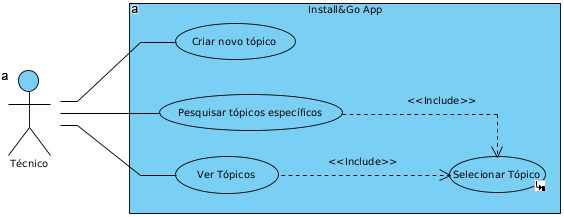
\includegraphics[width=0.6\textwidth]{images/diagramas/casos_de_uso/use_case_forum.png}
    \caption{Diagrama de casos de uso de fórum}
    \label{fig:12}
\end{figure}

\subsubsection{Casos de uso de pesquisar tópicos}

O técnico poderá realizar a pesquisa por tópicos específicos, 
esta será ser realizada por escrito onde indica o assunto a pesquisar e poderá ser filtrada.

O técnico terá também a possibilidade de pesquisar por código QR de produto, uma vez que, o servidor da Motorline esteja desenvolvido para tal.

\begin{figure}[htb]
    \centering
    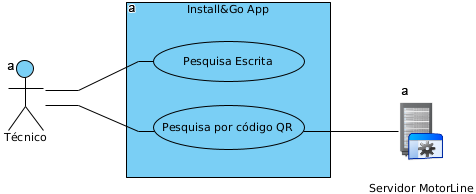
\includegraphics[width=0.6\textwidth]{images/diagramas/casos_de_uso/use_case_forum_search.png}
    \caption{Diagrama de casos de uso de pesquisa de tópicos}
    \label{fig:13}
\end{figure}

\subsubsection{Casos de uso ver detalhes de tópico}

Assim que um técnico seleciona um tópico, é movido para os 
detalhes, onde consegue visualizar os detalhes, responder e, caso seja o seu tópico, consegue finalizar, selecionar a melhor resposta, remover a melhor resposta, eliminar e alterar a visibilidade do tópico.

\begin{figure}[htb]
    \centering
    
    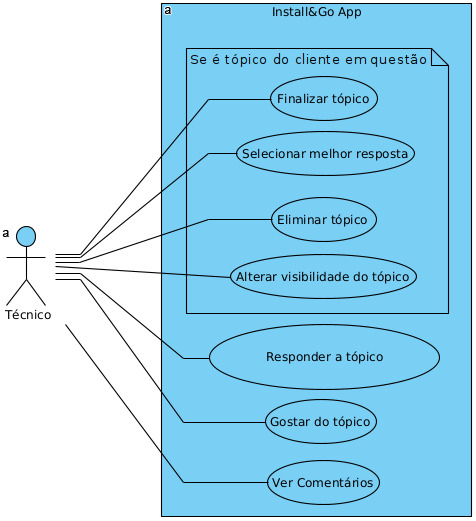
\includegraphics[width=0.5\textwidth]{images/diagramas/casos_de_uso/use_case_topic_details.png}
    \caption{Diagrama de casos de uso de detalhes de tópico}
    \label{fig:14}
\end{figure}

\subsubsection{Casos de uso ver comentários}

O técnico quando decide visualizar os comentários consegue responder e gostar de uma resposta ou comentário, caso este seja seu ainda o consegue apagar.

\begin{figure}[htb]
    \centering
    
    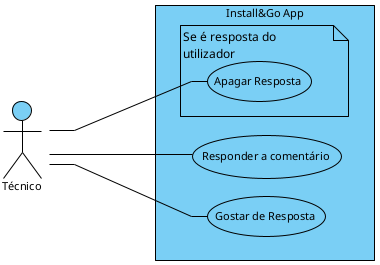
\includegraphics[width=0.5\textwidth]{images/diagramas/casos_de_uso/use_case_topic_comments.png}
    \caption{Diagrama de casos de uso de ver comentários}
    \label{fig:15}
\end{figure}

\subsubsection{Casos de uso ativação de conta}

Assim que uma conta é confirmada, um \textit{email} de ativação é enviado para técnico e esta deverá ser ativada.
Para isto, o código deverá ser indicado pelo técnico para se proceder à ativação da conta. Este, poderá em caso de necessidade, pedir o reenvio do código de ativação, o qual será gerado novamente e reenviado.

\begin{figure}[htb]
    \centering
    
    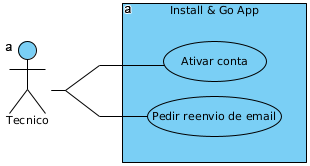
\includegraphics[width=0.5\textwidth]{images/diagramas/casos_de_uso/use_case_account_validation.png}
    \caption{Diagrama de casos de uso de ativação de conta}
    \label{fig:16}
\end{figure}

\subsubsection{Casos de uso perfil}

Sempre que o técnico desejar alterar alguma informação, este poderá alterar o seu nome, \textit{email} e imagem de perfil.

\begin{figure}[htb]
    \centering
    
    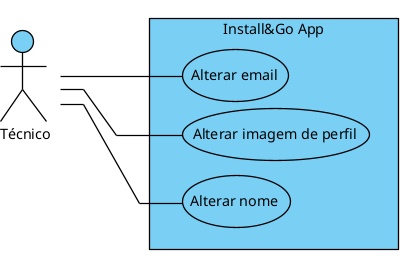
\includegraphics[width=0.5\textwidth]{images/diagramas/casos_de_uso/use_case_perfil.png}
    \caption{Diagrama de casos de uso de perfil}
    \label{fig:17}
\end{figure}

\newpage

\subsubsection{Casos de uso notificações}

Sempre que o técnico desejar ver as suas notificações, poderá seleciona-las, também dispõe da possibilidade de alterar a configuração das notificações, para apenas as receber por \textit{email} ou push, ou então, ambas. Terá também a possibilidade de personalizar cada método, para receber um relatório diário de notificações ou então, notificações em tempo real.

\begin{figure}[htb]
    \centering
    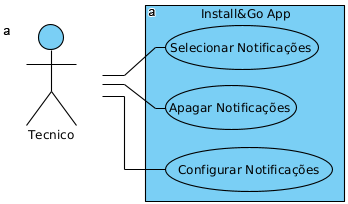
\includegraphics[width=0.5\textwidth]{images/diagramas/casos_de_uso/use_case_notificacoes.png}
    \caption{Diagrama de casos de notificações}
    \label{fig:18}
\end{figure}

\subsubsection{Casos de uso gestão de recursos humanos}

Uma empresa poderá registar contas para os seus técnicos no seu nome, com a indicação do \textit{email} e nºcontribuinte. Esta poderá também impedir acesso a estas contas ou remover completamente a conta da aplicação.

\begin{figure}[htb]
    \centering
    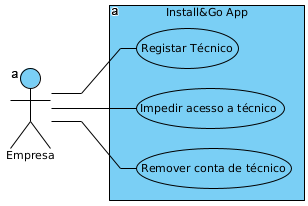
\includegraphics[width=0.5\textwidth]{images/diagramas/casos_de_uso/use_case_rec_humanos.png}
    \caption{Diagrama de casos de uso de recursos humanos}
    \label{fig:19}
\end{figure}

 \newpage
 
 \section{Diagrama Entidade Relação}

O software Install\&Go é suportado por uma base de dados relacional esquematizada de acordo com as necessidades do projeto. Para garantir que os tipos dos atributos se encontram corretos, foram criados novos tipos, já para simular a criação de \textit{id's} do tipo \textit{uuid} foi criado um \textit{stored procedure} o que resulta na tabela de cor verde na Figura\ref{fig:20}. Encontra-se no documento de anexos, no anexo 17, uma versão em maiores dimensões da Figura~\ref*{fig:20}.


\begin{figure}[htb]
  \centering
  
  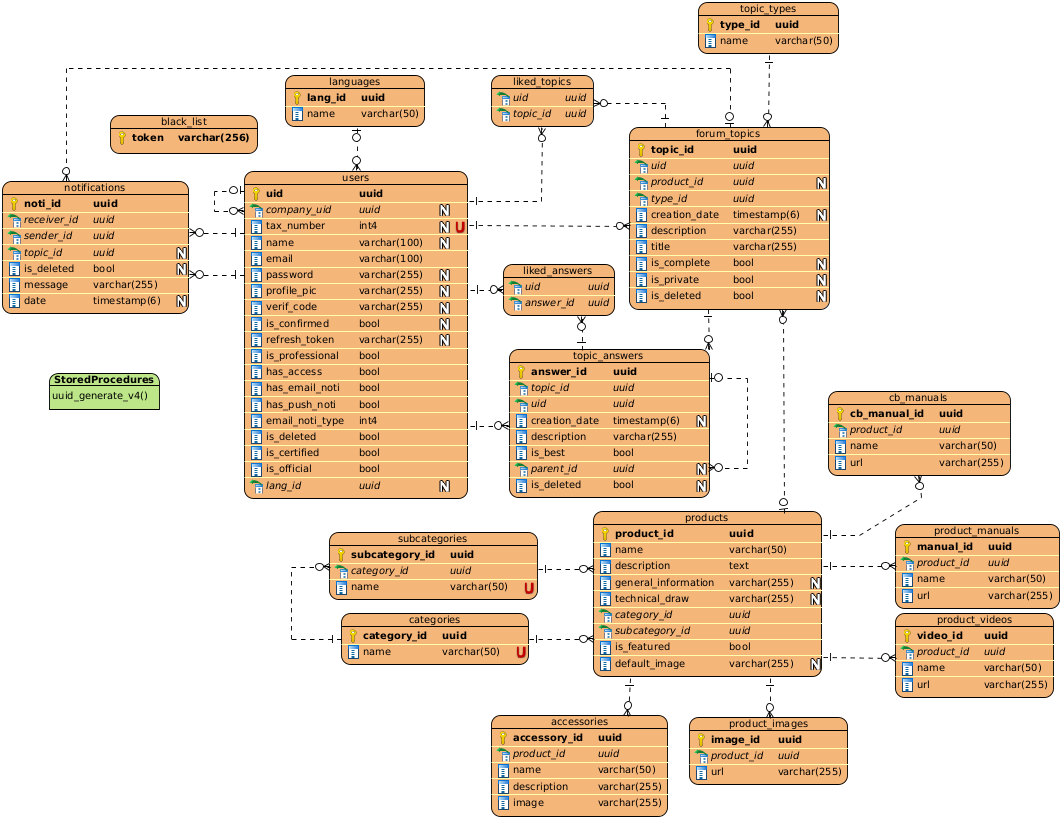
\includegraphics[width=\textwidth]{images/diagramas/diagrama_bd.png}
  \caption{Diagrama Entidade Relação base de dados Install\&Go}
  \label{fig:20}
\end{figure}

\newpage

\subsection{Escolha de diagrama de entidade relação}
Durante o desenvolvimento do diagrama de entidade relação, surgiu 
a opção de separar as empresas dos seus técnicos em duas tabelas como 
exemplificado na Figura~\ref{fig:21}. Neste sempre que se
deseja, por exemplo, obter o utilizador que criou um tópico é necessário
verificar se o \textit{uid} contido é de uma empresa ou de um técnico e apenas de seguida se obter o utilizador que criou o tópico, sendo este um exemplo entre os demais do mesmo tipo. Tendo em conta este problema foi decido optar pelo diagrama da Figura~\ref{fig:20}. Encontra-se no documento de anexos, no anexo 18, uma versão em maiores dimensões da Figura~\ref*{fig:21}.


\begin{figure}[htb]
  \centering
  
  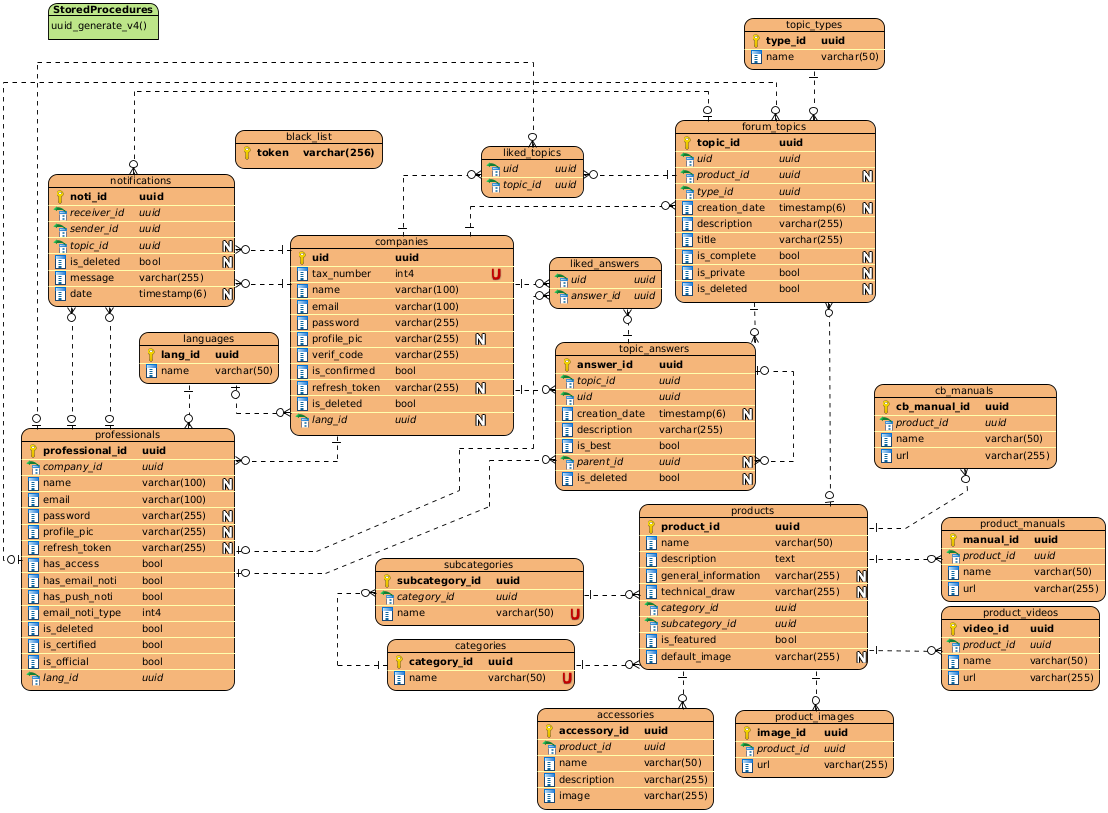
\includegraphics[width=\textwidth]{images/diagramas/diagrama_bd_alt.png}
  \caption{Diagrama Entidade Relação alternativo}
  \label{fig:21}
\end{figure}

\newpage

\subsection{Dicionário de termos}

Com intuito de alcançar o propósito de cada tabela e atributo 
foi criado um dicionário de termos para a base de dados(Tabela~\ref{tab:18}).

\definecolor{Concrete}{rgb}{0.952,0.952,0.952}
\begin{longtblr}
[
caption={Dicionário de termos da base de dados},
label={tab:22},
]{
  width = \linewidth,
  colspec = {Q[220]Q[292]Q[240]Q[215]},
  row{1} = {Concrete},
  column{1} = {c},
  cell{2}{1} = {r=19}{},
  cell{2}{2} = {r=19}{},
  cell{22}{1} = {r=2}{},
  cell{22}{2} = {r=2}{},
  cell{24}{1} = {r=2}{},
  cell{24}{2} = {r=2}{},
  cell{26}{1} = {r=2}{},
  cell{26}{2} = {r=2}{},
  cell{28}{1} = {r=7}{},
  cell{28}{2} = {r=7}{},
  cell{35}{1} = {r=10}{},
  cell{35}{2} = {r=10}{},
  cell{45}{1} = {r=8}{},
  cell{45}{2} = {r=8}{},
  cell{53}{1} = {r=2}{},
  cell{53}{2} = {r=2}{},
  cell{55}{1} = {r=3}{},
  cell{55}{2} = {r=3}{},
  cell{58}{1} = {r=4}{},
  cell{58}{2} = {r=4}{},
  cell{62}{1} = {r=8}{},
  cell{62}{2} = {r=8}{},
  cell{70}{1} = {r=4}{},
  cell{70}{2} = {r=4}{},
  cell{74}{1} = {r=4}{},
  cell{74}{2} = {r=4}{},
  vlines,
  hline{1-2,21-22,24,26,28,35,45,53,55,58,62,70,74,78} = {-}{},
  hline{3-20,23,25,27,29-34,36-44,46-52,54,56-57,59-61,63-69,71-73,75-77} = {3-4}{},
}
Tabela           & Descrição                                                                            & Atributos            & Descrição                                           \\
users            & Tabela encarregue de guardar todos os dados referentes aos utilizadores da aplicação & uid                  & Id do utilizador                                    \\
                 &                                                                                      & company\_id          & Id da empresa referente ao técnico                  \\
                 &                                                                                      & n\_contribuinte      & Número de contribuinte do utilizador                \\
                 &                                                                                      & name                 & Nome do utilizador                                  \\
                 &                                                                                      & email                & Email do utilizador                                 \\
                 &                                                                                      & password             & Password do utilizador                              \\
                 &                                                                                      & profile\_pic         & Imagem de perfil do utilizador                      \\
                 &                                                                                      & verif\_code          & Código de verificação do utilizador                 \\
                 &                                                                                      & is\_confirmed        & Verificação de se o código está confirmado          \\
                 &                                                                                      & refresh\_token       & Token de refresh                                    \\
                 &                                                                                      & is\_professional     & verificação se é profissional                       \\
                 &                                                                                      & has\_access          & verificação se tem acesso à conta                   \\
                 &                                                                                      & has\_email\_noti     & verificação se ativou notificações de email         \\
                 &                                                                                      & has\_push\_noti      & verificação se ativou notificações push             \\
                 &                                                                                      & email\_noti\_type    & tipo de notificação de email                        \\
                 &                                                                                      & push\_noti\_type     & tipo de notificação push                            \\
                 &                                                                                      & is\_deleted          & verificação se a conta se encontra apagada          \\
                 &                                                                                      & is\_certified        & verificação se é um técnico certificado             \\
                 &                                                                                      & is\_official         & verificação se é um técnico oficial                 \\
black\_list      & Tabela que guarda os tokens a bloquear                                               & token                & Token a bloquear                                    \\
liked\_topics    & Tabela encarregue de guardar todos os tópicos que foram gostados pelo utilizador     & uid                  & Id do utilizador                                    \\
                 &                                                                                      & topic\_id            & Id do tópico                                        \\
liked\_answers   & Tabela encarregue de guardar todas as respostas que receberam gosto do utilizador    & uid                  & Id do utilizador                                    \\
                 &                                                                                      & answer\_id           & Id da resposta                                      \\
topic\_types     & Tabela encarregue de guardar os tipos de tópico existentes                           & type\_id             & Id do tipo de tópico                                \\
                 &                                                                                      & name                 & nome do tipo de tópico                              \\
notifications    & Tabela encarregue de guardar todas as notificações do técnico                        & noti\_id             & Id da notificação                                   \\
                 &                                                                                      & receiver\_id         & Recetor da notificação                              \\
                 &                                                                                      & sender\_id           & Emissor da notificação                              \\
                 &                                                                                      & topic\_id            & Id do tópico em caso de estar referente a um tópico \\
                 &                                                                                      & is\_deleted          & verificação se a notificação está apagada           \\
                 &                                                                                      & message              & mensagem da notificação                             \\
                 &                                                                                      & date                 & data de emissão da notificação                      \\
forum\_topics    & Tabela encarregue de guardar todos os tópicos existentes na aplicação                & topic\_id            & Id do tópico                                        \\
                 &                                                                                      & uid                  & Id do dono do tópico                                \\
                 &                                                                                      & product\_id          & Produto referente ao tópico                         \\
                 &                                                                                      & tiype\_id            & Id do tipo referente ao tópico                      \\
                 &                                                                                      & creation\_date       & Data de criação do tópico                           \\
                 &                                                                                      & description          & Descrição do tópico                                 \\
                 &                                                                                      & title                & Titulo do tópico                                    \\
                 &                                                                                      & is\_complete         & Verificação se o tópico está finalizado             \\
                 &                                                                                      & is\_private          & Verificação se o tópico é privado                   \\
                 &                                                                                      & is\_deleted          & Verificação se o tópico está apagado                \\
topic\_answers   & Tabela encarregue de guardar todas as respostas a um tópico                          & answer\_id           & Id da resposta                                      \\
                 &                                                                                      & topic\_id            & Id do tópico                                        \\
                 &                                                                                      & uid                  & Id do dono da resposta                              \\
                 &                                                                                      & creation\_date       & Data de criação da resposta                         \\
                 &                                                                                      & description          & Descrição da resposta                               \\
                 &                                                                                      & is\_best             & Verificação se é a melhor resposta                  \\
                 &                                                                                      & parent\_id           & Id da resposta pai                                  \\
                 &                                                                                      & is\_deleted          & Verificação se o topico se encontra apagado         \\
categories       & Tabela encarregue de guardar todas as categorias de produtos existentes              & category\_id         & Id da categoria                                     \\
                 &                                                                                      & name                 & Nome da categoria                                   \\
subcategories    & Tabela encarregue de guardar as subcategorias de produtos existentes                 & subcategory\_id      & Id da subcategoria                                  \\*
                 &                                                                                      & category\_id         & Id da categoria                                     \\*
                 &                                                                                      & name                 & Nome da subcategoria                                \\*
cb\_manuals      & Tabela encarregue de guardar os manuais de utilização das placas de controlo         & cb\_manual\_id       & Id do manual                                        \\
                 &                                                                                      & product\_id          & Id do produto                                       \\
                 &                                                                                      & name                 & Nome da placa de controlo                           \\
                 &                                                                                      & url                  & Url do manual                                       \\
products         & Tabela encarregue de guardar as informações dos produtos do catálogo da empresa      & product\_id          & Id do produto                                       \\
                 &                                                                                      & name                 & Nome do produto                                     \\
                 &                                                                                      & description          & Descrição do produto                                \\
                 &                                                                                      & general\_information & Url da informação geral do produto                  \\
                 &                                                                                      & technical\_draw      & Url do desenho técnico do produto                   \\
                 &                                                                                      & category\_id         & Id da categoria de produto                          \\
                 &                                                                                      & subcategory\_id      & Id da subcategoria de produto                       \\
                 &                                                                                      & is\_featured         & Verificação se o produto é um destaque              \\
product\_manuals & Tabela encarregue de guardar os manuais de utilização dos produtos                   & cb\_manual\_id       & Id do manual                                        \\
                 &                                                                                      & product\_id          & Id do produto                                       \\
                 &                                                                                      & name                 & Nome do manual                                      \\
                 &                                                                                      & url                  & Url do manual                                       \\
product\_videos  & Tabela encarregue de guardar os videos de cada produto                               & cb\_manual\_id       & Id do video                                         \\
                 &                                                                                      & product\_id          & Id do produto                                       \\
                 &                                                                                      & name                 & Nome dao video                                      \\
                 &                                                                                      & url                  & Url do video                                        
\end{longtblr}

  \newpage

 \section{Diagrama de Classes}

A fim de prever e organizar o \textit{software} foi desenvolvido um diagrama de classes (Figura~\ref{fig:22}) que permite visualizar cada classe que se espera conter no \textit{software}, assim como também os seus atributos e métodos. Encontra-se no documento de anexos, no anexo 13, uma versão em maiores dimensões da Figura~\ref*{fig:22}.

\begin{figure}[htb]
  \centering
  
  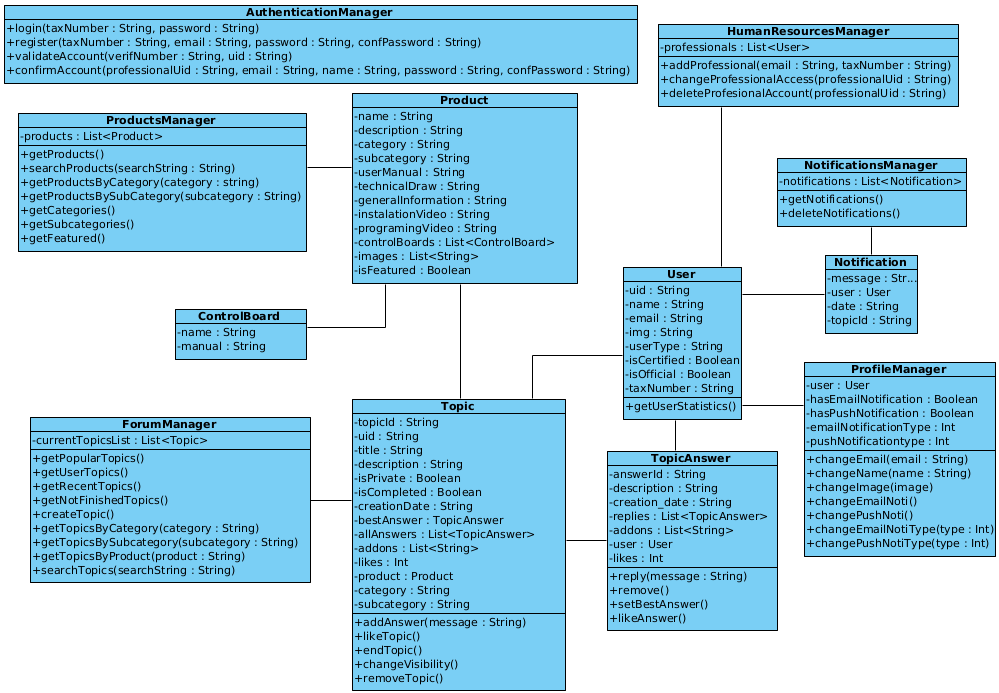
\includegraphics[width=\textwidth]{images/diagramas/diagrama_classes.png}
  \caption{Diagrama de classes Install\&Go}
  \label{fig:22}
\end{figure}


  \newpage

  \section{Mockups}
Com o propósito de criar um \textit{design} para seguir e apresentar às partes interessadas antes de iniciar a fase de desenvolvimento, então foram realizadas \textit{mockups} do \textit{design} da aplicação. Este \textit{design} foi iterativamente revisto pelo cliente e ajustado até alcançar o estado final.

\subsection{Página Inicial}

A página inicial da aplicação, dá ao utilizador a possibilidade de navegar pelos produtos do catálogo, filtrar por categorias e subcategorias, assim como realizar uma pesquisa rápida e por fim navegar para o fórum. Caso um técnico esteja com sessão iniciada este poderá visualizar o \textit{icon} de notificações e a sua imagem de perfil.

\begin{figure}[htb]
    \centering
    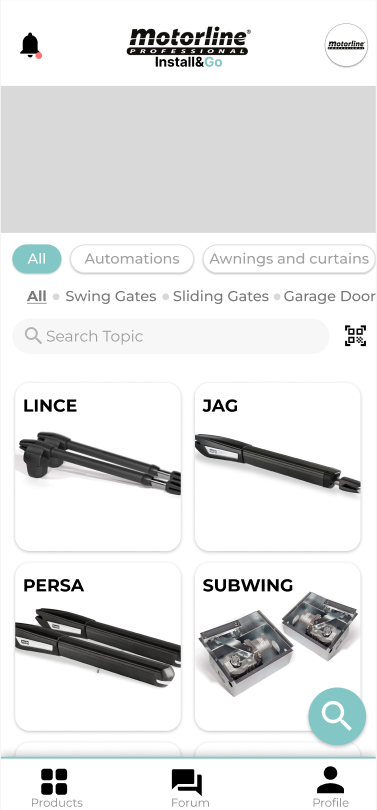
\includegraphics[width=0.45\textwidth]{images/mockups/home_screen.png}
    \caption{Página inicial do fórum}
    \label{fig:23}
\end{figure}

\newpage

\subsection{Autenticação - Login e Registo}

Na autenticação, é possível iniciar sessão e registo, mas a empresa é a única entidade poderá realizar o registo no \textit{software}.

\begin{figure}[htb]%
    \centering
    \subfloat[\centering Página de login]{{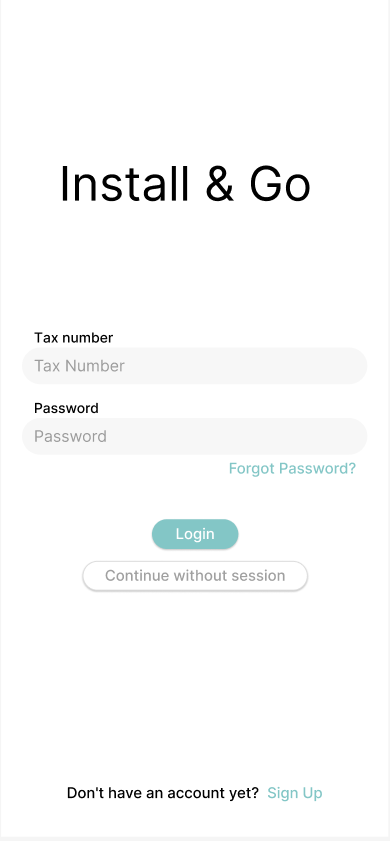
\includegraphics[width=0.4\textwidth]{images/mockups/login.png} }}%
    \qquad
    \subfloat[\centering Página de registo]{{
\includegraphics[width=0.4\textwidth]{images/mockups/register.png} }}%
    \caption{Autenticação - Login e Registo}%
    \label{fig:24}
\end{figure}

\newpage

\subsection{Autenticação - Ativação e Confirmação de conta}

Na autenticação também existe a página de confirmação de conta. Um técnico que tem a conta recentemente adicionada poderá confirmar o registo, indicar as informações finais e por fim será direcionado para a página de ativação onde terá de colocar o código de ativação enviado para o \textit{email}, esta página também será aberta caso um técnico realize o \textit{login} com uma conta que não foi ativada ou sempre que um registo é finalizado.

\begin{figure}[htb]%
    \centering
    \subfloat[\centering Página de confirmação de conta]{{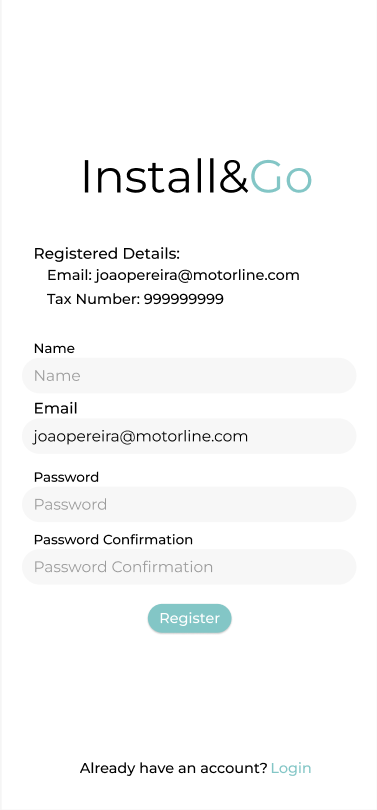
\includegraphics[width=0.4\textwidth]{images/mockups/account_confirmation.png} }}%
    \qquad
    \subfloat[\centering Página de ativação de conta]{{
\includegraphics[width=0.4\textwidth]{images/mockups/account_verification.png} }}%
    \caption{Autenticação - Ativação e Confirmação de conta}%
    \label{fig:25}%
\end{figure}

\newpage

\subsection{Página inicial fórum}

O técnico assim que se dirige ao fórum entrará na página inicial. Esta página permite navegar entre as diferentes listagens de tópicos acessíveis ao técnico, pesquisar, filtrar por tipo e criar um novo tópico.

\begin{figure}[htb]
    \centering
    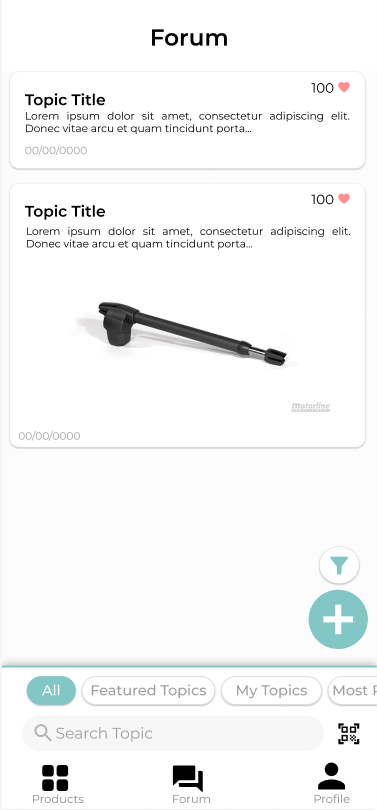
\includegraphics[width=0.45\textwidth]{images/mockups/forum_home.png}
    \caption{Página inicial do fórum}
    \label{fig:26}
\end{figure}

\newpage

\subsection{Página de detalhes de um tópico}

Assim que o técnico seleciona um tópico, será encaminhado para a página de detalhes, onde é indicado o nome do proprietário, a imagem de perfil, a hora de criação, a quantidade de gostos, o título, a descrição, as imagens e os comentários. É possível gostar do tópico, gostar de comentários, comentar o tópico e outros comentários.

Se o tópico for do técnico que está a visualizar, poderá também concluir, eliminar e alterar a sua visibilidade.

\begin{figure}[htb]%
    \centering
    \subfloat[\centering Página de detalhes de um tópico]{{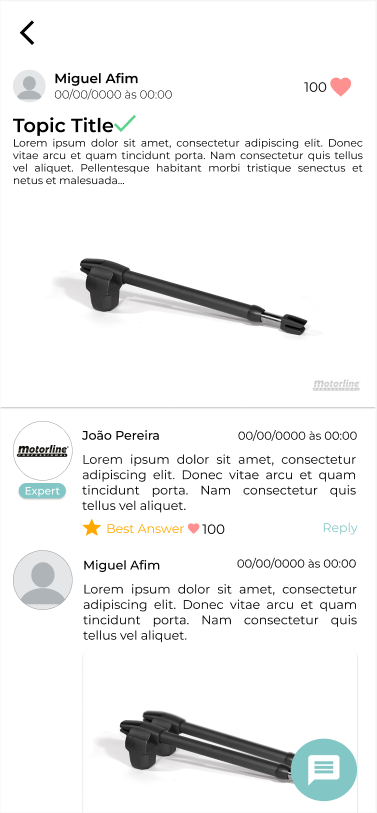
\includegraphics[width=0.4\textwidth]{images/mockups/topic_not_user.png} }}%
    \qquad
    \subfloat[\centering Página de detalhes de um tópico do técnico]{{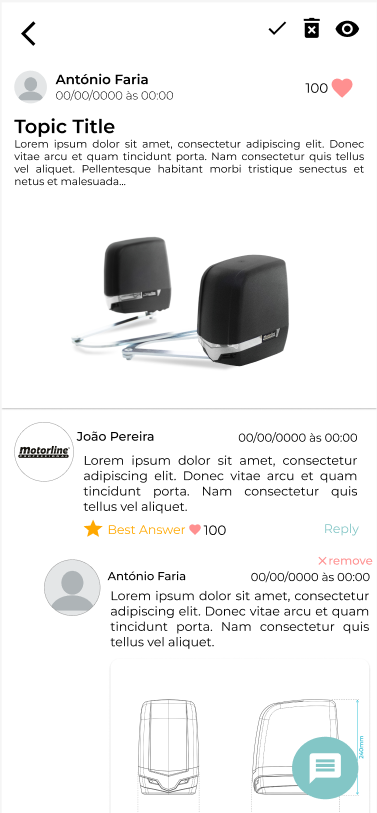
\includegraphics[width=0.4\textwidth]{images/mockups/user_topic.png} }}%
    \caption{Página de detalhes de tópico do software}%
    \label{fig:27}%
\end{figure}

\newpage

\subsection{Página de criação de um tópico}

Quando um técnico inicia a criação de um tópico, é obrigado a inserir o título e a descrição. Já a indicação da visibilidade, do tipo de tópico, do produto referente e de imagens é opcional. A qualquer momento poderá cancelar ou confirmar a ação.

\begin{figure}[htb]
    \centering
    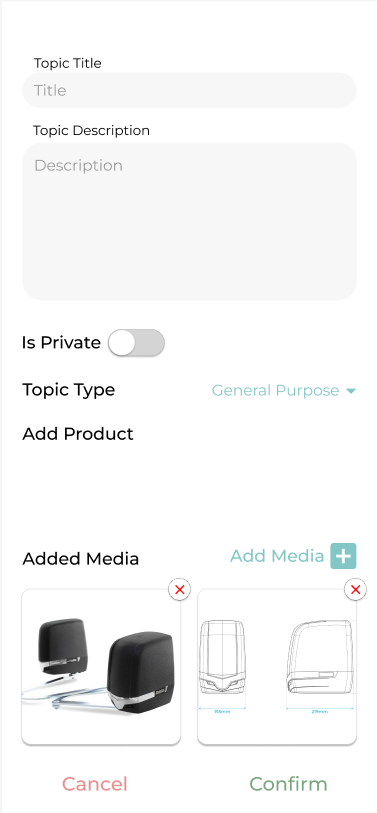
\includegraphics[width=0.45\textwidth]{images/mockups/forum_create_topic.png}
    \caption{Página de criação de tópico}
    \label{fig:28}
\end{figure}

\newpage

\subsection{Página de notificações}

Um técnico sempre que desejar tem como opção visualizar as suas notificações. Neste ecrã, é possível ver todas com a identificação de quem enviou, qual a descrição e a data de receção. O técnico, também tem como escolha apagar se assim desejar.

\begin{figure}[htb]
    \centering
    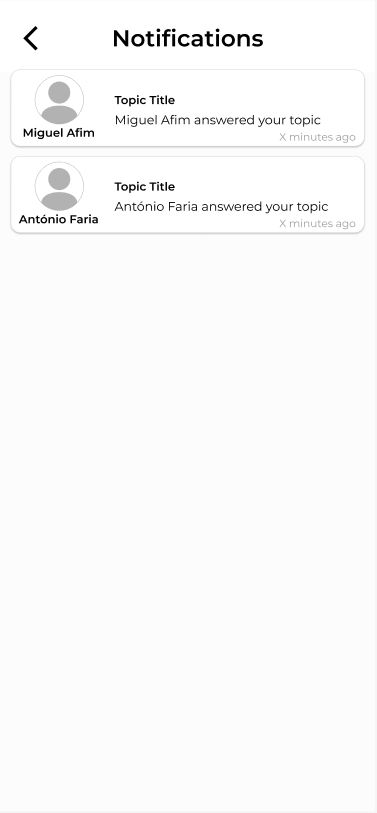
\includegraphics[width=0.45\textwidth]{images/mockups/notifications.png}
    \caption{Página de notificações}
    \label{fig:29}
\end{figure}

\newpage

\subsection{Página de perfil de utilizador}

O técnico, sempre que desejar alterar as suas informações, tem a possibilidade de modificar o \textit{email}, a imagem de perfil e a configuração das notificações com indicação dos métodos e tipo a receber.

Caso uma empresa entre no perfil, esta visualizará um botão para aceder à gestão de recursos humanos.

\begin{figure}[htb]
    \centering
    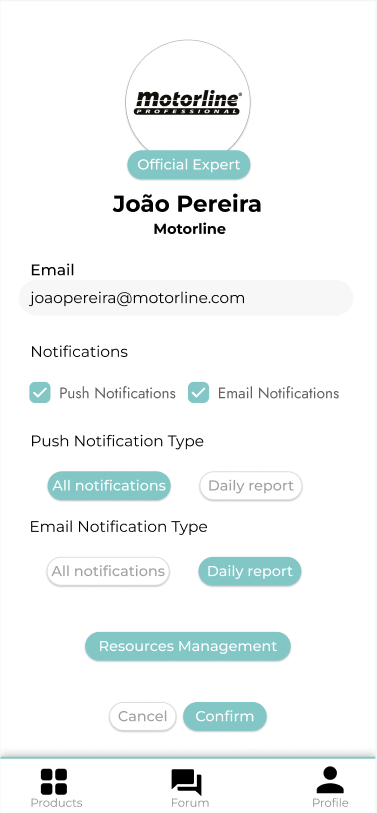
\includegraphics[width=0.45\textwidth]{images/mockups/user_profile.png}
    \caption{Página de perfil de utilizador}
    \label{fig:30}
\end{figure}

\newpage

\subsection{Página de gestão de recursos humanos}

Na página de gestão de recursos humanos, apenas acessível a empresas, é possível registar novos técnicos, pesquisar e gerir os que já se encontram registados através dos seus perfis.

\begin{figure}[htb]
    \centering
    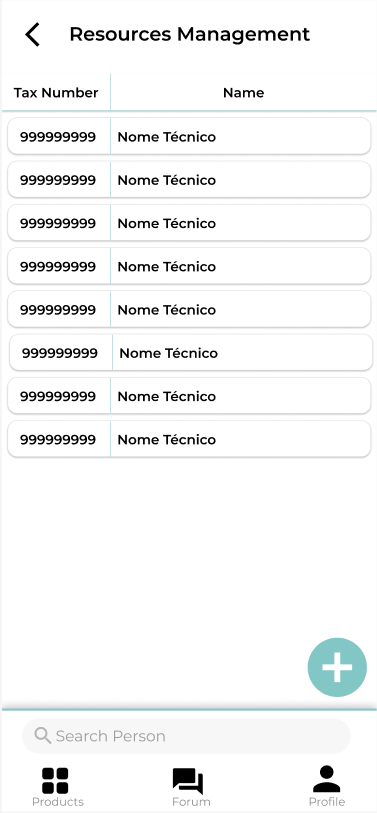
\includegraphics[width=0.45\textwidth]{images/mockups/human_resources.png}
    \caption{Página de gestão de recursos humanos}
    \label{fig:31}
\end{figure}

\newpage

\subsection{Página de perfil de técnico registado}

O perfil de técnico, apenas acessível para empresas, permite visualizar as estatísticas, as informações e permite impedir acesso à conta ou então remover da plataforma.

\begin{figure}[htb]
    \centering
    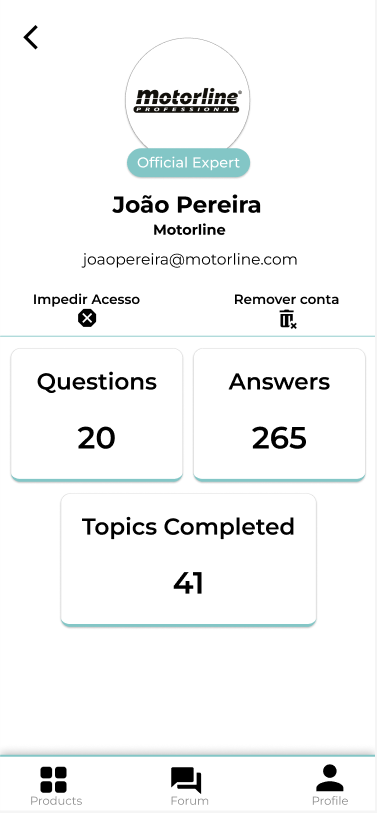
\includegraphics[width=0.45\textwidth]{images/mockups/professional_profile.png}
    \caption{Página de perfil de técnico registado}
    \label{fig:32}
\end{figure}

\newpage

\subsection{Página de registo de novo técnico}

Sempre que uma empresa deseja registar um novo técnico, esta deverá indicar o nome, o \textit{email} e tipo de técnico.

\begin{figure}[htb]
    \centering
    
\includegraphics[width=0.45\textwidth]{images/mockups/account_registering.png}
    \caption{Página de registo de novo técnico}
    \label{fig:33}
\end{figure}

  \newpage

  \section{Diagramas de atividades}
O detalhe de forma simples das ações do ator nos diferentes ecrãs foi realizado em diagramas de atividades.

\subsection{Diagrama de atividades página inicial}

Da página inicial da aplicação é possível deslocar para o fórum, para as notificações, para o perfil e realizar operações do catálogo.

\begin{figure}[htb]
  \centering
  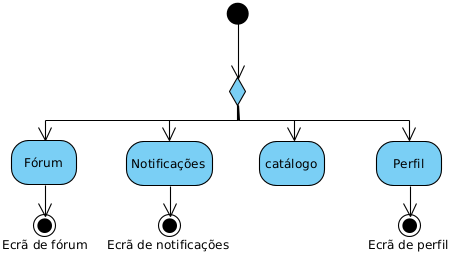
\includegraphics[width=0.6\textwidth]{images/diagramas/atividades/diagrama_atividades_home.png}
  \caption{Diagrama de atividades de página inicial da aplicação}
  \label{fig:34}
\end{figure}

\subsection{Diagrama de atividades página de perfil}

Na página de perfil, é possível alterar a imagem, o nome, o \textit{email}, selecionar os métodos e os tipos de notificação a receber. Caso uma empresa veja o perfil esta poderá, além das operações acima mencionadas, gerir os recursos humanos onde é encaminhada para o ecrã de gestão de recursos humanos.

\begin{figure}[htb]
  \centering
  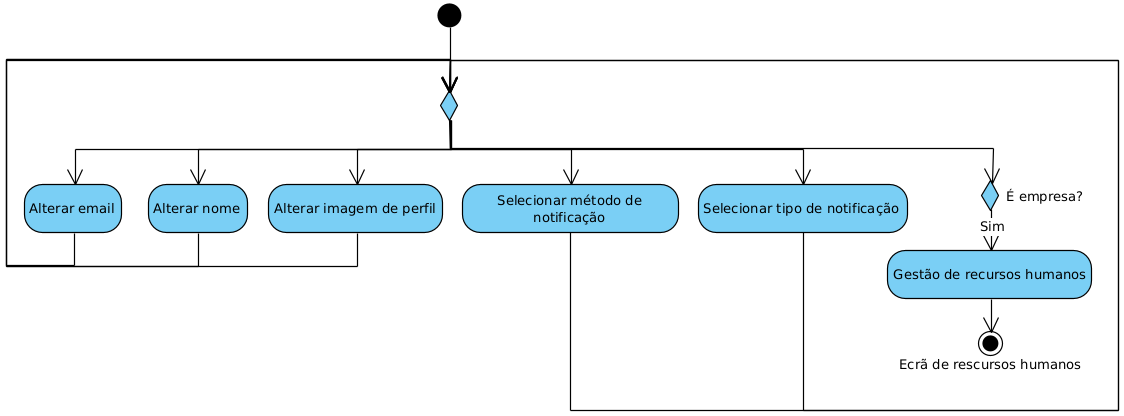
\includegraphics[width=\textwidth]{images/diagramas/atividades/diagrama_atividades_perfil.png}
  \caption{Diagrama de atividades de página de perfil}
  \label{fig:35}
\end{figure}

\newpage

\subsection{Diagrama de atividades página inicial do fórum}

Na página inicial do fórum o técnico poderá selecionar um dos tipos de pesquisa, escrita ou código QR, filtrar por tipo, ver as listagens de tópicos em destaque, mais recentes, por responder, os seus tópicos e criar um novo tópico. Estas listagens poderão ser filtradas por tipo e sobre as mesmas tem a possibilidade de selecionar um tópico o que o redirecionará para o ecrã de detalhes.

\begin{figure}[htb]
  \centering
  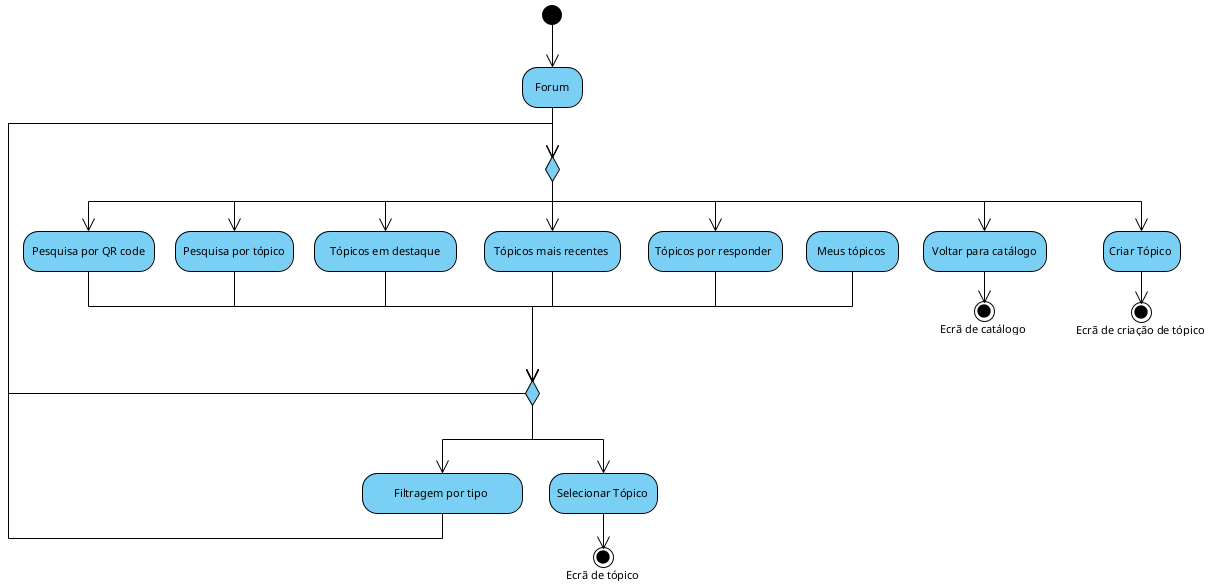
\includegraphics[width=\textwidth]{images/diagramas/atividades/diagrama_atividades_forum.png}
  \caption{Diagrama de atividades de página inicial do fórum}
  \label{fig:36}
\end{figure}

\newpage

\subsection{Diagrama de atividades página de criação de tópico}

Quando o técnico decide criar um tópico, obrigatoriamente tem de indicar o título, a descrição e o tipo do tópico. Por predefinição a visibilidade deste é pública, mas o técnico poderá alterar. Facultativamente o técnico poderá indicar o produto referente ao tópico, assim como anexar e remover imagens. A qualquer momento, o técnico poderá confirmar a criação do tópico, quando esta ação inicia, é realizada uma verificação do título e da descrição para concluir se estão preenchidos. Caso estes dados não estejam preenchidos é indicado ao técnico que as informações estão em falta, caso contrário este volta para o ecrã anterior.

\begin{figure}[htb]
  \centering
  \includegraphics[width=0.7\textwidth]{images/diagramas/atividades/diagrama_atividades_criar_tópico.png}
  \caption{Diagrama de atividades de página de criação de tópico}
  \label{fig:37}
\end{figure}

\newpage

\subsection{Diagrama de atividades página de detalhes do tópico}

Assim que o técnico seleciona um tópico, este poderá visualizar todos os comentários, apagar um caso seja seu, gostar do tópico e/ou de uma resposta, comentar e responder a um comentário. Caso o tópico seja do técnico, este poderá também alterar a visibilidade, marcar como concluído ou remover. A qualquer momento, o técnico tem como possibilidade retroceder para o ecrã anterior.

\begin{figure}[htb]
  \centering
  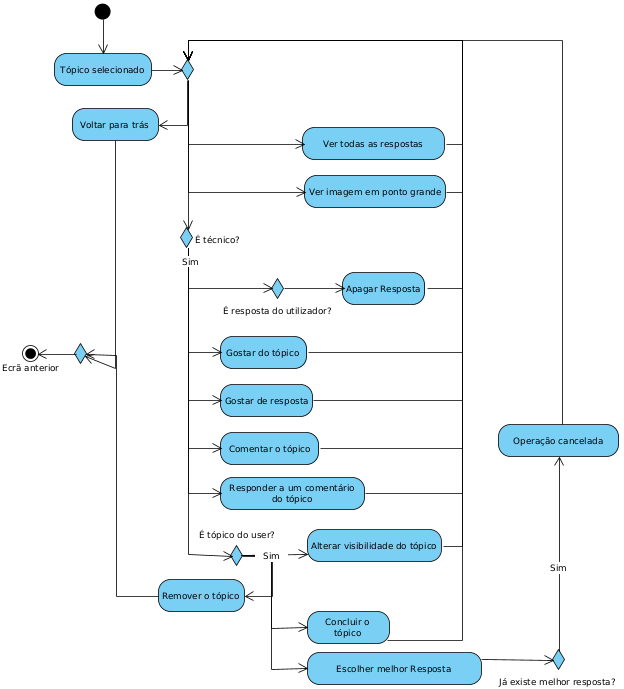
\includegraphics[width=0.9\textwidth]{images/diagramas/atividades/diagrama_atividades_detalhes_topico.png}
  \caption{Diagrama de atividades de página de detalhes do tópico}
  \label{fig:38}
\end{figure}

\newpage

\subsection{Diagrama de atividades páginas de autenticação}

Para realizar a ativação da conta do técnico, assim que este realiza o registo, confirmação da conta ou o login com uma conta que não se encontra ativa, este é encaminhado para o ecrã de ativação da conta. Neste ecrã poderá cancelar e indicar o código de ativação. Se o código estiver errado, o técnico deverá inserir-lo novamente. Por outro lado, se inserir um código correto a conta será validada e o técnico ficará autenticado. Também, em caso de necessidade, o proprietário da conta terá como opção pedir o envio de um novo código de ativação.

\begin{figure}[htb]
  \centering
  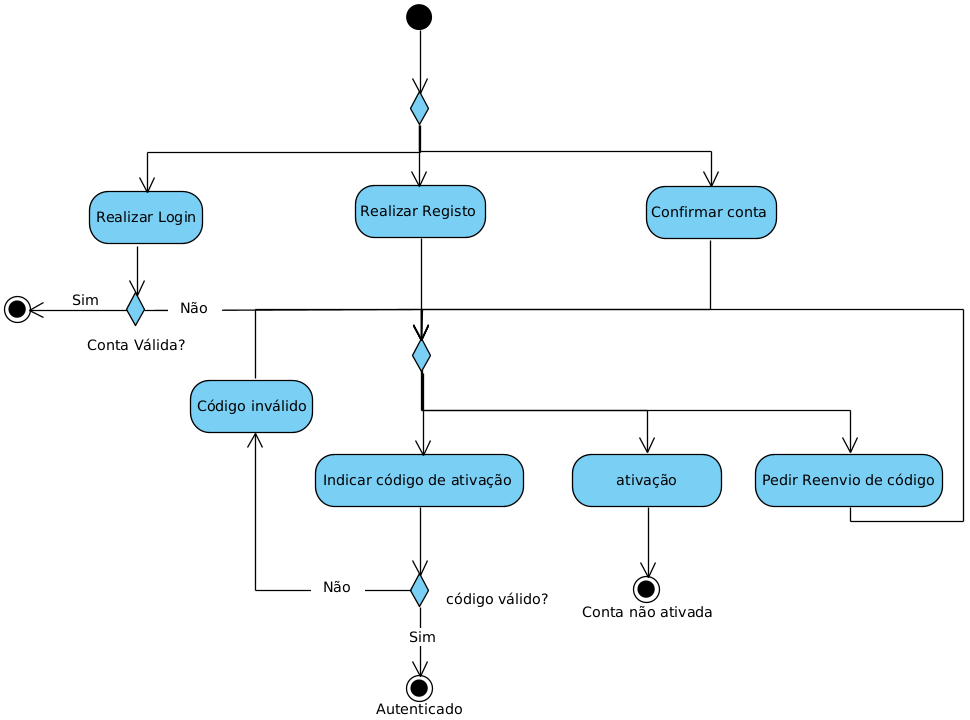
\includegraphics[width=0.8\textwidth]{images/diagramas/atividades/diagrama_atividades_autenticação.png}
  \caption{Diagrama de atividades de página de validação de conta}
  \label{fig:39}
\end{figure}

\newpage

% \subsection{Diagrama de atividades página de notificações}

% Sempre que o técnico recebe uma notificação, este poderá ver esta notificação no ecrã de notificações, 
% Este ecrã permite ao utilizador selecionar uma notificação sendo redirecionado para o tópico referente,
% caso esta esteja referente a um tópico, ou então poderá apagar a notificação.

% \begin{figure}[htb]
%   \centering
%   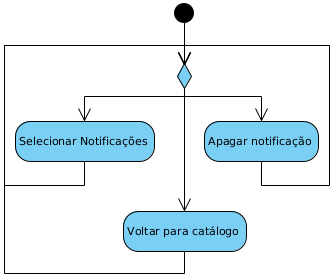
\includegraphics[width=0.5\textwidth]{images/diagramas/atividades/diagrama_atividades_noti.png}
%   \caption{Diagrama de atividades de página de notificações}
%   \label{fig:27}
% \end{figure}

% \subsection{Diagrama de atividades gestão de recursos humanos}

% Uma empresa poderá gerir as contas dos seus recursos humanos, para isso deverá se dirigir a este ecrã.
% Neste ecrã é possível registar um novo técnico sendo encaminhada para o ecrã de registo de técnico, 
% selecionar um técnico sendo encaminhada para o ecrã de perfil do técnico e poderá também pesquisar por 
% técnico.

% \begin{figure}[htb]
%   \centering
%   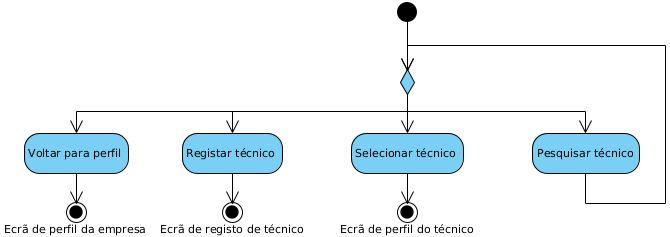
\includegraphics[width=\textwidth]{images/diagramas/atividades/diagrama_atividades_human_resources.png}
%   \caption{Diagrama de atividades de página de recursos humanos}
%   \label{fig:29}
% \end{figure}


% \subsection{Diagrama de atividades perfil de técnico}

% Sempre que uma empresa seleciona um técnico, esta é encaminhada para o ecrã de perfil de técnico. Neste 
% ecrã é possível impedir acesso à plataforma e remover a conta de técnico da plataforma.

% \begin{figure}[htb]
%   \centering
%   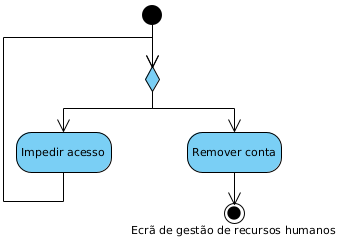
\includegraphics[width=0.5\textwidth]{images/diagramas/atividades/diagrama_atividades_prof_profile.png}
%   \caption{Diagrama de atividades de página de perfil de técnico}
%   \label{fig:30}
% \end{figure}

\newpage

\subsection{Diagrama de atividades registar técnico}

Assim que uma empresa inicia o registo de um técnico, esta é redirecionada para a página de registo do técnico. Nesta página, terá de indicar o nome, o \textit{email} e o tipo de técnico. Por fim será capaz de confirmar o registo da conta e automaticamente a empresa é movida para a página anterior.

\begin{figure}[htb]
  \centering
  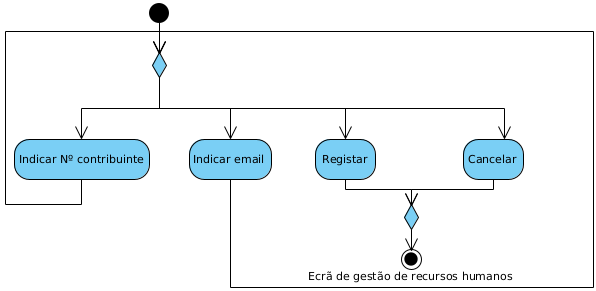
\includegraphics[width=0.8\textwidth]{images/diagramas/atividades/diagrama_atividades_add_professional.png}
  \caption{Diagrama de atividades de página de registar técnico}
  \label{fig:31}
\end{figure}

\subsection{Diagrama de atividades confirmar conta}

Quando uma conta de técnico é registada, um \textit{email} de confirmação é enviado para o técnico. Assim que este o recebe, deverá clicar em confirmar a conta. A partir desta ação, este move-se para a página de confirmação da conta. Nesta página, o técnico poderá alterar o seu \textit{email}, indicar o nome, a \textit{password} e a confirmação da \textit{password}.Todo o processo termina quando o botão de registar for pressionado.

\begin{figure}[htb]
  \centering
  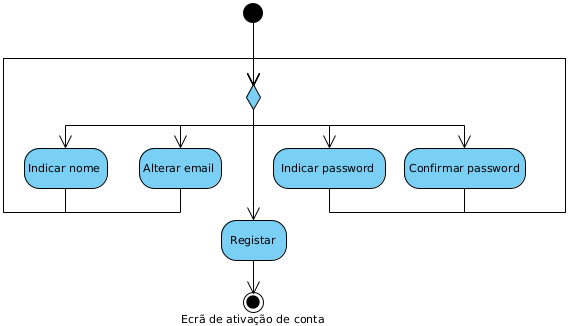
\includegraphics[width=0.8\textwidth]{images/diagramas/atividades/diagrama_atividades_prof_register.png}
  \caption{Diagrama de atividades de página de confirmar conta de técnico}
  \label{fig:31}
\end{figure}

  \section{Diagramas de estados}
Para especificar os principais processos do projeto foram então desenvolvidos diagramas de estados,
sendo então pretendido demonstrar o processo de criação de um tópico do fórum por parte de um técnico, o 
processo de aceder e responder a um tópico e o login com ativação de conta
visto que estas interações são as de maior significância e regradas no software.

\subsection{Diagrama de estados criação de tópico}

Com o diagrama de estados de criação de tópico é pretendido demonstrar o processo de criação de um tópico 
por parte de um técnico. Assim sendo este primeiramente terá de estar autenticado, caso não esteja 
este será encaminhado para autenticação. De seguida criará tópico, após preencher os 
campos desejados este poderá confirmar o tópico, caso confirme é verificado se o tópico possui título, 
caso não possua, é invalido pelo que o técnico deverá preencher os dados em falta, caso o 
título esteja preenchido é verificado se possui descrição e tipo, caso não possua é seguido o mesmo fluxo que o 
caso anterior, caso contrário é criado um tópico. Se o técnico não desejar confirmar o tópico ele 
poderá cancelar, quando assim o faz este torna-se cancelado.

\begin{figure}[htb]
    \centering
    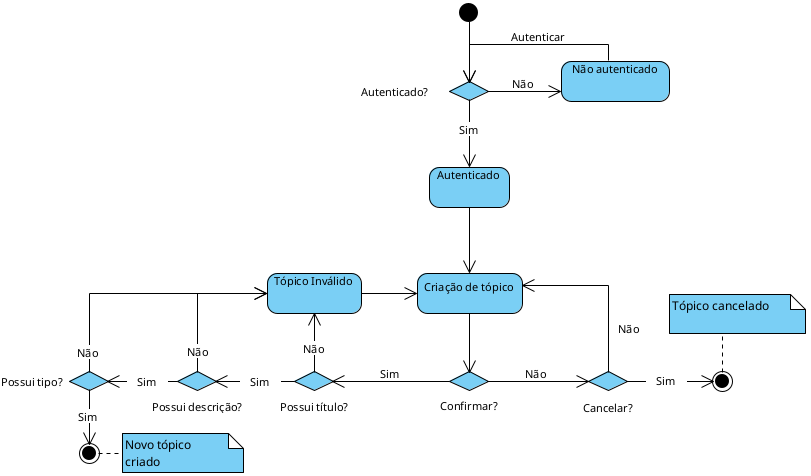
\includegraphics[width=0.9\textwidth]{images/diagramas/estados/criar_topico.png}
    \caption{Diagrama de estados de criar tópico}
    \label{fig:27}
\end{figure}

\newpage

\subsection{Diagrama de estados responder a tópico}

Com o diagrama de estados de responder a tópico é pretendido demonstrar o processo de seleção e 
responder a um tópico por parte de um técnico. Assim sendo que o técnico primeiramente deverá estar 
autenticado, caso não esteja este será encaminhado para a autenticação. Após a autenticação o técnico 
estará autenticado e irá por predefinição ver tópicos em destaque, nesta listagem este selecionará um 
tópico ficando assim o tópico 
selecionado. Assim que o tópico se encontra selecionado o técnico conseguirá responder a este criando 
um comentário. Após a criação do comentário este poderá confirmar o comentário, caso confirme o 
comentário ficará criado, caso contrário este comentário ficará cancelado.

\begin{figure}[htb]
    \centering
    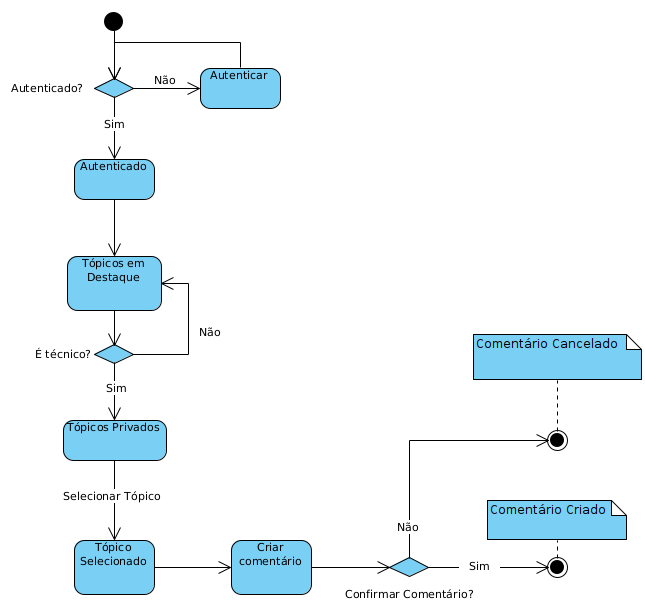
\includegraphics[width=0.7\textwidth]{images/diagramas/estados/responder_topico_tecnico.png}
    \caption{Diagrama de estados de criar tópico}
    \label{fig:28}
\end{figure}

\newpage

\subsection{Diagrama de estados autenticação e validação de conta}

Assim que o técnico decide realizar o login na aplicação este indica as suas credenciais, caso estas 
credenciais não estejam corretas, a autenticação será incorreta e deverá alterar as credenciais. 
Caso as credenciais estejam corretas e a conta válida o técnico ficará autenticado, caso contrário o 
este terá uma conta inválida, pelo que deverá ser validada, para  isso o este deverá 
inserir o código de validação, se o código estiver correto, a conta será validada e o técnico 
ficará autenticado, caso contrário o código será invalido e o deverá indicar o seu código de 
validação novamente.

\begin{figure}[htb]
    \centering
    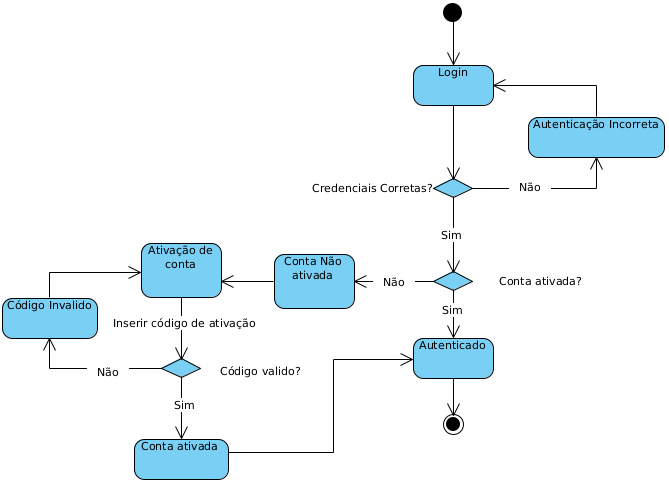
\includegraphics[width=0.7\textwidth]{images/diagramas/estados/autenticacao.png}
    \caption{Diagrama de estados de autenticação e validação de conta}
    \label{fig:29}
\end{figure}


  \newpage

  \newpage

\section{Diagrama de sequência}

Visto que a realização da autenticação, ativação e confirmação de conta requer passos extras e regras a seguir, 
foi necessário criar diagramas de sequência para especificar a sequência de interações do com o sistema.

\subsection{Diagrama de sequência Login e ativação de conta}

Através deste diagrama (Figura~\ref{fig:43}) é entende-se que assim que o técnico deseja realizar o 
login, primeiramente tem de verificar as credenciais, caso estas se encontrem incorretas, este receberá 
uma mensagem de erro, caso as credenciais estejam válidas e a conta esteja ativada o técnico ficará 
autenticado. 

Caso o técnico coloque as credenciais corretas, mas a conta não esteja ativada, este irá realizar a 
ativação de conta, onde poderá enviar o código de ativação, caso esteja correto a sua conta será 
ativada, caso contrário este receberá uma mensagem de erro. Este poderá também cancelar a 
ativação de conta e pedir um novo \textit{email} de ativação, onde será pedido novo código ao servidor, 
este será gerado e enviado.

\begin{figure}[htb]
    \centering
    \includegraphics[width=0.67\textwidth]{images/diagramas/sequencia/diagrama_login.png}
    \caption{Diagrama de sequência de login e ativação de conta}
    \label{fig:43}
\end{figure}

\newpage

\subsection{Diagrama de sequência Registo e ativação de conta}

Através do diagrama abaixo representado (Figura~\ref{fig:44}) é possível perceber que quando uma
empresa realiza o registo este será enviado para o servidor, o qual registará a empresa com uma 
conta não ativada, esta conta será então validada pela Motorline sendo de seguida
gerado um código de ativação e enviado por \textit{email} para o 
\textit{email} de registo, após isto a empresa será encaminhado para a validação de conta, esta validação 
ocorre seguindo o mesmo processo mencionado no anteriormente.


\begin{figure}[htb]
    \centering
    \includegraphics[width=0.8\textwidth]{images/diagramas/sequencia/diagrama_registo.png}
    \caption{Diagrama de sequência de registo e validação de conta}
    \label{fig:44}
\end{figure}

\newpage

\subsection{Diagrama de sequência registo de técnicos}

Através do diagrama abaixo representado (Figura~\ref{fig:45}) é possível perceber que quando uma
empresa deseja registar um técnico, esta introduzirá os seus dados, sendo a sua conta criada. Após isto, 
um código de ativação é gerado e enviado para o técnico ativar a sua conta.

\begin{figure}[htb]
    \centering
    \includegraphics[width=0.8\textwidth]{images/diagramas/sequencia/registo_tecnico.png}
    \caption{Diagrama de sequência de registo de técnicos}
    \label{fig:45}
\end{figure}

  \newpage

 \section{Arquitetura de sistema}
A figura~\ref{fig:46} expõe a arquitetura do sistema que indica as principais componentes. Entre estas, é possível visualizar a aplicação \textit{frontend}, que realiza pedidos a uma aplicação \textit{backend} e espera respostas. O \textit{backend} é composto por uma \textit{api rest} que recebe e responde aos pedidos e por uma base de dados a qual recebe \textit{queries} e devolve dados para a \textit{api rest}. Encontra-se no documento de anexos, no anexo 20, uma versão em maiores dimensões da Figura~\ref*{fig:46}.

\begin{figure}[htb]
  \centering
  
  \includegraphics[width=0.7\textwidth]{images/Arquiteturas/arquitetura_de_solucao.png}
  \caption{Arquitetura do sistema}
  \label{fig:46}
\end{figure}

\subsection{Arquitetura de funcional}
A especificação da implementação da \textit{api rest} foi realizada através de uma arquitetura de \textit{backend}(Figura~\ref{fig:47}). Aqui, é possível visualizar que sempre que a \textit{\acrshort{api}} recebe um pedido, este é redirecionado primeiramente para o \textit{router}. O \textit{router} tem como função identificar a rota referente ao pedido e deslocar para os respetivos \textit{middlewares}. 

Os \textit{middlewares} têm como objetivo realizar todas as ações necessárias antes de proceder à execução do código de rota. Os \textit{middlewares} existentes são o \textit{SessionTokenValidator}, valida a sessão do utilizador a realizar o pedido, de forma similar, o \textit{middleware RefreshTokenValidator}, valida a sessão principal do utilizador e por fim, o \textit{middleware} \textit{RoleValidator}, valida se o utilizador que efetua o pedido tem cargos suficientes para tal. Na eventualidade de não existir nenhum impedimento, o pedido é direcionado para o \textit{controller}.

O \textit{controller} extrai os dados do pedido, verifica se os dados obrigatórios existem e cumprem as regras de negócio e encaminha o pedido para o serviço. O serviço, em caso de necessidade, irá proceder à interação com a base de dados, esta realiza diversas ações como, obter, atualizar, apagar e inserir dados. Por fim, após todo o código de serviço ser executado, a resposta é formulada e devolvida para o utilizador.

Encontra-se no documento de anexos, no anexo 21, uma versão em maiores dimensões da Figura~\ref*{fig:47}.

\begin{figure}[htb]
  \centering
  \includegraphics[width=\textwidth]{images/Arquiteturas/arquitetura_funcional.png}
  \caption{Arquitetura do funcional}
  \label{fig:47}
\end{figure}

\newpage

\subsection{Arquitetura de componentes}
A arquitetura de componentes contém todos os serviços que deverão ser implementados na \textit{api frontend}, com a identificação dos atores que poderão realizar estes pedidos. Esta foi desenvolvida após uma análise de todos os dados necessários para suporte do \textit{frontend}.

\begin{figure}[htb]
  \centering
  \includegraphics[width=0.7\textwidth]{images/Arquiteturas/arquitetura_de_componentes_final.png}
  \caption{Arquitetura de componentes}
  \label{fig:48}
\end{figure}

\newpage

\subsection{Tabela de endpoints}
Com o propósito de evitar colisões de \textit{endpoints} durante a implementação, foi desenvolvida uma tabela de \textit{endpoints}. Esta possui dados semelhantes à arquitetura de componentes (Figura~\ref*{fig:48}), mas para cada serviço é indicada a rota e o método a utilizar.

Encontra-se no documento de anexos, no anexo 25, uma versão em maiores dimensões da Figura~\ref*{docs_swagger}.

% \usepackage{color}
% \usepackage{tabularray}
\definecolor{Concrete}{rgb}{0.952,0.952,0.952}
\begin{longtblr}
[
caption={Tabela de endpoints},
label={tab:19},
]{
  row{1} = {Concrete,c},
  hlines,
  vlines,
}
Serviço                                    & Ator       & Rota                                                             & Método \\
{Obter informações \\do utilizador}        & Cliente    & baseurl/client/:uid                                              & GET    \\
Realizar login                             & Utilizador & baseurl/login                                                    & POST   \\
Realizar registo                           & Utilizador & baseurl/register                                                 & POST   \\
{Esquecimento de \\password}               & Utilizador & baseurl/forgot-password                                          & GET    \\
Ativação de conta                          & Cliente & baseurl/client/:uid/activate                                     & POST   \\
{Reenvio de código \\de ativação de conta} & Cliente & baseurl/client/:uid/new-code                                     & GET    \\
{Obter tópicos em \\destaque}              & Cliente    & baseurl/client/topics/featured                                   & GET    \\
{Obter tópicos mais \\recentes}            & Cliente    & baseurl/client/topics/latest                                     & GET    \\
{Obter tópicos por \\responder}            & Cliente    & baseurl/client/topics/to-answer                                  & GET    \\
{Obter tópicos do \\utilizador}            & Cliente    & baseurl/client/topics                                            & GET    \\
{Obter tópicos \\privados}                 & Técnico    & baseurl/professional/topics/private                              & GET    \\
{Gostar de um \\tópico}                    & Cliente    & baseurl/client/topics/:topicId/like                              & PUT    \\
{Adicionar resposta \\a tópico}            & Cliente    & baseurl/client/topics/:topicId/answer                            & POST   \\
{Adicionar resposta \\a outra resposta}    & Cliente    & baseurl/client/answers/:answerId/                                & POST   \\
{Gostar de uma \\resposta}                  & Cliente    & baseurl/client/answers/:answerId/like                            & PUT    \\
{Marcar tópico \\como completo}            & Cliente    & baseurl/client/topics/:topicId/completed                         & PUT    \\
Remover Tópico                             & Cliente    & baseurl/client/topics/:topicId/                                  & DELETE \\
{Alterar visibilidade \\do tópico}         & Cliente    & baseurl/client/topics/:topicId/visibility                        & PUT    \\
{Adicionar melhor \\resposta do tópico}    & Cliente    & {baseurl/client/topics/:topicId/answers/\\:answerId/best-answer} & PUT    \\
Adicionar novo tópico                      & Cliente    & baseurl/client/topics/                                           & POST   
\end{longtblr}

\begin{figure}[htb]
  \centering
  \includegraphics[width=\textwidth]{images/implementacao/api/swagger_intro.png}
  \caption{Listagem de serviços documentados}
  \label{docs_swagger}
\end{figure}

\newpage

\chapter{Arquitetura de sistema}
Na Figura~\ref{fig:2} é possível visualizar a arquitetura do sistema que indica os principais 
componentes deste software. Entre estes componentes é possível visualizar a aplicação frontend, 
onde esta realiza pedidos a uma aplicação backend e espera respostas. A aplicação backend é composta 
de uma api rest que receberá os pedidos e responderá aos mesmos, este backend é composto também por 
uma base de dados a qual vai receber queries e devolver dados para a aplicação api rest.

\begin{figure}[htb]
    \centering
    
    \includegraphics[width=\textwidth]{images/Arquiteturas/arquitetura_de_solucao.png}
    \caption{Arquitetura do sistema}
    \label{fig:2}
\end{figure}

\newpage

\section{Arquitetura de funcional}

Para especificar a implementação da api rest foi então criada uma arquitetura de 
backend( Figura~\ref{fig:3}), nesta arquitetura é possível visualizar que sempre que a api 
recebe um request este é redirecionado primeiramente para o router, o router tem como função 
identificar a rota a ser pedida e redirecionar para os respetivos middlewares. 

Os middlewares tem como função realizar todo o código necessário antes de proceder à execução 
do código de rota, os middlewares existentes são o SessionTokenValidator, este middleware tem 
como função validar a sessão do utilizador a realizar o pedido, de forma similar o middleware 
RefreshTokenValidator, valida a sessão principal do utilizador, por fim o middleware RoleValidator, 
tem como função validar se o utilizador que realiza o pedido tem cargos suficientes . 
Caso o pedido não seja impedido por nenhum middleware este é então direcionado para o 
controller.

O controller tem como função principal extrair os dados do pedido, validar os dados, verificando 
se os dados obrigatórios existem e encaminhar o pedido para o serviço, procedendo depois à formação 
da resposta e devolução da mesma. No serviço serão primeiramente aplicadas as regras de negócio para 
validar o conteúdo do pedido, caso o pedido não seja impedido por nenhuma das validações de 
regras de negócio, este então, em caso de necessidade, irá proceder à interação com base de dados, 
podendo esta realizar diversas interações como, obter dados, atualizar dados, apagar dados e inserir 
dados. Por fim a resposta é formada e devolvida como resposta ao pedido recebido.

\begin{figure}[htb]
    \centering
    \includegraphics[width=\textwidth]{images/Arquiteturas/arquitetura_funcional.png}
    \caption{Arquitetura do funcional}
    \label{fig:3}
\end{figure}

\newpage

\section{Arquitetura de componentes}
Após a perceção de todas as necessidades da aplicação do frontend, foi então desenvolvida a 
arquitetura de componentes na qual estão contidos todos os serviços que deverão ser implementados na 
api frontend, identificando também qual ator poderá realizar estes pedidos.

\begin{figure}[htb]
    \centering
    \includegraphics[width=0.7\textwidth]{images/Arquiteturas/arquitetura_de_componentes_final.png}
    \caption{Arquitetura de componentes}
    \label{fig:4}
\end{figure}

\section{Tabela de endpoints}
De forma a evitar colisões de endpoints durante a implementação dos mesmos, foi então desenvolvida a 
tabela de endpoints que contém uma estrutura semelhante à arquitetura de componentes, mas que contém 
para cada serviço a rota e o método a utilizar.

% \usepackage{color}
% \usepackage{tabularray}
\definecolor{Concrete}{rgb}{0.952,0.952,0.952}
\begin{longtblr}
[
caption={Tabela de endpoints},
label={tab:19},
]{
  row{1} = {Concrete,c},
  hlines,
  vlines,
}
Serviço                                    & Ator       & Rota                                                             & Método \\
{Obter informações \\do utilizador}        & Cliente    & baseurl/client/:uid                                              & GET    \\
Realizar login                             & Utilizador & baseurl/login                                                    & POST   \\
Realizar registo                           & Utilizador & baseurl/register                                                 & POST   \\
{Esquecimento de \\password}               & Utilizador & baseurl/forgot-password                                          & GET    \\
Ativação de conta                          & Cliente & baseurl/client/:uid/activate                                     & POST   \\
{Reenvio de código \\de ativação de conta} & Cliente & baseurl/client/:uid/new-code                                     & GET    \\
{Obter tópicos em \\destaque}              & Cliente    & baseurl/client/topics/featured                                   & GET    \\
{Obter tópicos mais \\recentes}            & Cliente    & baseurl/client/topics/latest                                     & GET    \\
{Obter tópicos por \\responder}            & Cliente    & baseurl/client/topics/to-answer                                  & GET    \\
{Obter tópicos do \\utilizador}            & Cliente    & baseurl/client/topics                                            & GET    \\
{Obter tópicos \\privados}                 & Técnico    & baseurl/professional/topics/private                              & GET    \\
{Gostar de um \\tópico}                    & Cliente    & baseurl/client/topics/:topicId/like                              & PUT    \\
{Adicionar resposta \\a tópico}            & Cliente    & baseurl/client/topics/:topicId/answer                            & POST   \\
{Adicionar resposta \\a outra resposta}    & Cliente    & baseurl/client/answers/:answerId/                                & POST   \\
{Gostar de uma \\resposta}                  & Cliente    & baseurl/client/answers/:answerId/like                            & PUT    \\
{Marcar tópico \\como completo}            & Cliente    & baseurl/client/topics/:topicId/completed                         & PUT    \\
Remover Tópico                             & Cliente    & baseurl/client/topics/:topicId/                                  & DELETE \\
{Alterar visibilidade \\do tópico}         & Cliente    & baseurl/client/topics/:topicId/visibility                        & PUT    \\
{Adicionar melhor \\resposta do tópico}    & Cliente    & {baseurl/client/topics/:topicId/answers/\\:answerId/best-answer} & PUT    \\
Adicionar novo tópico                      & Cliente    & baseurl/client/topics/                                           & POST   
\end{longtblr}

\newpage

\section{Web scraper}

Após uma reunião com o cliente foi percebido que o catálogo de produtos Motorline não se encontra em um
servidor, esta informação encontra-se apenas diretamente no website da empresa, sendo assim viu-se a 
necessidade de criar um web scraper.

Web scraping é uma terminologia dada para o processo de ler uma página web com o objetivo de obter
informações desta página, geralmente utilizando bots. O grande problema com web scraping é que se não
for realizado com cuidado é possível sobrelotar o servidor da página web.

Sendo assim o scraper irá correr apenas 1 vez por mês visto que o catálogo não é atualizado de forma 
regular. Para agilizar a realização do scraper foi disponibilidado pela empresa a estrutura do website 
a seguir para obter as informações da página web.

\section{falar com prof sobre como integrar isto}
% \chapter{Implementação}



\section{Web scraper}

Após uma reunião com o cliente foi percebido que o catálogo de produtos Motorline não se encontra em um
servidor, esta informação encontra-se apenas diretamente no website da empresa, sendo assim viu-se a 
necessidade de criar um web scraper.

Web scraping é uma terminologia dada para o processo de obter uma página web, ler a página e obter
dados desta, geralmente utilizando bots. O grande problema com web scraping é que pode ser facilmente
detetado. Tendo em conta este problema surgiram duas grandes formas principais de realizar web scraping,
a mais comum sendo realizar um pedido para obter uma página web e ler então esta, sendo assim um processo
rápido e simples. A segunda forma de realizar web scraping é através da simulação da ação humana 
conseguindo abrir o navegador pesquisar pela página desejada, descarregar a página e daí ler esta, 
tornando-se então em um processo lento e complexo.A grande diferença entre estas duas formas é a 
velocidade, visto que a segunda forma tem de esperar que o navegador inicie, de seguida terá de 
esperar que a página carregue e apenas após este processo poderá ser lida a página web.

Na reunião mencionada anteriormente foi decidido que o web scraper iria apenas correr 1 vez por mês
de forma a evitar a sobrelotação do servidor, não existindo problema visto que o catálogo não é 
atualizado regularmente. Para agilizar a realização do web scraper foi disponibilidado pela 
empresa a estrutura do website a seguir para obter as informações da página web.

\newpage

\subsection{Implemenção web scraper}
De forma a implementar e testar o web scraper sem sobrelotar o servidor, foi então descarregado todo
o wesite localmente, conseguindo assim simular o mesmo.

Para implementar o web scraper foi optado pela abordagem mais simples, realizar um pedido para obter a
pagina web, ler a página para obter os dados e guardar os dados.

Para isto foi optado pela linguagem python devido à facilidade desta lidar com grandes quantidades 
de dados. De forma a facilitar a localização dos dados na página foi utilizada a biblioteca bs4, também
conhecida como beautiful soup, esta biblioteca permite alimentar com uma página web e de seguida realizar
pesquisas sobre esta página baseado em tags e atributos dos elementos.

Tendo esta base em conta foi então primeiramente estudado que dados seriam necessários, sendo estes então:
\begin{enumerate}
    \item Categorias e subcategorias de produtos;
    \item Produtos de cada categoria e subcategoria;
    \item Documentação dos produtos;
    \item Imagens e videos dos produtos;
\end{enumerate}

\newpage

Para guardar estes dados foi utilizado um dicionário que contém primeiramente como chaves as categorias de produtos,
para cada categoria contém mais um dicionário com as subcategorias de produtos e para cada categoria existe uma lista
de produtos, contendo o nome de produto, imagem de amostra e url do mesmo.Por fim a chave produtos contém a lista de 
todos os produtos, sendo cada produto representado também por um dicionário, que contém como chaves os atributos do mesmo.
A utilização dicionarios e listas para guardar estes dados deve-se a que o objetivo será guardar estes dados 
em json e a transformação é simplificada utilizando estas estruturas devido à sua proximidade com a estrutura
json.

\begin{figure}[htb]
    \centering
    
    \includegraphics[width=0.7\textwidth]{images/implementacao/scraper/estrutura_scraper.png}
    \caption{Estrutura dos dados obtidos}
    \label{fig:49}
\end{figure}

\newpage

Após uma análise da estrutura do website foi percebido que a página geral de produtos possui todas as categorias
de produtos, assim como também as subcategorias de produtos com urls para as páginas que contém todos os produtos
das subcategorias. Sendo assim foi primeiramente percebido que cada conjunto é uma secção, pelo que é obtido
todas as secções de categorias e para cada uma destas secções é obtido o título da secção que equivale ao nome da
categoria e também todos os correspondentes a clicáveis. Os clicáveis corresponde às subcategorias de cada categoria
estes clicáveis contém também um url que redireciona para a página de produtos da subcategoria.

\begin{figure}[htb]
    \centering
    
    \includegraphics[width=0.55\textwidth]{images/implementacao/scraper/pagina_geral_produtos.png}
    \caption{Página geral de produtos}
    \label{fig:50}
\end{figure}

Sendo assim já é possível identificar cada categoria e subcategoria, assim como também o url da página de produtos
para cada subcategoria. Mas após alguma análise dos dados foi percebido que estas não contem acentuação devido à 
sua formatação no website. Para resolver este problema foi pesquisado por ferramentas capazes de corrigir estes
erros ortográficos. Pelo que foi descoberto que a biblioteca mais utilizada em python para resolver este problema 
é a biblioteca spellchecker, esta ferramenta é a mais utilizada devido à sua capacidade de corrigir erros ortográficos
em diversas linguagens. Sendo assim sempre que uma categoria e subcategoria é obtida, antes de ser guardada, esta é corrigida.

Após isto cada url é aberto e são obtidos os urls de produtos e imagens de amostra dos produtos, para isto foi obtido todos os
elementos clicáveis existentes na secção de produtos de cada página, sendo que cada um correponde a um produto, para obter o nome
do produto correspondente foi utilizado o nome contido no url da página de produto, sendo que todos os produtos seguem a mesma 
estrutura, sendo esta, /produtos/nome-produto. Sendo que em urls não é permitido utilizar acentuação e espaços, então todos os 
nomes foram corrigidos utilizando a mesma ferramenta mencionada anteriormente.

\begin{figure}[htb]
    \centering
    
    \includegraphics[width=0.55\textwidth]{images/implementacao/scraper/pagina_produtos_subcat.png}
    \caption{Página de produtos de uma subcategoria}
    \label{fig:51}
\end{figure}

\newpage
Neste momento após correr o código foi percebido que existiam algumas páginas de produtos em que este não conseguia obter produtos,
pelo que um erro era atirado, para perceber exatamente que páginas de produtos este erro acontecia, sempre que um erro era detetado
este url seria adicionado a uma nova chave do dicionario mencionado anteriormente, esta chave tem o nome misses e contém todos os urls
em que algum erro aconteceu. Foi então neste momento que foi percebido que nem todas as páginas de produtos são iguais e após uma
reunião com o cliente este expôs que existem páginas de produtos e de detalhes de produtos que são muito diferentes das restantes.

\begin{figure}[htb]
    \centering
    
    \includegraphics[width=0.7\textwidth]{images/implementacao/scraper/mconnect.png}
    \caption{Página de produtos de uma subcategoria distinta}
    \label{fig:52}
\end{figure}

De forma ao restante do projeto não ser atrasado foi então decidido primeiramente obter todos os produtos que contêm páginas semelhantes,
sendo assim para cada página de produto foi obtido o titulo que corresponde ao nome do produto, de seguida foi obtida a descrição do produto,
o elemento que contém esta tem como id produto-descrição. As imagens dos produtos são disponibilizadas através de urls na secção da galeria do produto, sendo assim são obtidas todas as imagens desta
galeria e de seguida todos os seus urls.

A documentação dos produtos pode ser disponibilizada através de urls para os manuais,
ou com uma lista dropdown com todos os manuais disponiveis para download, sendo assim são obtidos todos os urls da secção de documentação, 
assim como os seus nomes e todas as opções de documentação do dropdown se este existir.

\begin{figure}[htb]
    \centering
    
    \includegraphics[width=0.7\textwidth]{images/implementacao/scraper/pagina_detalhes_produto.png}
    \caption{Página de detalhes de produto, secção inicial}
    \label{fig:53}
\end{figure}

\newpage

As imagens de desenho técnico e informação geral estão disponibilizadas na secção correspondente
ao nome de cada uma, sendo assim obtidas estas secções e caso estas existam são obtidas as imagens e os seus urls.

\begin{figure}[htb]
    \centering
    
    \includegraphics[width=0.7\textwidth]{images/implementacao/scraper/pagina_detalhes_desenhos.png}
    \caption{Página de detalhes de produto, secção de informações}
    \label{fig:54}
\end{figure}

Os videos de produtos estão disponiveis na secção de videos, sendo que cada secção de videos contém o nome do video e por sua vez o video.
Estes videos são demonstrados utilizando um elemento iframe, este elemento contém um url para o video, mas após tentar visualizar este url,
foi percebido que não é possivel obter o vídeo a partir deste. Sendo assim foi investigada a plataforma vimeo, esta é a plataforma que contém
todos os videos de produtos, pelo que para cada um é gerado um id unico e este poderá ser acedido através do url geral da plataforma seguido 
do id do video. Este id está também colocado no elemento iframe, pelo que este é obtido e acrescentado ao url da plataforma conseguindo assim
guardar todos os videos de produtos.

\begin{figure}[htb]
    \centering
    
    \includegraphics[width=0.7\textwidth]{images/implementacao/scraper/pagina_detalhes_videos.png}
    \caption{Página de detalhes de produto, secção de videos}
    \label{fig:55}
\end{figure}

\newpage

\subsubsection{Implemenção no website}

Após se verificar que eram obtidos pelomenos 80\% dos produtos totais foi então decidido testar no website. Para isto foi utilizada a biblioteca
requests, com a qual é realizado um pedido get a cada url necessário para se obter a página web. Assim que o código foi corrido e a resposta analisada
foi percebido que o website bloqueia este tipo de solução recebendo a resposta demonstrada pela figura~\ref{fig:56}

\begin{figure}[htb]
    \centering
    
    \includegraphics[width=0.7\textwidth]{images/implementacao/scraper/forbiden_response.png}
    \caption{Resposta obtida aquando o pedido ao url da página web}
    \label{fig:56}
\end{figure}

Através da resposta obtida foi então percebido que seria necessário alterar a abordagem visto que a abordagem anterior não seria possível utilizar.
A abordagem opcional a seguir seria simular a ação humana abrindo um navegador e pesquisando pelo url desejado. 

Após uma investigação foi descoberto que existem ferramentas que permitem controlar o dispositivo onde correm impedindo a utilização deste enquanto se 
encontram a correr, assim como ferramentas que apenas recebem o navegador a utilizar e abrem uma nova janela deste navegador para realizar a pesquisa.
Visto que o processo de obter os produtos seria demorado, foi optado pela segunda opção visto que seria possivel continuar com trabalho em paralelo com a
obtenção de dados. Sendo assim a ferramenta mais recomendada para realizar esta operação é a biblioteca selenium, esta biblioteca permite realizar exatamente
o processo referido anteriormente com a possibilidade de escalar com multi threading, permitindo abrir diversas janelas do navegador simultaneamente,
diminuindo drasticamente o tempo de execução para obter os dados, esta funcionalidade não foi explorada devido a limitações de hardware, 
mas seria uma importante implementação futura.

Utilizando a biblioteca selenium foi primeiramente indicado qual o navegador a utilizar, neste caso foi escolhido o chrome devido a este já estar instalado
no dispositivo. Após se indicar qual o navegador a utilizar, é necessário para cada página indicar qual elemento esperar que carregue, pois assim que a pesquisa
é efetuada a página poderá demorar a carregar pelo quem se deverá indicar a espera pelo elemento que se deseja obter. Visto que a página carregada poderá não
conter o elemento a obter foi então implementado um tempo de espera máximo de 5 segundos, assim que este tempo expira a operação é abortada e o url é adicionado
à lista de urls com erros.

\newpage


\subsubsection{Melhoria de implementação}

Após se completar o processo foi então decidido melhorar a implementação resolvendo os erros encontrados em urls especificos. De forma a perceber exatamente quais os urls
que possuem erros foi então direcionado os dados obtidos para um ficheiro json. Sendo assim os urls com erros eram os indicados na figura~\ref{fig:57}.

\begin{figure}[htb]
    \centering
    
    \includegraphics[width=0.7\textwidth]{images/implementacao/scraper/urls_erro_iteracao_1.png}
    \caption{Urls com erro primeira interação}
    \label{fig:57}
\end{figure}

Após uma primeira análise foi possível perceber que grande maioria dos erros provém de urls de acessórios de produtos, isto deve-se ao facto de os acessórios de produtos encontrarem-se
na página de produtos de subcategoria e serem tratados como um url de detalhes de produto, sendo assim sempre que se trata de um url de acessórios seria necessário correr código para 
obter dados de destes ao invés de detalhes de produtos. Para desenvolver este código foi primeiramente analisada a página de acessórios de produtos(Figura~\ref*{fig:58}), 
esta página contém para cada acessório um elemento do tipo artigo o qual contém uma imagem, titulo e descrição, esta descrição por vezes contém urls para os produtos aos quais este acessório se refere, pelo que sempre que estes
urls são detetados, os nomes dos produtos são guardados para futuramente realizar a ligação entre os acessórios e os produtos, visto que não existem produtos com nomes iguais. Foi percebido que nos urls a palavra accessórios está 
sempre contida pelo que sempre que esta é detetada em um url é corrido o código referente à obtenção de acessórios.

\begin{figure}[htb]
    \centering
    
    \includegraphics[width=0.5\textwidth]{images/implementacao/scraper/pagina_acessorios.png}
    \caption{Exemplo de página de acessórios}
    \label{fig:58}
\end{figure}

\newpage

Após correr o novo código criado foi percebido que a quantidade de urls com erros diminuiu, mas existiam produtos com páginas de detalhes de produtos comuns pelo que estas foram analisadas e foi percebido
que um erro ocorria devido a por vezes as páginas não conterem vídeos ou imagens de documentação, sendo que o código foi alterado para apenas obter estes dados se os elementos existirem na página. 
Após correr novamente o código foi percebido que a quantidade de falhas obtidas diminuiu drásticamente (Figura~\ref{fig:59}). Mas mesmo assim ainda existiam 3 falhas a ocorrer e após uma análise foi percebido que
estas falhas estavam a ocorrer devido a:

\begin{enumerate}
    \item Uma página de subcategoria de produtos conter um serviço;
    \item Um produto conter uma página de detalhes de produto com sub produtos;
    \item Existir uma página de adaptadores de produtos;
    \item Um produto conter uma página de detalhes diferente das demais;
\end{enumerate}

\begin{figure}[htb]
    \centering
    
    \includegraphics[width=0.65\textwidth]{images/implementacao/scraper/melhor_corrida.png}
    \caption{Exemplo de página de acessórios}
    \label{fig:59}
\end{figure}



Visto que a página de adaptadores de produtos segue uma estrutura similar à estrutura dos acessórios este foi o primeiro a ser abordado e resolvido, correndo o código de obter detalhes de acessórios sempre a 
palavra acessórios ou adaptadores se encontra no url. De seguida foi percebido que para resolver o problema de existirem serviços e subprodutos o diagrama de base de entidade relação teria de ser alterado pelo que
primeiramente foi resolvido o problema do produto que contém uma página de detalhes diferente das demais. 

Este produto para além da dificuldade de ser uma página completamente diferente as informações encontram-se espalhadas pela página (Figura~\ref*{fig:60}), pelo que estas deveriam ser combinadas para construir os detalhes do produto.
Após a obtenção destes dados foi percebido que as imagens do produto têm dados escritos por cima que não se encontram na imagem original, sendo assim foi
decidido em conversa com o cliente que estas seriam obtidas com screenshots e guardadas num servidor de imagens.

\begin{figure}[htb]
    \centering
    \includegraphics[width=0.7\textwidth]{images/implementacao/scraper/flama.png}
    \caption{Exemplo de página de produto incomum}
    \label{fig:60}
\end{figure}


De forma a resolver o problema de existirem produtos com subprodutos, foi primeiramente alterada a base de dados adicionando uma nova ligação na tabela produtos para ela própria
sendo assim um subproduto possui a chave estrangeira de produto principal preenchida. Após a alteração na base de dados, foi então seguido para a obtenção dos dados do catálogo.
Para os dados foi primeiramente obtido todos os dados do produto principal e de seguida os dados específicos a cada subproduto, sendo que a organização do produto principal é igual
aos restantes mas com um dado extra com os subprodutos. 

\begin{figure}[htb]
    \centering
    \includegraphics[width=0.6\textwidth]{images/implementacao/scraper/zuma.png}
    \caption{Exemplo de página de produto com subprodutos}
    \label{fig:61}
\end{figure}

\newpage

O último problema a solucionar é a existência de serviços, iniciou-se então pela análise do serviço existente, este possui então 
descrição e imagens como os produtos, mas possui também vídeos direcionados a plataformas diferentes, registo de atualizações do serviço
planos de pagamento de serviços, sendo que cada plano contém diversas ofertas e por fim produtos do serviço. 
Possuindo então a estrutura de um serviço foi adicionado à base de dados todas as tabelas de suporte a estes dados e realizadas as ligações necessárias.
Após isto foi percebido que existem dados que não são necessários na descrição pelo que o cliente indicou que seria mais indicado guardar estes dados
como screenshots.
\begin{figure}[htb]
    \centering
    \includegraphics[width=0.6\textwidth]{images/implementacao/scraper/mconnect.png}
    \caption{Exemplo de página de serviço}
    \label{fig:62}
\end{figure}

\subsubsection{Armazenamento de dados}

Após se obter os dados dos produtos, é necessário guardar estes na base de dados para disponibilizar para a sua utilização no backend. Para realizar
esta operação existem duas opções, criar um serviço para inserir produtos e realizar um pedido a este serviço, ou então conectar diretamente
o web scraper à base de dados. Visto que não seria de grande interesse conectar diretamente à base de dados, foi decidido criar um serviço que recebe um produto e o 
insere na base de dados. O grande problema que surgiu com esta solução é que os pedidos ocorrem de forma sequencial, mas com pouco tempo de espera entre estes, o que
levava a que o limite máximo de conexões com a base de dados fosse extrapolado. Isto acontece porque para cada serviço chamado é criado uma nova conexão à base de 
dados, todas as operações são realizadas e por fim a conexão é terminada, mas enquanto estas operações estão a decorrer, o servidor poderá receber mais pedidos, o que 
leva a que mais conexões sejam criadas, atingindo assim rápidamente o limite de conexões da base de dados. Como solução para este problema foi acrescentado uma espera 
de 0.5 segundos a cada pedido. A inserção de serviços decorreu com o mesmo processo.

A inserção de categorias decorre enviando as categorias a inserir em um array, sendo inseridas todas num pedido, já as subcategorias, visto que não se sabe o id da 
categoria referente, foi utilizado o nome da categoria pois este é único, sendo assim é enviado o nome da categoria e as subcategorias referentes, sendo assim todas inseridas
com a referência para a sua categoria.


\newpage

\subsection{Organização do projeto}
Antes de iniciar a implementação, foi definido qual a estrutura de projeto a seguir, pelo que a escolhida foi MVC devido a ser a mais comum e estabelecida. Sendo assim a organização do projeto segue a seguinte estrutura:
\begin{figure}[htb]
  \centering
  \includegraphics[width=0.2\textwidth]{images/implementacao/api/project_organization.png}
  \caption{Exemplo de página de produto incomum}
  \label{fig:63}
\end{figure}

\begin{itemize}
  \item \textbf{docs} - Documentação gerada;
  \item \textbf{src} - Base de todo o projeto;
  \item \textbf{config} - Ficheiros de configuração do projeto;
  \item \textbf{controllers} - Controladores para cada pedido;
  \item \textbf{helpers} - Ficheiros com funções gerais utilizadas regularmente;
  \item \textbf{middlewares} - Ficheiros com os middlewares da api;
  \item \textbf{models} - Classes criadas para representação de base de dados e para as entidades de resposta;
  \item \textbf{routes} - Rotas existentes;
  \item \textbf{services} - Serviços para cada pedido;
  \item \textbf{templates} - Templates de email a serem enviados;
  \item \textbf{tests} - Testes de código realizados;
  \item \textbf{validations} - Validações a realizar a nível de modelo de negócio e validação de dados;
  \item \textbf{app} - Ficheiro de início do projeto;
\end{itemize}

\subsection{Definição de rotas base}
Após a definição da estrutura do projeto foi então definido as rotas base a existir, estas são rotas
que se referem a cada tipo de utilizador. Para melhor organização destas rotas e aplicação de regras foram definidos 3 routers, user para utilizadores se sessão, professional para técnicos e company para empresas. De forma a definir para o projeto qual o router a utilizar em cada pedido foi então definido que:
\begin{itemize}
  \item \textbf{http://baseurl:port/professional} - Encaminhar para router de técnicos;
  \item \textbf{http://baseurl:port/company} - Encaminhar para router de empresas;
  \item \textbf{Restantes} - Encaminhar para router de user;
\end{itemize}

\subsection{Middlewares} 
Um middleware comporta-se como uma ligação entre porções de código, sendo possível este também executar código.

\subsubsection{Linguagem}
O bem essencial em uma boa comunicação entre duas partes é a utilização da mesma linguagem, sendo assim foi necessário perceber qual a linguagem a utilizar quando se responde a um pedido. Para este fim foi então desenvolvido um middleware, o objetivo deste é verificar se existe a chave language no cabeçalho do pedido, caso esta exista é então obtido a linguagem e guardada nas variáveis locais do pedido. Em caso de esta tag não existir, foi então decidido que a aplicação responderá em português por omissão, este valor poderá ser futuramente alterado de forma simples.

\newpage

\subsubsection{Autenticação}
De forma a assegurar a autenticação dos utilizadores que necessitam desta foi então decidido implementar JsonWebToken, este tipo de autenticação baseia-se em a utilização de tokens com tempo de expiração, sendo que enquando o token estiver válido, o utilizador poderá realizar pedidos e assim que este token expirar este terá de se autenticar novamente para obter um novo token.
A utilização de tokens permite também assegurar que os pedidos são realizados com tokens gerados pela api através de utilização de uma chave de assinatura de token, impedindo assim a utilização de tokens gerados por utilizadores.
\begin{figure}[htb]
  \centering
  \includegraphics[width=0.5\textwidth]{images/implementacao/api/jwt_session.png}
  \caption{Exemplo de página de produto incomum}
  \label{fig:64}
\end{figure}

A grande valia da utilização a técnica de autenticação mencionada anteriormente é a segurança desta, mas este nivel de segurança leva a que as aplicações que não necessitam de um nivel de segurança muito alto se tornem impráticas. Isto acontece porque estes  tokens têm geralmente uma duração muito curta como por exemplo 15 minutos, e sempre que um token de sessão expira o utilizador 
teria de realizar novamente o login.

A solução deste problema sem a perda de segurança significativa veio pelo meio da utilização de tokens de duração maior em conjunto com os tokens de duração curta, sendo que enquanto o token de grande duração estiver válido, novos tokens de curta duração são gerados para o utilizador nunca perdendo assim a sua sessão. Estes tokens de grande duração tem por nome tokens de refresh e os tokens de curta duração têm por nome tokens de sessão. Sempre que o utilizador termina a sua sessão o token de refresh deverá ser apagado.

Sempre que um utilizador realiza um pedido o seu token de sessão deverá ser validado, caso este seja válido, o seu token de refresh deverá também ser validado e apenas após isto o utilizador estará autenticado. Caso o token de sessão ou de refresh esteja expirado, este continuará a estar sem autorização para realizar o pedido, mas poderá pedir um novo token de sessão enquanto o seu token de refresh estiver válido, isto acontece sem realizar novamente o login e sem o utilizador perceber.

 Além das funcionalidades atrás mencionadas é possível também associar dados em formato json a um token jwt, esta funcionalidade foi utilizada para enviar o id do utilizador a qual pertence este token e também o cargo do mesmo.

 \newpage

\subsubsection{Validação de Papel}

Com finalidade de garantir que apenas empresas podem realizar os pedidos de empresas e apenas técnicos e empresas podem realizar os pedidos de técnicos foi então criado um middleware que valida se o utilizador que realizou o pedido tem permissões para o mesmo. Este middleware interliga-se com o middleware anterior pois como mencionado o cargo do utilizador em questão é enviado no token, sendo assim é obtido este cargo e realizada uma comparação, com o cargo desejado. Para isto foram criados 2 middlewares diferentes, um valida o cargo de empresas e o outro o cargo de técnicos. Visto que as empresas podem realizar operações de técnicos então no middleware de técnicos é verificado se o token corresponde a um utilizador empresa ou a um utilizador técnico, já no middleware de validação de empresa é verificado se o utilizador tem cargo de empresa.


% //TODO : Adicionar esquema a mostrar como estes middlewares funcionam


\subsection{Controllers}
Assim que um pedido consegue passar por todos os middlewares sem ser impedido, este é então redirecionado para um controller.
Um controller é %Todo: explicar o que é um controller

\subsubsection{Estruturação dos controllers}
De forma a evitar que o código destes controllers varie em termos de estrutura, foi então decidido desenhar uma estrutura de controller e 
aplicar esta perante o demais código. A estrutura deste segue as seguintes etapas:
\begin{enumerate}
 \item Obter dados do pedido
 \item Validar se os dados obrigatórios são obtidos
 \item Validar o pedido perante o modelo de negócio
 \item Executar a lógica do pedido
 \item Formular a resposta e enviar
 \item Em caso de erro este deverá ser capturado e processado de forma a enviar um erro para o utilizador
\end{enumerate}

Para garantir que esta estrutura sempre será aplicada foram utilizados snippets de código que permitem criar um modelo de estrutura de código sendo apenas necessário escrever a palavra chave e toda a estrutura é escrita, necessitando de seguida de efetuar as alterações necessárias perante 
o contexto.

\newpage

\subsubsection{Execução da lógica de negócio}
A execução da lógica de negócio passa por direcionar os dados para a ação correta, sendo que esta ação geralmente resulta em uma operação de base de dados. Inicialmente foi desenvolvida toda a validação de código e todas as operações de base de dados diretamente na execução da lógica de negócio, após uma revisão desta organização de código com o professor orientador, foi decidido separar esta funcionalidades, surgindo assim a componente de validação de dados, a componete de operações de base de dados e por fim a componente de lógica de negócio que implementa a componente de operações de base de dados. Sendo assim de forma a evitar que estas operações sobre a base de dados estejam em conjunto com o direcionamento dos dados, foram então criados modelos para cada tabela. Cada modelo contém um conjunto de operações sobre a sua tabela correspondente, estas operações estão contidas sobre métodos que podem receber dados para executar na operação e devolver a resposta da mesma.

\subsubsection{Validação dos dados}
A validação dos dados é necessária de forma a evitar erros a nivel de servidor com dados em falta e também para aplicar as regras de negócio, garantindo assim que estas são cumpridas. Para realizar estas validações é primeiramente verificado que todos os dados são recebidos, de seguida estes são enviados para um validador. O validador executa todas as verificações necessárias a nivel de regras de negócio e em caso de alguma regra não ser cumprida, é então atirado um erro.

\subsubsection{Formulação da resposta}
Assim como mencionado anteriormente o bem mais importante numa boa comunicação é a utilização da mesma linguagem, sendo assim a resposta do servidor deverá  utilizar a linguagem indicada pelo utilizador. De forma a realizar esta tradução foi utilizado o mesmo conceito que é utilizado para a tradução de aplicações android onde nestas é criado um ficheiro que contém um conjunto de chaves e a cada chave corresponde um texto, para cada tradução estas chaves têm de existir de forma a ser possível obter o texto correto para cada chave. Sendo assim foi utilizado um ficheiro json contento as chaves das linguagens suportadas, a cada linguagem corresponde um conjunto de outras chaves que contém todas as traduções necessárias, utilizando neste caso numeração, em vez de palavras. Esta abordagem permite que de forma fácil futuramente seja possível adicionar outras linguagens ao servidor.

% todo mostrar exemplo

Para dar suporte a este ficheiro foi criada uma operação que recebe a chave desejada e a linguagem desejada, devolvendo o texto correspondente, sendo assim na Formulação da resposta esta operação é executada indicando a chave da resposta a enviar e a linguagem desejada obtendo o texto traduzido, sendo então este devolvido para o utilizador.

\subsubsection{Processamento de erros}
Visto que não é de interesse enviar para o utilizador erros do próprio servidor, foi então decidido controlar estes, para isso foi criado um erro customizado, tendo este por base o erro da própria linguagem. Este erro recebe por parâmetro o código da tradução da mensagem de erro. Esta abordagem permite também evitar que sempre que um erro é lançado o sistema pare. Mesmo com esta abordagem acontece que sempre que um erro é lançado por base de dados, erro de código ou de biblioteca, o erro original é chamado, pelo que foi decidido que sempre que é detetado um erro que não é do tipo do erro customizado, então será devolvido um erro com mensagem de erro de servidor evitando que dados sensíveis e desnecessários para o utilizador sejam devolvidos.

\subsubsection{Envio de emails}
Como mencionado na apresentação da ferramenta tabular, esta não permite a utilização de acentuação na escrita de emails, sendo assim estes erros necessitam de ser resolvidos. Para permitir que os dados dos emails sejam personalizaveis, como por exemplo dados de utilizador e link para clicar, estes emails são colocados dentro de métodos que recebem por parametro os dados personalizaveis, sendo estes então colocados dentro do html do email, este método por fim devolve em string o html do email a enviar.

Para o envio de emails é ncessario um servidor, sendo assim para vias de teste foi utilizado um servidor gratuito de email sendo este hospedado por DIZER QUEM HOSPEDAVA, após a fase de testes foi então alterado para o servidor de email da empresa permitindo assim que este email seja identificado como empresa Motorline.

A configuração do servidor de emails do nodemailer é realizada através de uma chamada ao objeto 
de servidor indicando as configurações do mesmo que estão no ficheiro .env, esta chamada ao servidor por sua vez devolve um objeto que fornece métodos para enviar emails, sendo este então criado e utilizado sempre que se deseja enviar emails no servidor.


De forma a evitar que sempre que se deseja enviar um email seja necessário indicar todos os dados, foi então criado um método que cria e devolve o objeto de servidor sempre que necessário. Sendo assim sempre que se deseja enviar um email é então primeiramente obtido o objeto do servidor, de seguida é invocado o método para obter o conteúdo html do email e por fim é utilizado o objeto do servidor para chamar o método de envio de emails no qual se terá de indicar o email do destinatário, o assunto e o conteúdo do email.


\newpage

\subsubsection{Logging de erros}

A identificação dos erros no servidor é difícil, pois uma vez que os erros são tratados, os dados referentes aos mesmos não são guardados ou utilizados, para resolver este problema foi então decidido que sempre que um erro que não é customizado é detetado, é registado um log, este contém informações sobre o pedido como data e hora, dados recebidos e assim como também a descrição original do erro e serviço referente.

Para implementar esta solução foi então primeiramente criado um middleware que sempre que deteta erros dentro do serviço executa um método. Este método por sua vez obtém os dados referentes ao pedido realizado, sendo estes a data e hora, os dados recebidos e o serviço pedido. Após se obter os dados do pedido é obtida a mensagem do erro, sendo então estes dados acrescentados em uma nova linha no ficheiro de erros do servidor.

\subsubsection{Logging de pedidos com morgan}

Para realizar o logging de pedidos a serviços foi então utilizado o morgan, esta ferramenta apenas precisa que seja indicado o ficheiro onde escrever os logs, sendo utilizado um ficheiro chamado log, este também precisa de saber qual o tipo de log a realizar, sendo estes tipos indicados pela ferramenta, o tipo utilizado foi o combinado, este é o tipo de log mais completo da ferramenta, visto que é o que obtém mais dados, sendo estes, a data e hora do pedido, o tipo de pedido, o serviço pedido, os dados recebidos, a resposta devolvida e também a descrição do sistema utilizado.

\subsubsection{Agendamento de tarefas}

Utilizando a ferramenta node-cron foi inicialmente programado para este enviar o relatório de notificações todos os dias às 22 horas, para realizar esta configuração e necessário indicar primeiramente a programação de horário de envio, para isso é utilizada a estrutura segundo, minuto, hora, dia do mês, mês, dia da semana. Visto que o objetivo é as 22 horas os segundos e minutos foram indicados como 0 e as horas foram indicadas como 22, já o restante foi indicado com o símbolo "*" que indica que o processo deverá occorrer em todas as instâncias dos restantes valores, significando assim todos os dias. A configuração final obtida foi então "0 0 22 * * *".

Quando o método do agendamento é invocado, é então obtido todos os utilizadores com a configuração de relatório de notificações ativa, sendo de seguida para cada um destes obtidas todas as notificações do dia. De seguida é criado o objeto de servidor e invocado o método para obter o email de notificações enviando todas as notificações do utilizador para o mesmo. Por fim é enviado o email para o utilizador com todas as suas notificações e um link para aceder rápidamente ao ecrã de notificações.

\newpage

\input{sections/chap5/2.servicos_backend/9.segurança.tex}

\subsubsection{Documentação Typedoc}
Durante a implementação desta ferramenta foi detetado que a categorização de documentação não se encontrava funcional devido a um problema encontrado pelos desenvolvedores da ferramenta, foi decidido então reduzir a versão da mesma para uma com a funcionalidade ativada, mas esta não se encontrava compatível com a versão mais atualizada de typescript, pelo que não foi possível explorar esta funcionalidade. Para contornar o problema foi então decidido explorar outra funcionalidade menos utilizada da ferramenta, esta funcionalidade permite converter qualquer documentação em módulos, estes módulos podem então ser categorizados, o problema destes módulos é que cria um modelo genérico do código não sendo fácilmente identificado as tipagens de scripts. Estes módulos permitem também a categorização dos mesmos permitindo assim um nível de organização da documentação gerada.

\newpage

\subsubsection{Documentação Swagger}
Apesar da ferramenta disponibilizar a geração automática de documentação a partir de comentários de código, foram encontrados alguns problemas com esta funcionalidade, acabando por não gerar a documentação, pelo que foi optado por manter a documentação manualmente com o ficheiro json. Esta ferramenta oferece diversas funcionalidades como autenticação, definição de estruturas de dados para os serviços e exemplos de respostas para os mesmos, ambas estas funcionalidades foram exploradas conseguindo assim um bom suporte de documentação para qualquer utilizador.

\begin{figure}[htb]
  \centering
  \includegraphics[width=0.6\textwidth]{images/implementacao/api/swagger_intro.png}
  \caption{Documentação swagger}
  \label{fig:66}
\end{figure}

\begin{figure}[htb]
  \centering
  \includegraphics[width=0.6\textwidth]{images/implementacao/api/swagger_pedido.png}
  \caption{Exemplo de documentação de serviço}
  \label{fig:67}
\end{figure}

\newpage
\section{Frontend}
Um dos requisitos do projeto é o desenvolvimento do frontend utilizando a ferramenta Flutter, visto que a empresa já utiliza esta ferramenta, sendo assim necessário o aprendizado desta ferramenta e da sua linguagem de programação o dart.

\subsection{Flutter}
EXPLICAR O QUE E FLUTTER

\subsection{Dart}
EXPLICAR O QUE É DART

\subsection{Processo de aprendizagem}
De forma a realizar a aprendizagem da ferramenta foi então procedido para a desenvolvedora da mesma, a google, esta dispõe de uma lista de workshops e projetos a seguir de forma a aprender as bases da ferramenta, sendo a lista a seguinte:

\begin{enumerate}
  \item MDC-101 no Flutter: noções básicas dos componentes do Material Design | Google Codelabs
  \item MDC-102 no Flutter: estrutura e layout do Material Design | Google Codelabs
  \item MDC-103 Flutter: temas do Material Design com cores, formas, elevação e tipo | Google Codelabs
  \item MDC-104 Flutter: componentes avançados do Material Design | Google Codelabs
  \item Apps adaptáveis no Flutter | Google Codelabs
\end{enumerate}

Após a realização destes workshops, foi possível entender como funciona a base desta ferramenta e também encontrar fontes para pesquisa de widgets da comunidade a nível gráfico e funcional, provando estes serem de grande auxílio no desenvolvimento da aplicação frontend.
% \chapter{Conclusão e futuras implementações}


\bibliography{biblio}

\end{document}  
